\documentclass[12pt]{extarticle}
\usepackage[paperwidth=18in,paperheight=8.5in]{geometry}
\usepackage{amsmath}
\usepackage{hyperref}
\usepackage{multirow}
\usepackage{pdfpages}
\usepackage[utf8]{inputenc}
\title{Kaon mixing: chiral and continuum extrapolations}
\author{R Mukherjee}
\date{\today}
\begin{document}
\maketitle
\tableofcontents
\clearpage
\begin{figure}
\centering
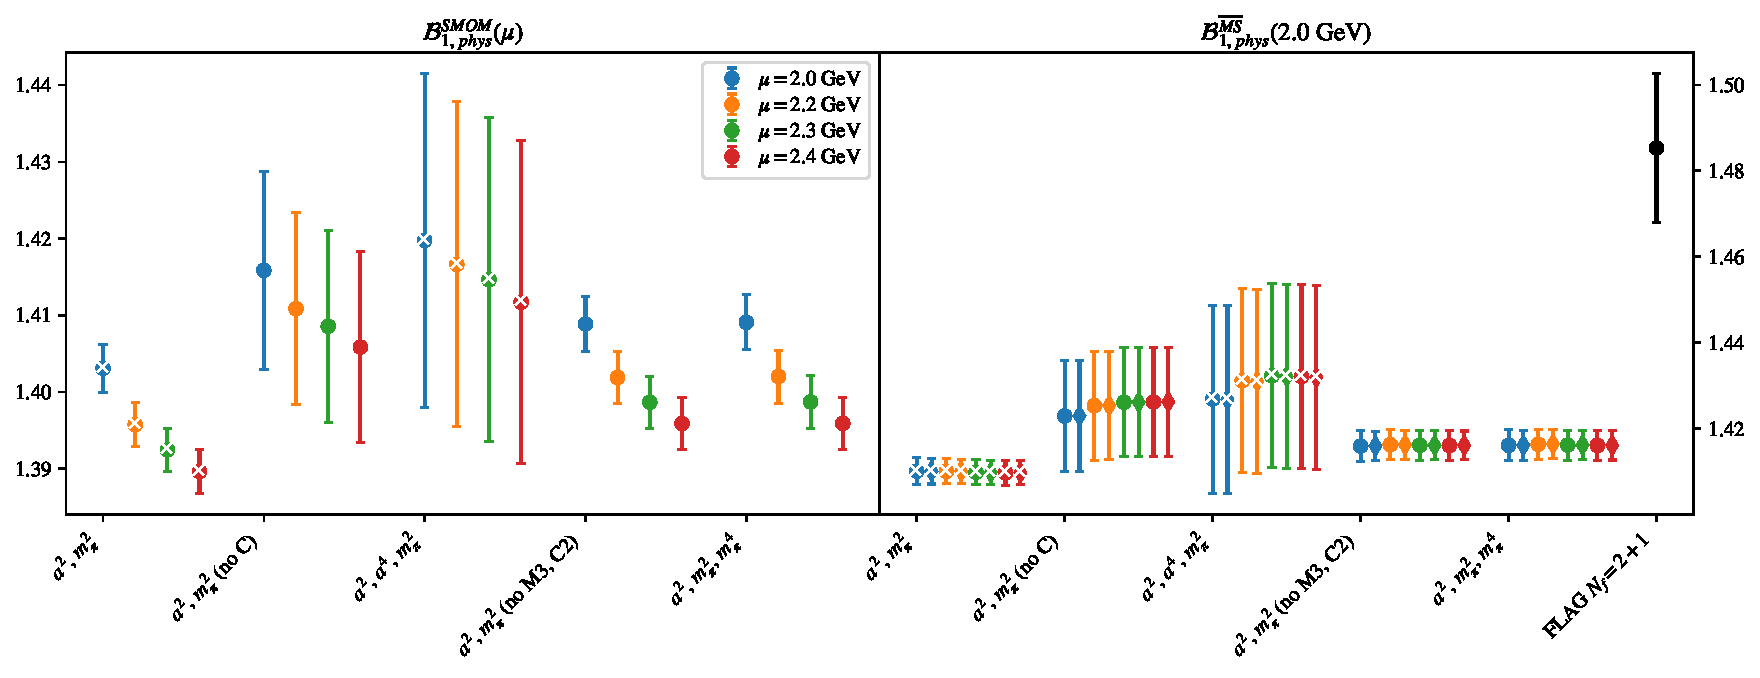
\includegraphics[page=1, width=1.1\textwidth]{VVpAA/SUSY/fit_summary_bag.pdf}
\caption{$\mathcal{B}_{1}$\\(left) $\mathcal{B}_{phys}$ in RI/SMOM scheme from fit variations (fits with $p$-value $<0.05$ marked with ``$\times$"). \\(right) $\mathcal{B}_{phys}$ in $\overline{MS}$ computed using $\mathcal{B}^{\overline{MS}} = R^{\overline{MS}\leftarrow SMOM}(2.0)\sigma_{npt}(2.0,\mu) \mathcal{B}^{SMOM}(\mu)$.}
\end{figure}
\clearpage
\begin{figure}
\centering
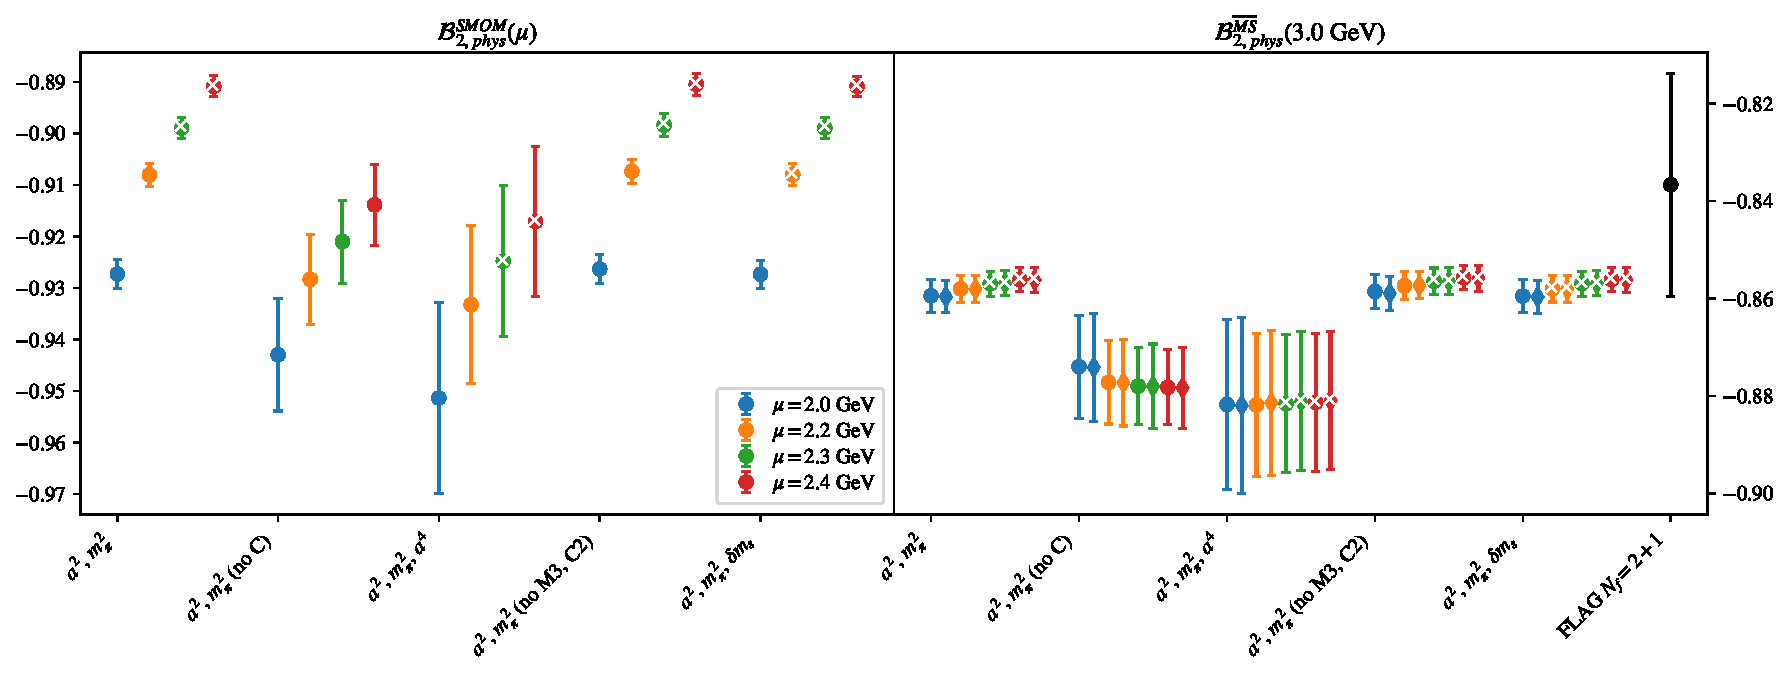
\includegraphics[page=1, width=1.1\textwidth]{VVmAA/SUSY/fit_summary_bag.pdf}
\caption{$\mathcal{B}_{2}$\\(left) $\mathcal{B}_{phys}$ in RI/SMOM scheme from fit variations (fits with $p$-value $<0.05$ marked with ``$\times$"). \\(right) $\mathcal{B}_{phys}$ in $\overline{MS}$ computed using $\mathcal{B}^{\overline{MS}} = R^{\overline{MS}\leftarrow SMOM}(3.0)\sigma_{npt}(3.0,\mu) \mathcal{B}^{SMOM}(\mu)$.}
\end{figure}
\clearpage
\begin{figure}
\centering
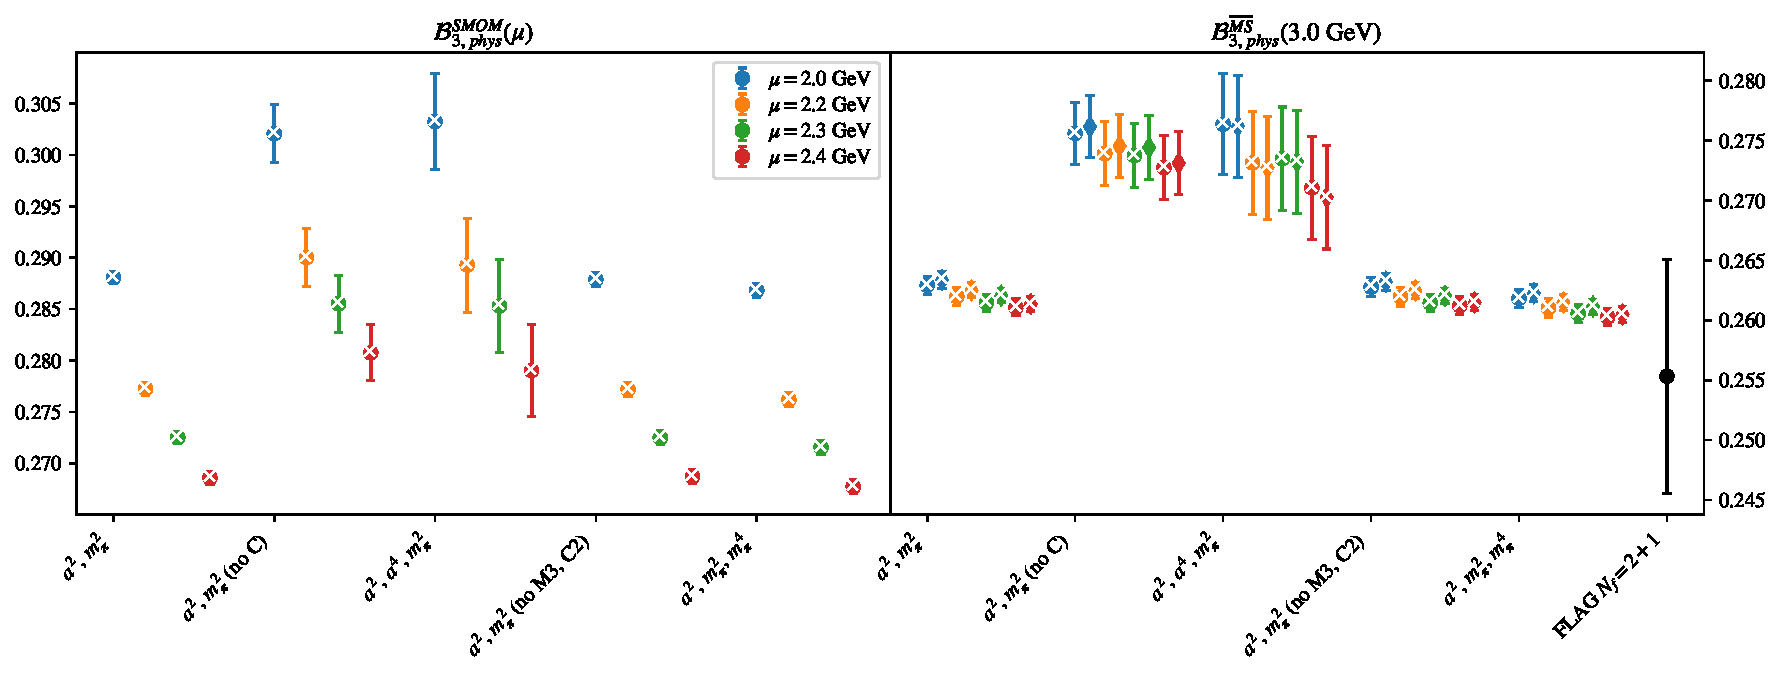
\includegraphics[page=1, width=1.1\textwidth]{SSmPP/SUSY/fit_summary_bag.pdf}
\caption{$\mathcal{B}_{3}$\\(left) $\mathcal{B}_{phys}$ in RI/SMOM scheme from fit variations (fits with $p$-value $<0.05$ marked with ``$\times$"). \\(right) $\mathcal{B}_{phys}$ in $\overline{MS}$ computed using $\mathcal{B}^{\overline{MS}} = R^{\overline{MS}\leftarrow SMOM}(3.0)\sigma_{npt}(3.0,\mu) \mathcal{B}^{SMOM}(\mu)$.}
\end{figure}
\clearpage
\begin{figure}
\centering
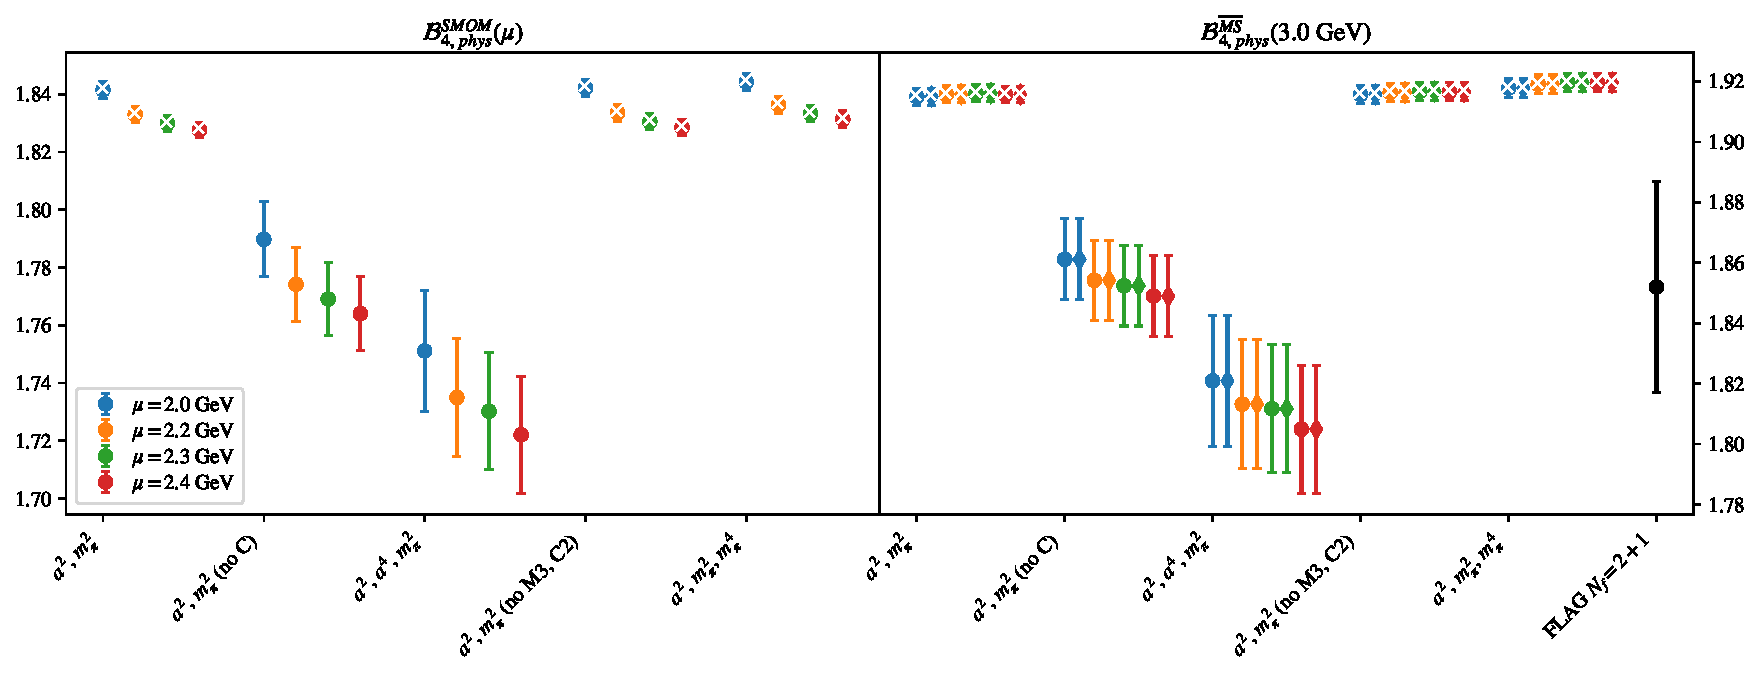
\includegraphics[page=1, width=1.1\textwidth]{SSpPP/SUSY/fit_summary_bag.pdf}
\caption{$\mathcal{B}_{4}$\\(left) $\mathcal{B}_{phys}$ in RI/SMOM scheme from fit variations (fits with $p$-value $<0.05$ marked with ``$\times$"). \\(right) $\mathcal{B}_{phys}$ in $\overline{MS}$ computed using $\mathcal{B}^{\overline{MS}} = R^{\overline{MS}\leftarrow SMOM}(3.0)\sigma_{npt}(3.0,\mu) \mathcal{B}^{SMOM}(\mu)$.}
\end{figure}
\clearpage
\begin{figure}
\centering
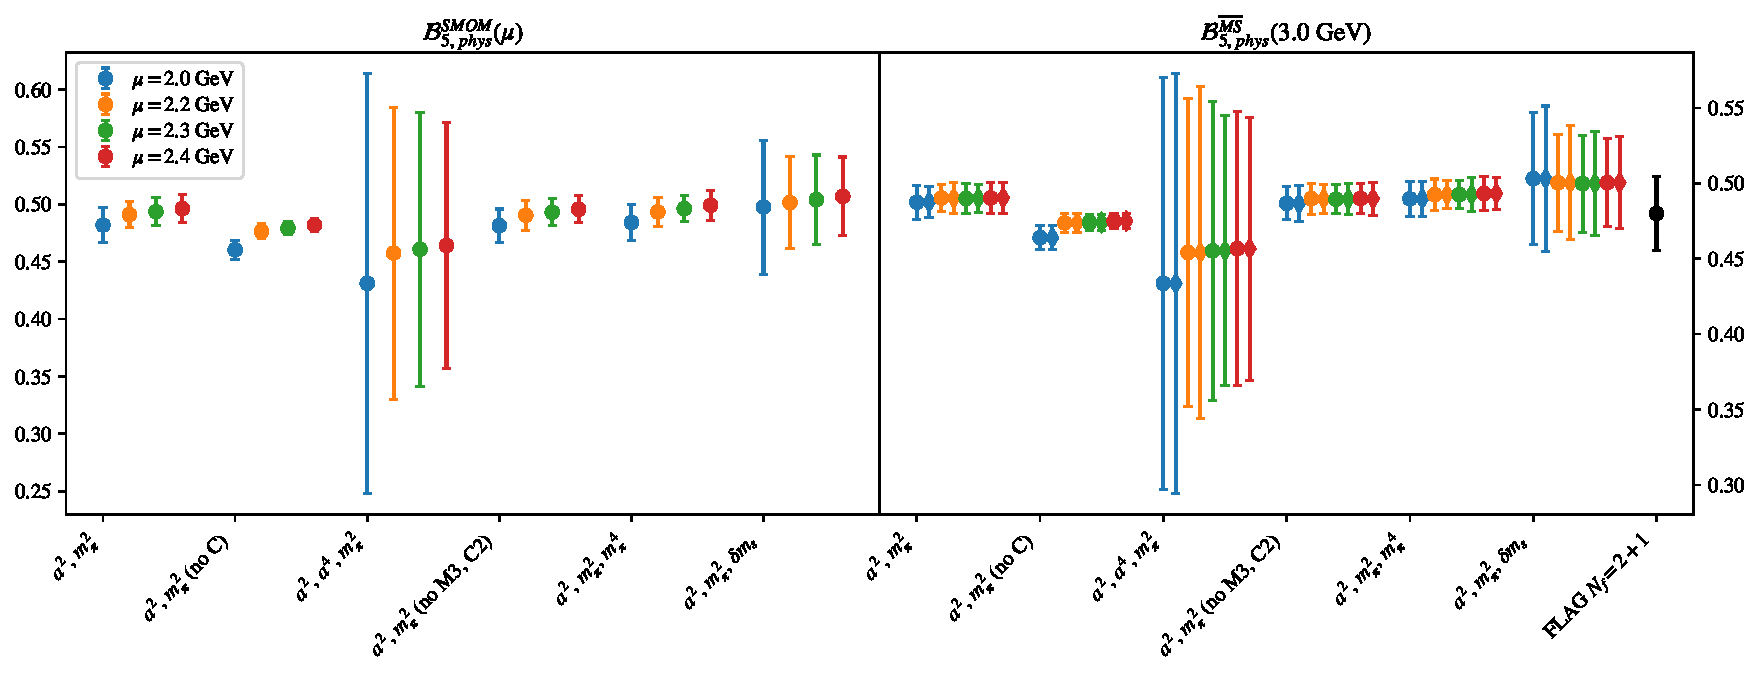
\includegraphics[page=1, width=1.1\textwidth]{TT/SUSY/fit_summary_bag.pdf}
\caption{$\mathcal{B}_{5}$\\(left) $\mathcal{B}_{phys}$ in RI/SMOM scheme from fit variations (fits with $p$-value $<0.05$ marked with ``$\times$"). \\(right) $\mathcal{B}_{phys}$ in $\overline{MS}$ computed using $\mathcal{B}^{\overline{MS}} = R^{\overline{MS}\leftarrow SMOM}(3.0)\sigma_{npt}(3.0,\mu) \mathcal{B}^{SMOM}(\mu)$.}
\end{figure}
\clearpage
\section{$\mathcal{B}_1$}
\begin{table}[h!]
\begin{center}
\begin{tabular}{|c|c|c|c|c|c|c|}
\hline
$\mu$ (GeV) & $a^2$, $m_\pi^2$& $a^2$, $m_\pi^2$ (no C)& $a^2$, $m_\pi^2$, $a^4$& $a^2$, $m_\pi^2$ (no M3, C2)& $a^2$, $m_\pi^2$, $m_\pi^4$& $a^2$, $m_\pi^2$, $\delta m_s$\\
\hline
2.0& \hyperlink{VVpAA/SUSY/bag_a2m2_20.pdf.1}{\textbf{1.4019(28)}: 2.288 (0.043)} & \hyperlink{VVpAA/SUSY/bag_a2m2noC_20.pdf.1}{\textbf{1.436(12)}: 0.226 (0.797)} & \hyperlink{VVpAA/SUSY/bag_a2a4m2_20.pdf.1}{\textbf{1.455(22)}: 1.374 (0.24)} & \hyperlink{VVpAA/SUSY/bag_a2m2mcut_20.pdf.1}{\textbf{1.4055(32)}: 1.926 (0.123)} & \hyperlink{VVpAA/SUSY/bag_a2m2m4_20.pdf.1}{\textbf{1.4046(34)}: 2.309 (0.055)} & \hyperlink{VVpAA/SUSY/bag_a2m2delm_20.pdf.1}{\textbf{1.4027(30)}: 0.771 (0.544)}\\
2.2& \hyperlink{VVpAA/SUSY/bag_a2m2_22.pdf.1}{\textbf{1.3942(28)}: 2.785 (0.016)} & \hyperlink{VVpAA/SUSY/bag_a2m2noC_22.pdf.1}{\textbf{1.431(12)}: 0.357 (0.7)} & \hyperlink{VVpAA/SUSY/bag_a2a4m2_22.pdf.1}{\textbf{1.452(22)}: 1.782 (0.129)} & \hyperlink{VVpAA/SUSY/bag_a2m2mcut_22.pdf.1}{\textbf{1.3983(32)}: 2.262 (0.079)} & \hyperlink{VVpAA/SUSY/bag_a2m2m4_22.pdf.1}{\textbf{1.3971(33)}: 2.61 (0.034)} & \hyperlink{VVpAA/SUSY/bag_a2m2delm_22.pdf.1}{\textbf{1.3951(29)}: 0.976 (0.419)}\\
2.3& \hyperlink{VVpAA/SUSY/bag_a2m2_23.pdf.1}{\textbf{1.3906(28)}: 2.823 (0.015)} & \hyperlink{VVpAA/SUSY/bag_a2m2noC_23.pdf.1}{\textbf{1.428(12)}: 0.354 (0.702)} & \hyperlink{VVpAA/SUSY/bag_a2a4m2_23.pdf.1}{\textbf{1.449(22)}: 1.774 (0.131)} & \hyperlink{VVpAA/SUSY/bag_a2m2mcut_23.pdf.1}{\textbf{1.3950(31)}: 2.367 (0.069)} & \hyperlink{VVpAA/SUSY/bag_a2m2m4_23.pdf.1}{\textbf{1.3939(33)}: 2.751 (0.027)} & \hyperlink{VVpAA/SUSY/bag_a2m2delm_23.pdf.1}{\textbf{1.3919(29)}: 0.995 (0.409)}\\
2.4& \hyperlink{VVpAA/SUSY/bag_a2m2_24.pdf.1}{\textbf{1.3879(28)}: 2.926 (0.012)} & \hyperlink{VVpAA/SUSY/bag_a2m2noC_24.pdf.1}{\textbf{1.425(12)}: 0.387 (0.679)} & \hyperlink{VVpAA/SUSY/bag_a2a4m2_24.pdf.1}{\textbf{1.447(22)}: 1.879 (0.111)} & \hyperlink{VVpAA/SUSY/bag_a2m2mcut_24.pdf.1}{\textbf{1.3923(31)}: 2.395 (0.066)} & \hyperlink{VVpAA/SUSY/bag_a2m2m4_24.pdf.1}{\textbf{1.3910(33)}: 2.746 (0.027)} & \hyperlink{VVpAA/SUSY/bag_a2m2delm_24.pdf.1}{\textbf{1.3891(29)}: 1.03 (0.39)}\\
\hline
\end{tabular}
\caption{Physical point value from chiral and continuum extrapolation at renormalisation scale $\mu$. Entries are \textbf{value(error)}: $\chi^2/\text{DOF}$ ($p$-value).}
\end{center}
\end{table}
\begin{table}[h!]
\begin{center}
\begin{tabular}{|c c|c|c|c|c|c|c|}
\hline
$\mu$ (GeV) &  & $a^2$, $m_\pi^2$& $a^2$, $m_\pi^2$ (no C)& $a^2$, $m_\pi^2$, $a^4$& $a^2$, $m_\pi^2$ (no M3, C2)& $a^2$, $m_\pi^2$, $m_\pi^4$& $a^2$, $m_\pi^2$, $\delta m_s$\\
\hline
\multirow{3}{0.5in}{2.0} & $\alpha$ & 0.140(10)& -0.054(76)& -0.35(20)& 0.129(11)& 0.132(11)& 0.141(10)\\
 & $\beta$ & 0.00374(20)& 0.00335(38)& 0.00402(23)& 0.00316(32)& 0.0021(10)& 0.00501(50)\\
 & $\gamma$ &  &  & 1.00(42)&  & 0.000147(92)& -0.050(18)\\
\hline
\multirow{3}{0.5in}{2.2} & $\alpha$ & 0.146(10)& -0.062(76)& -0.38(20)& 0.133(11)& 0.137(11)& 0.147(10)\\
 & $\beta$ & 0.00372(20)& 0.00329(39)& 0.00401(23)& 0.00307(33)& 0.0019(10)& 0.00508(51)\\
 & $\gamma$ &  &  & 1.08(41)&  & 0.000162(91)& -0.053(18)\\
\hline
\multirow{3}{0.5in}{2.3} & $\alpha$ & 0.148(10)& -0.064(76)& -0.38(20)& 0.135(11)& 0.139(11)& 0.149(10)\\
 & $\beta$ & 0.00373(20)& 0.00327(39)& 0.00402(23)& 0.00306(32)& 0.0019(10)& 0.00511(50)\\
 & $\gamma$ &  &  & 1.08(41)&  & 0.000165(92)& -0.054(18)\\
\hline
\multirow{3}{0.5in}{2.4} & $\alpha$ & 0.149(10)& -0.064(76)& -0.39(20)& 0.135(11)& 0.140(11)& 0.150(10)\\
 & $\beta$ & 0.00373(20)& 0.00327(38)& 0.00404(22)& 0.00306(32)& 0.0019(10)& 0.00513(50)\\
 & $\gamma$ &  &  & 1.10(41)&  & 0.000167(90)& -0.054(18)\\
\hline
\end{tabular}
\caption{Fit values of coefficients in $Q = Q_{phys} + \mathbf{\alpha} a^2 + \mathbf{\beta}\left(\frac{m_\pi^2}{f_\pi^2}-\frac{m_{\pi,PDG}^2}{f_\pi^2}\right) + \gamma(\ldots)$}
\end{center}
\end{table}
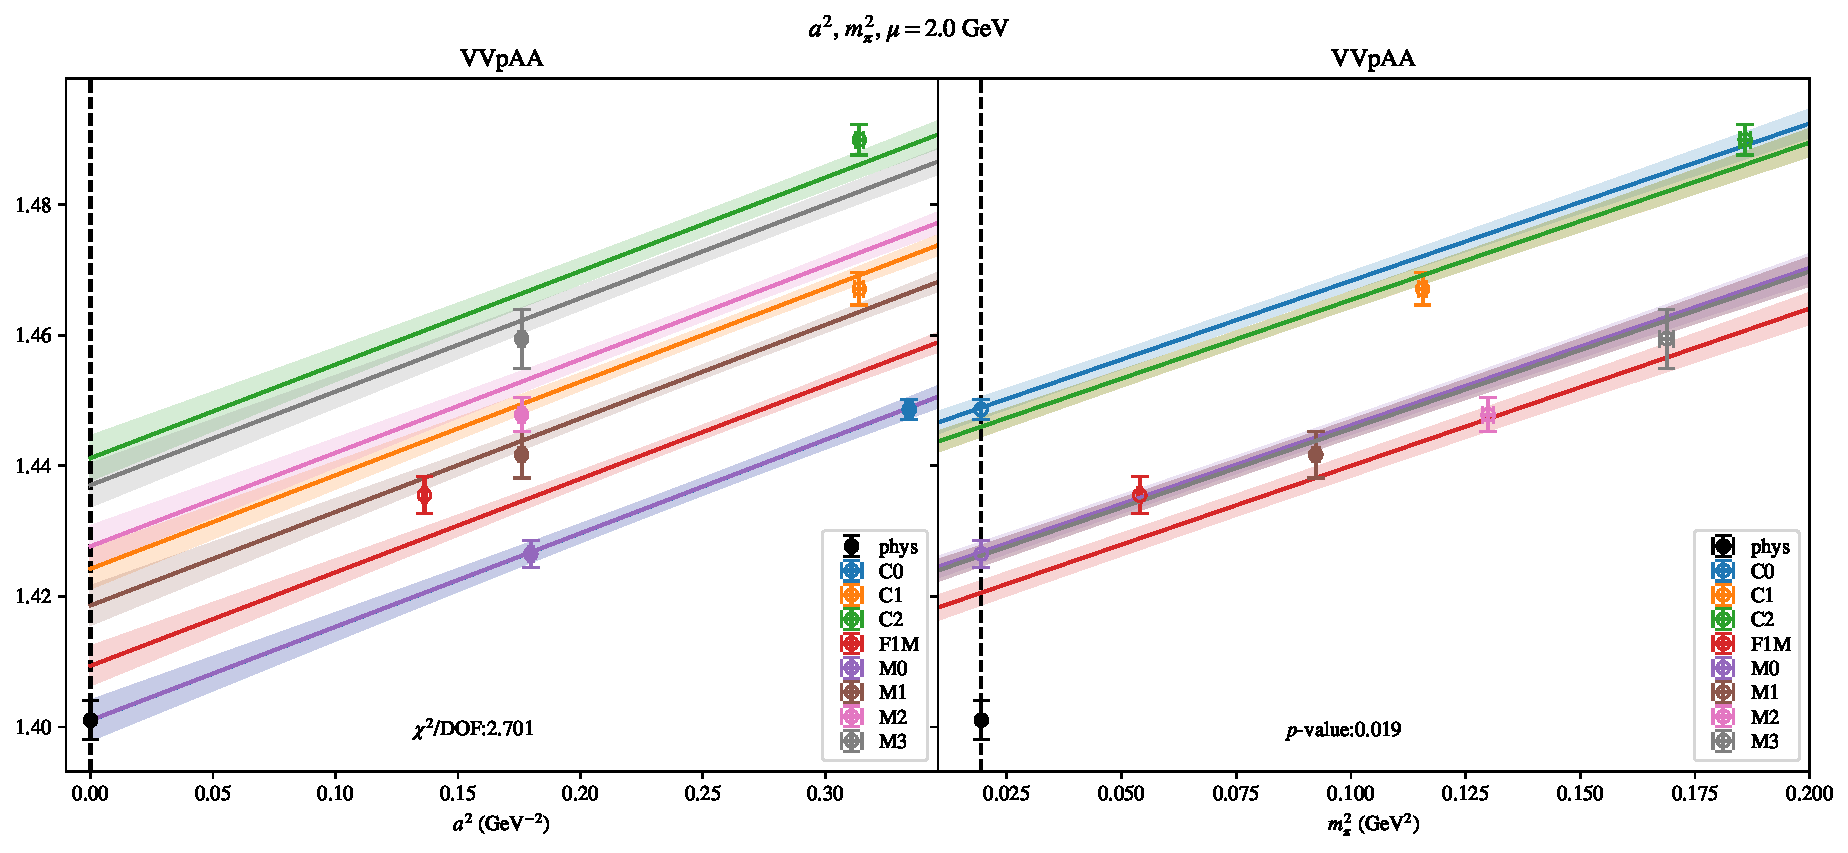
\includepdf[link, pages=-]{VVpAA/SUSY/bag_a2m2_20.pdf}
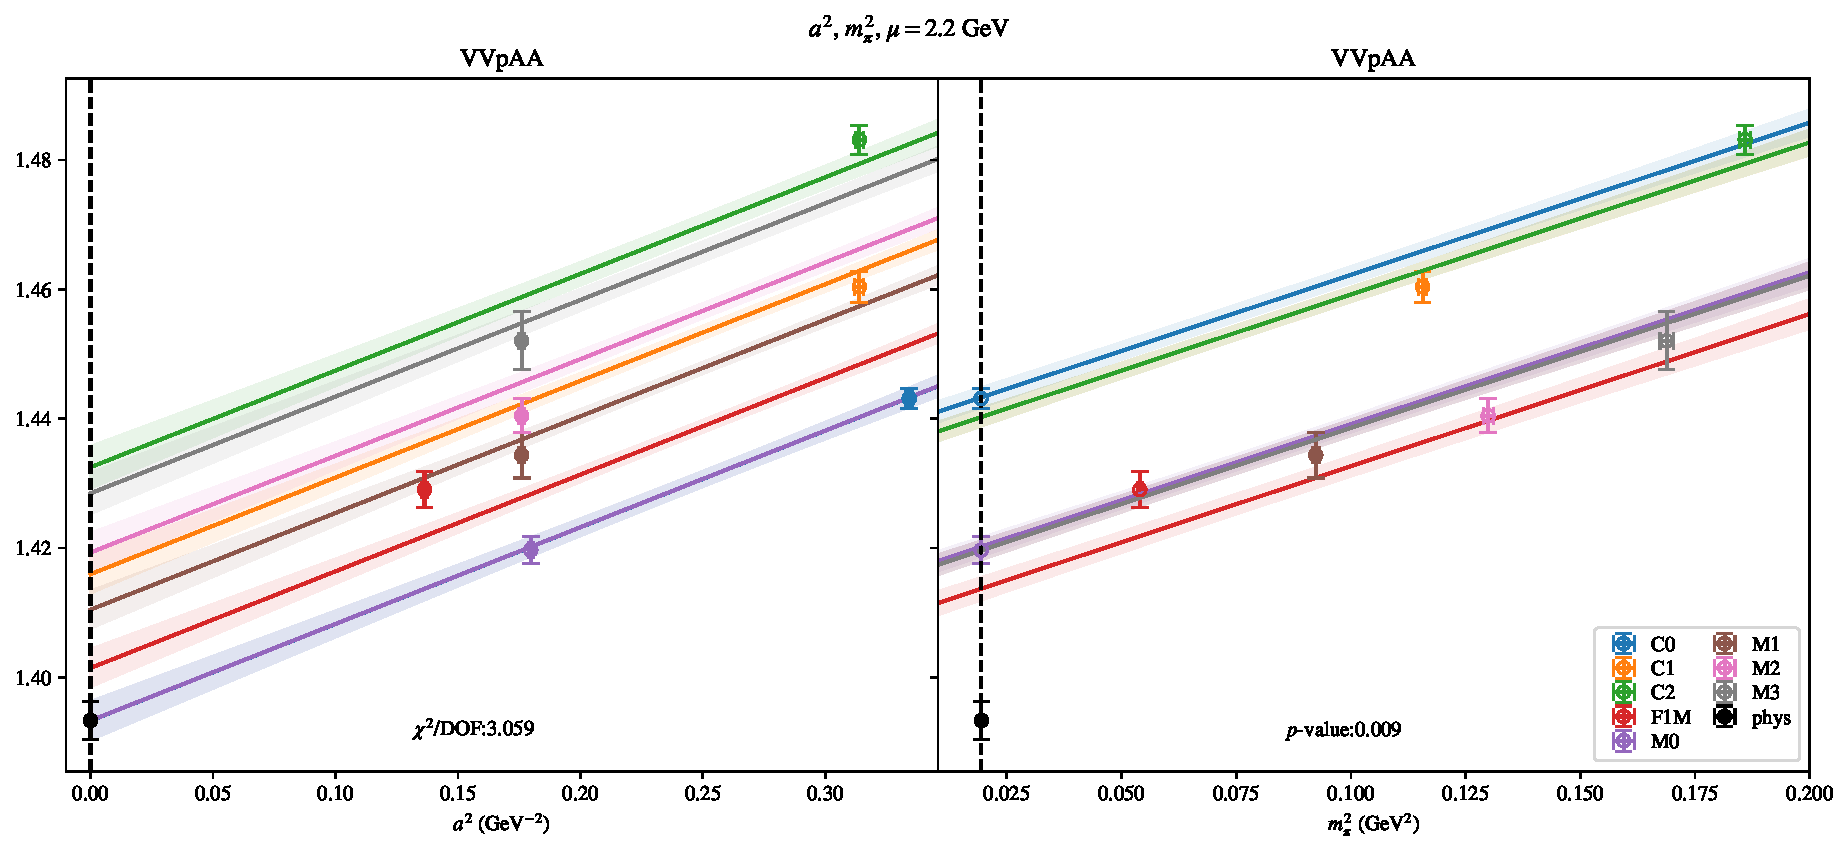
\includepdf[link, pages=-]{VVpAA/SUSY/bag_a2m2_22.pdf}
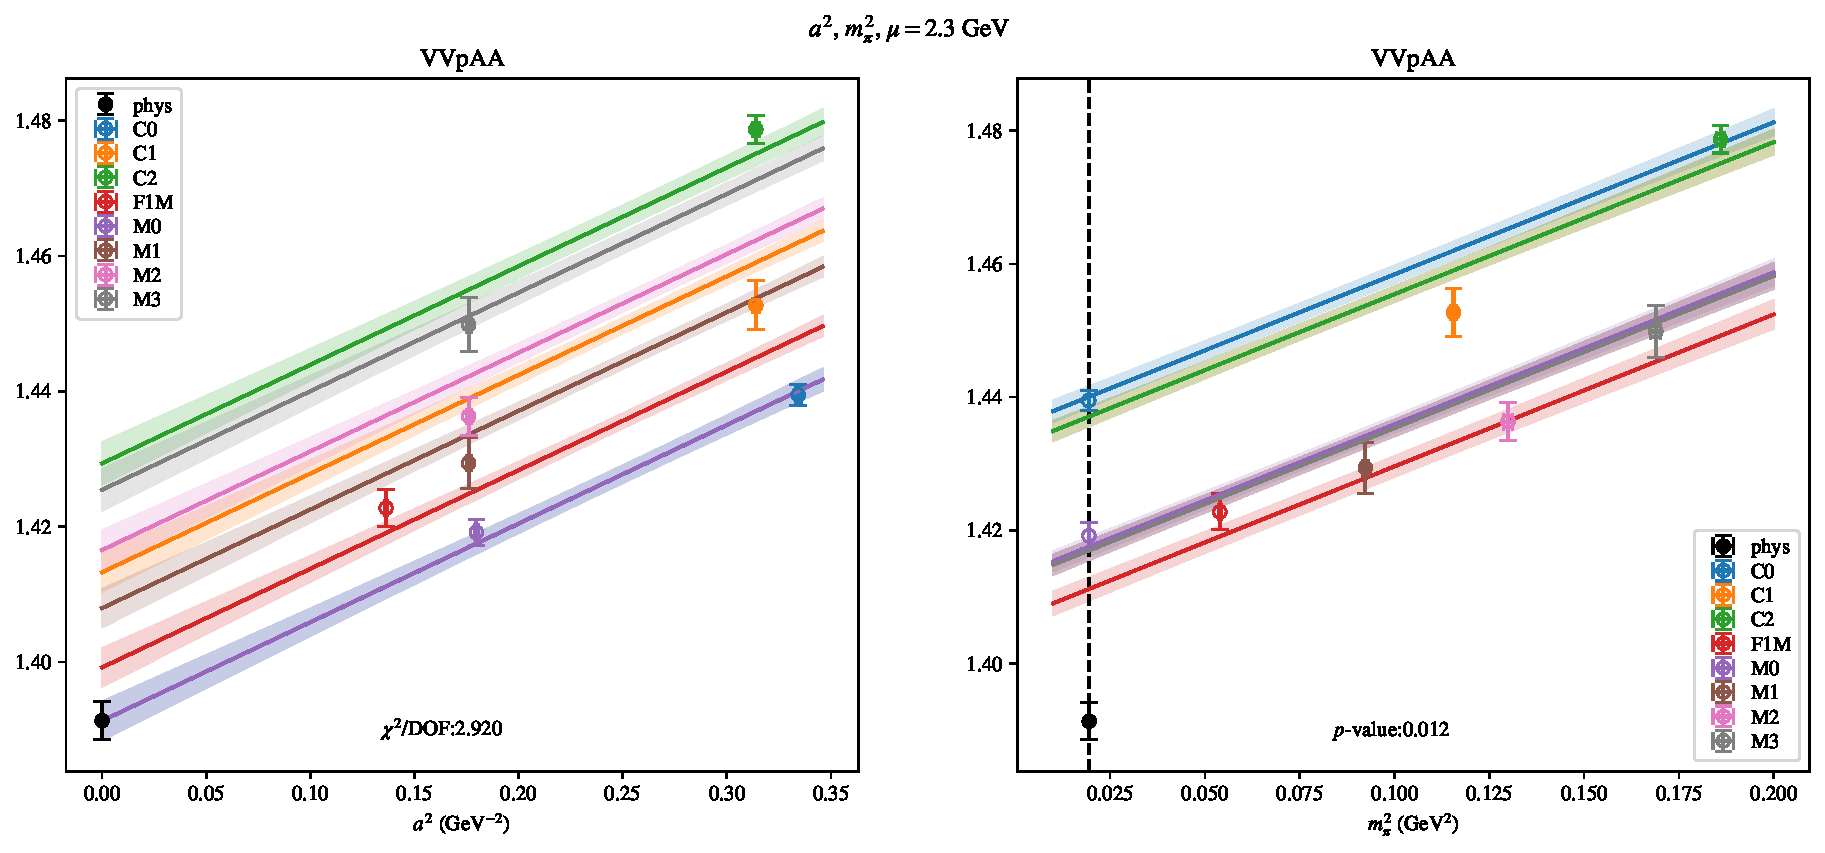
\includepdf[link, pages=-]{VVpAA/SUSY/bag_a2m2_23.pdf}
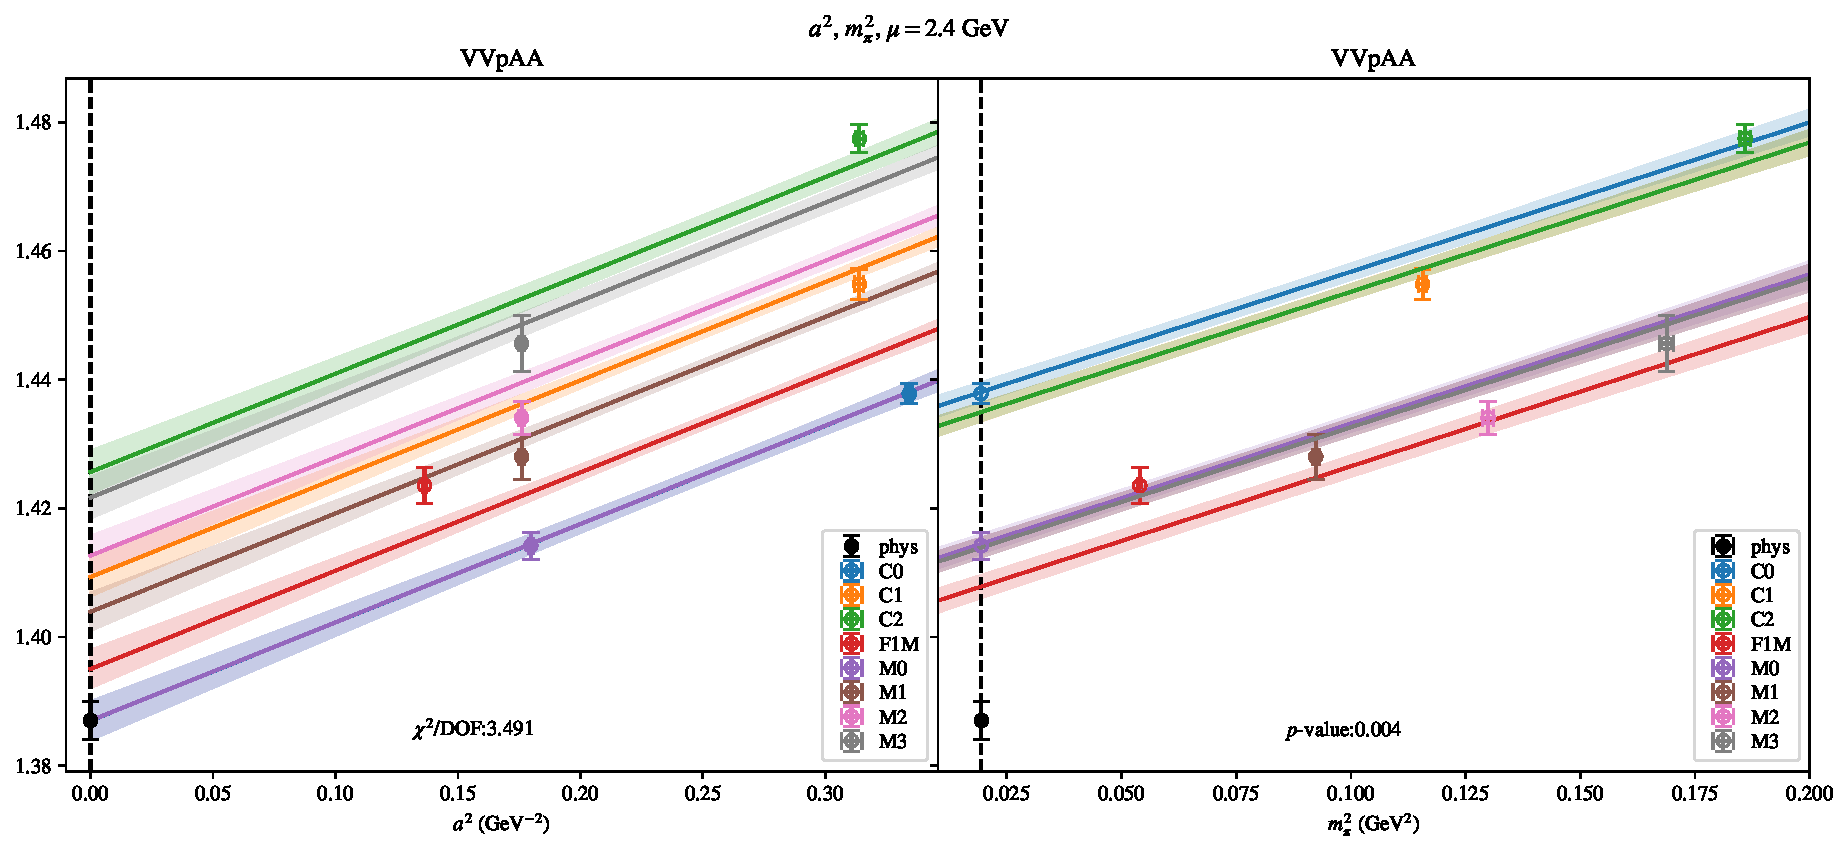
\includepdf[link, pages=-]{VVpAA/SUSY/bag_a2m2_24.pdf}
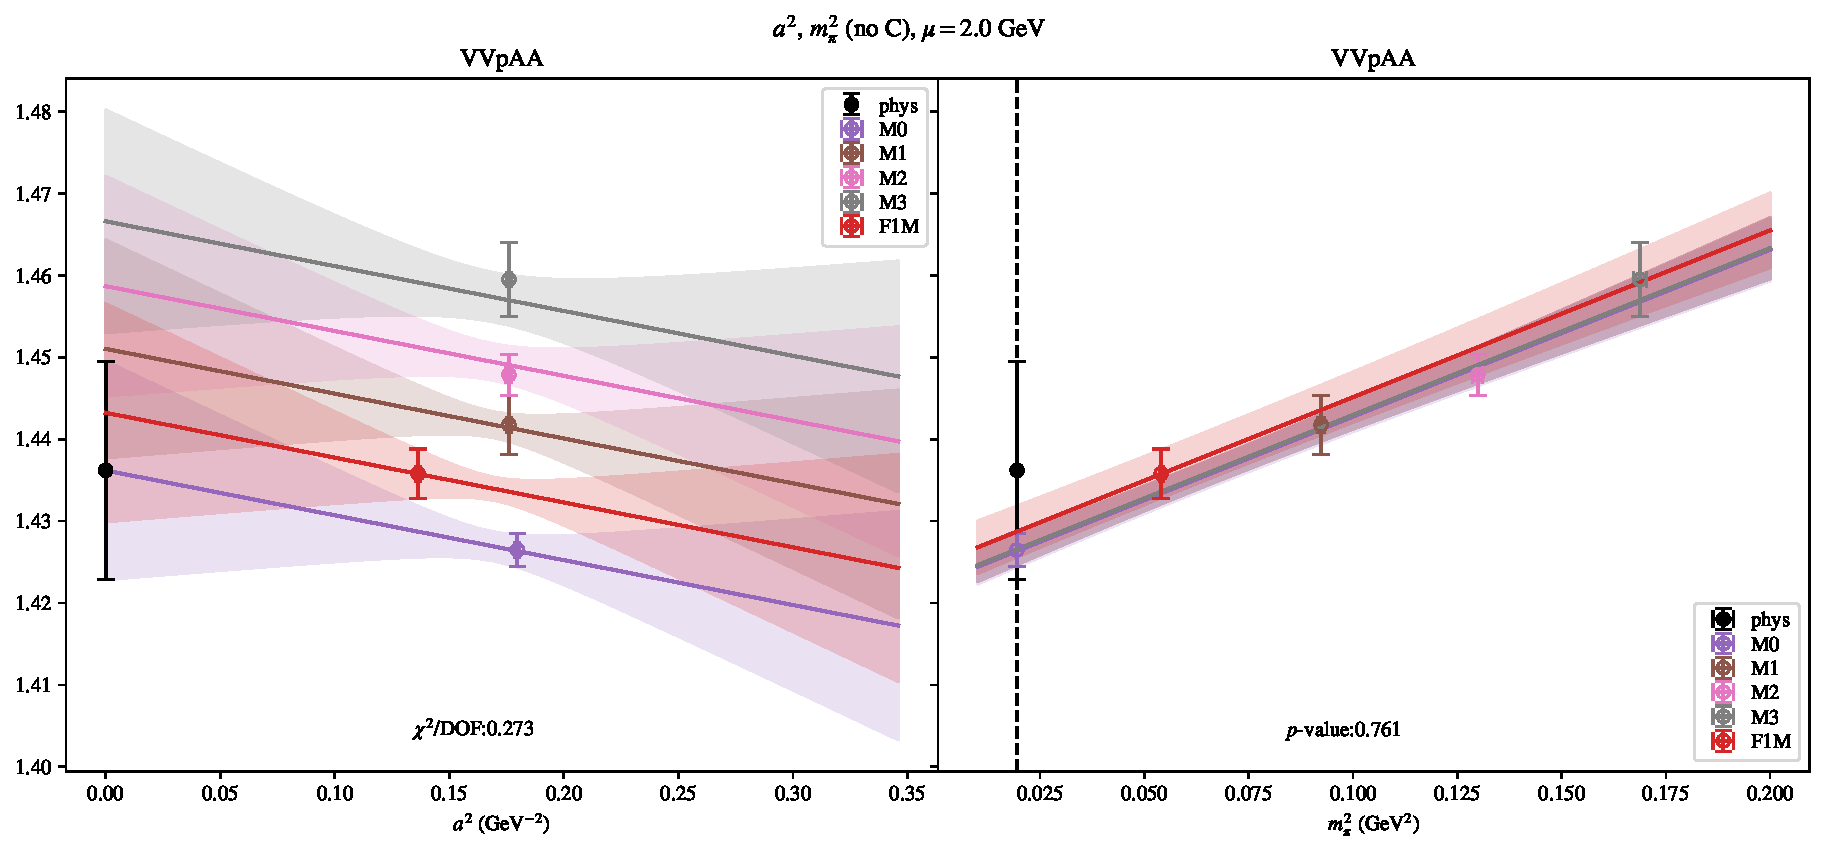
\includepdf[link, pages=-]{VVpAA/SUSY/bag_a2m2noC_20.pdf}
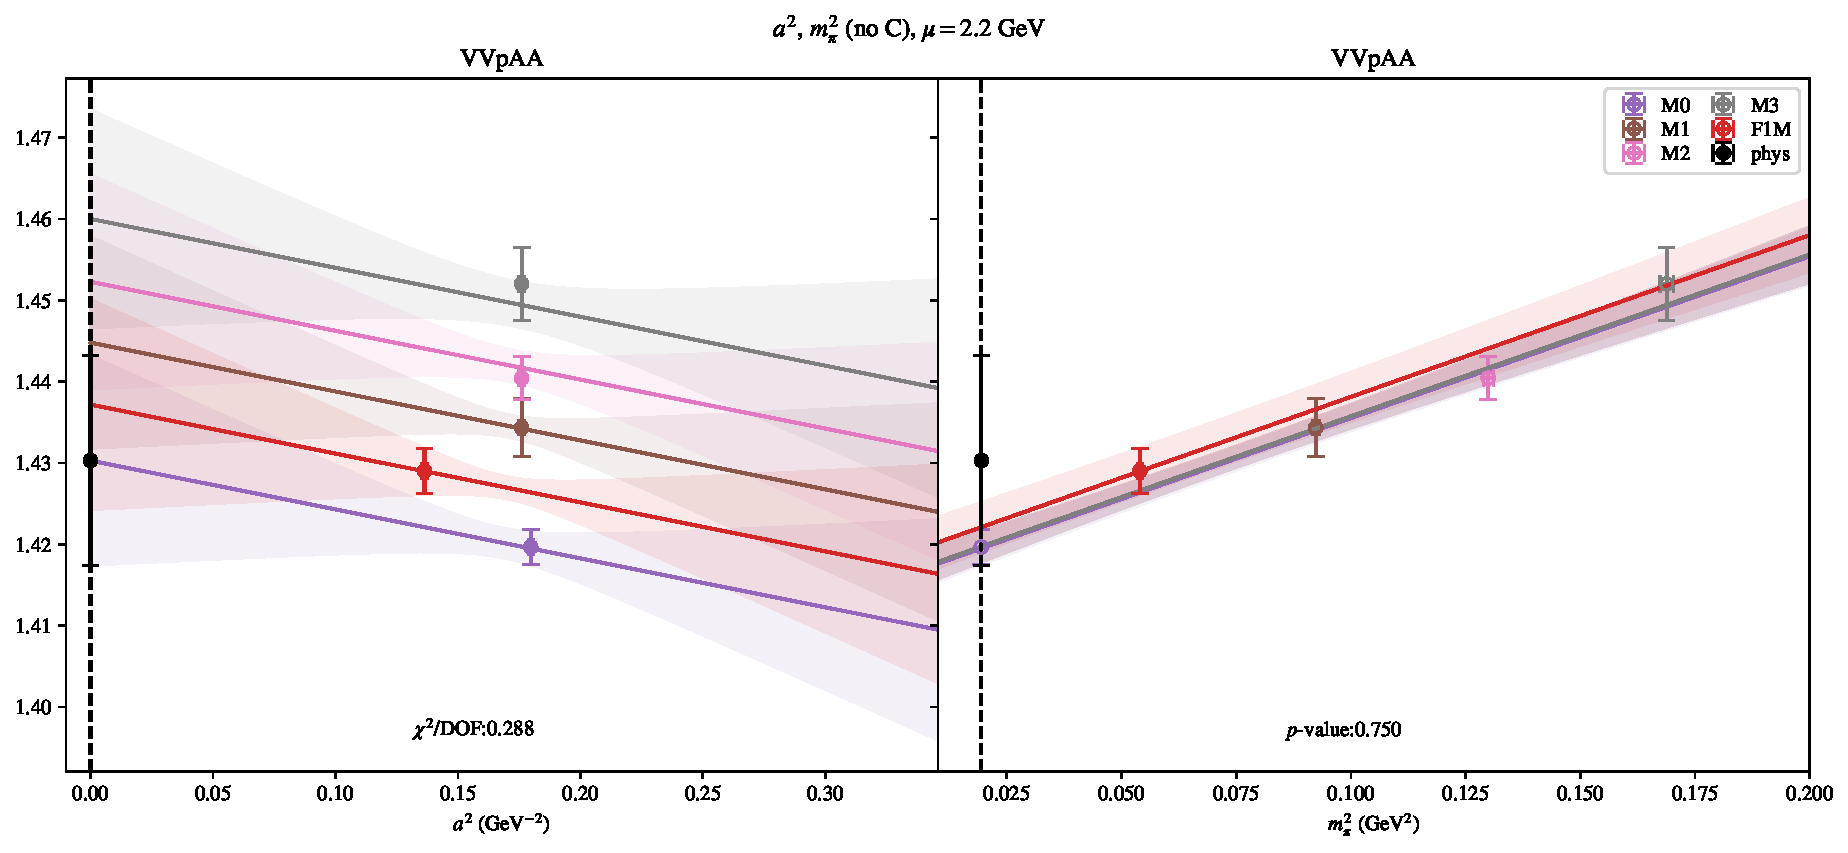
\includepdf[link, pages=-]{VVpAA/SUSY/bag_a2m2noC_22.pdf}
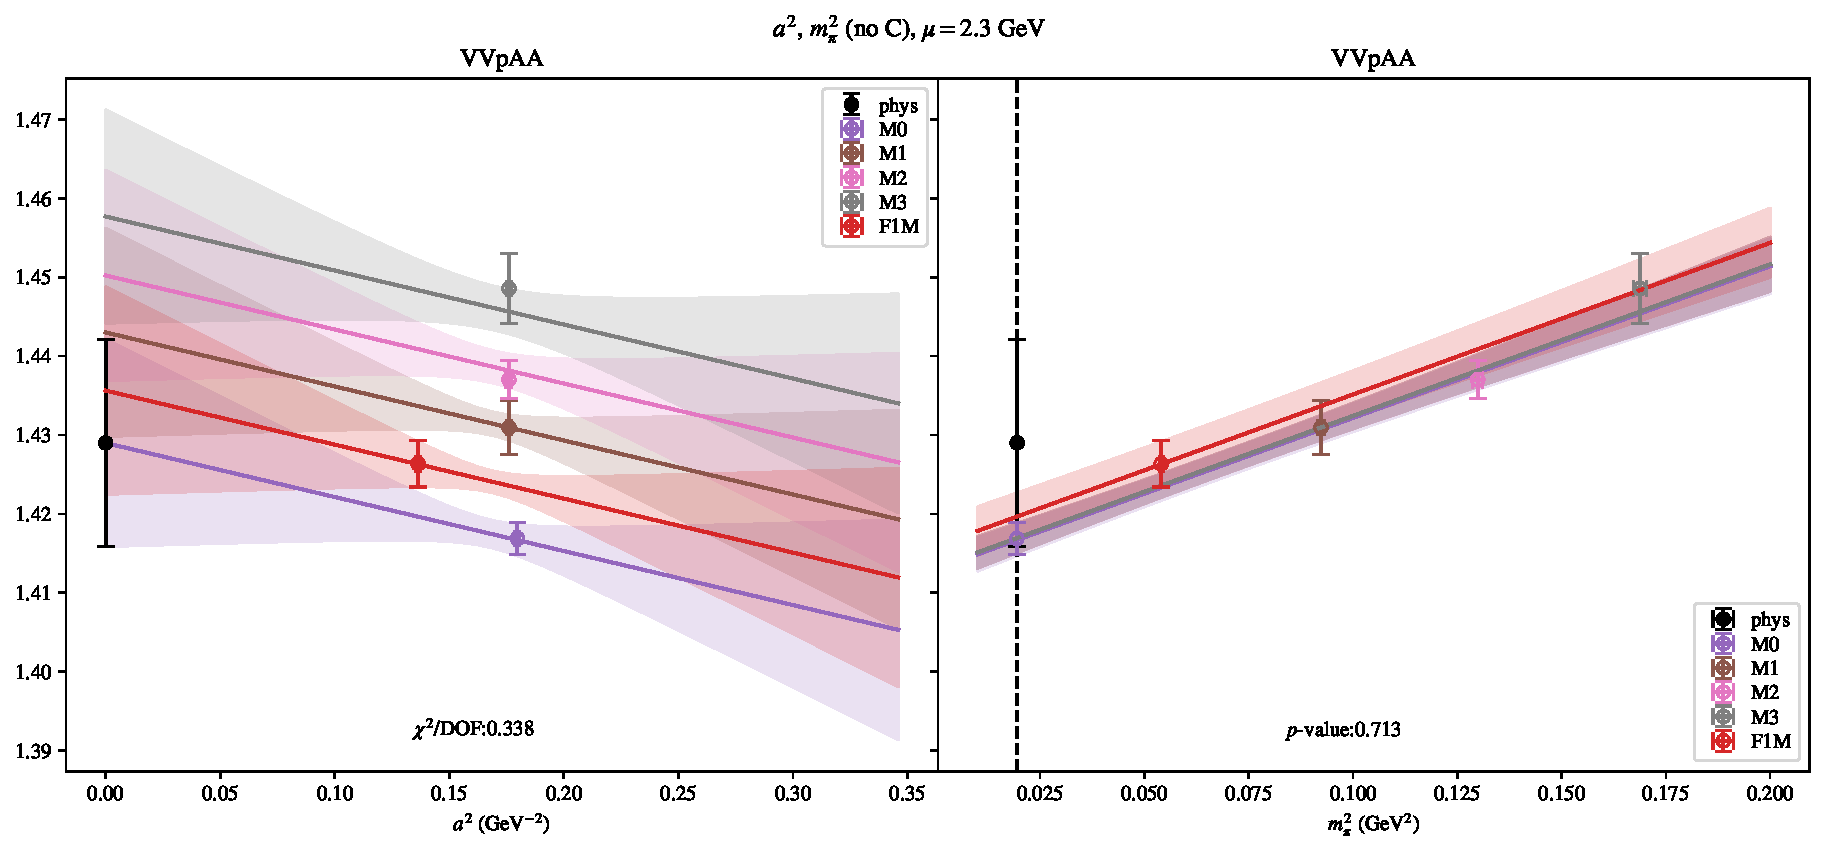
\includepdf[link, pages=-]{VVpAA/SUSY/bag_a2m2noC_23.pdf}
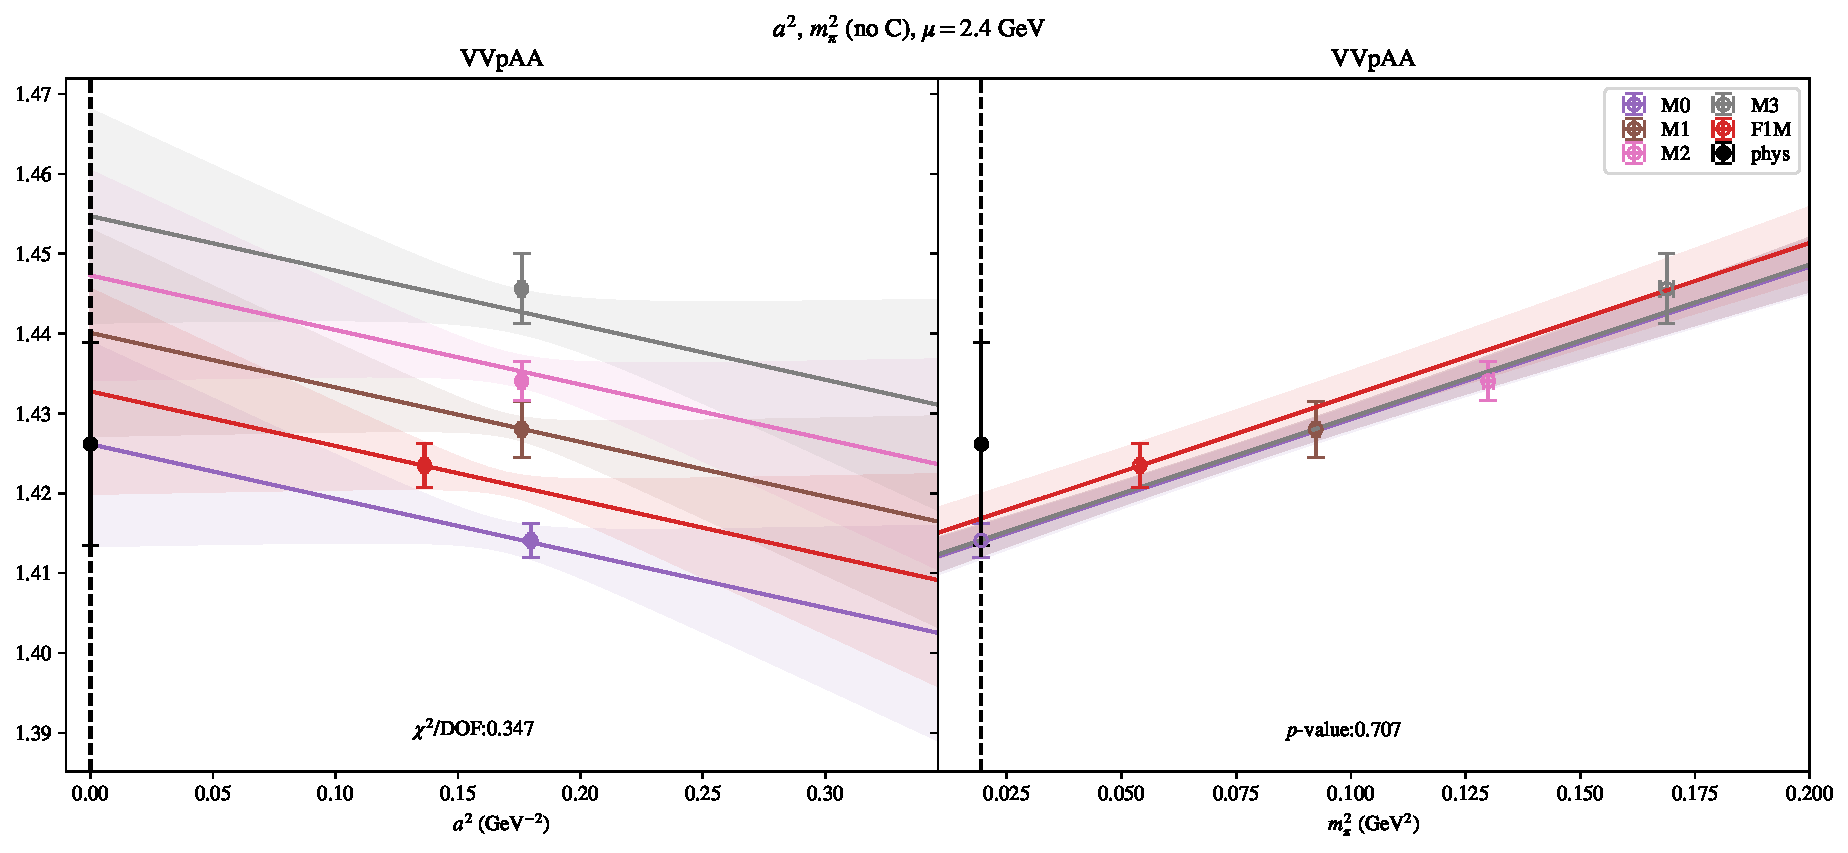
\includepdf[link, pages=-]{VVpAA/SUSY/bag_a2m2noC_24.pdf}
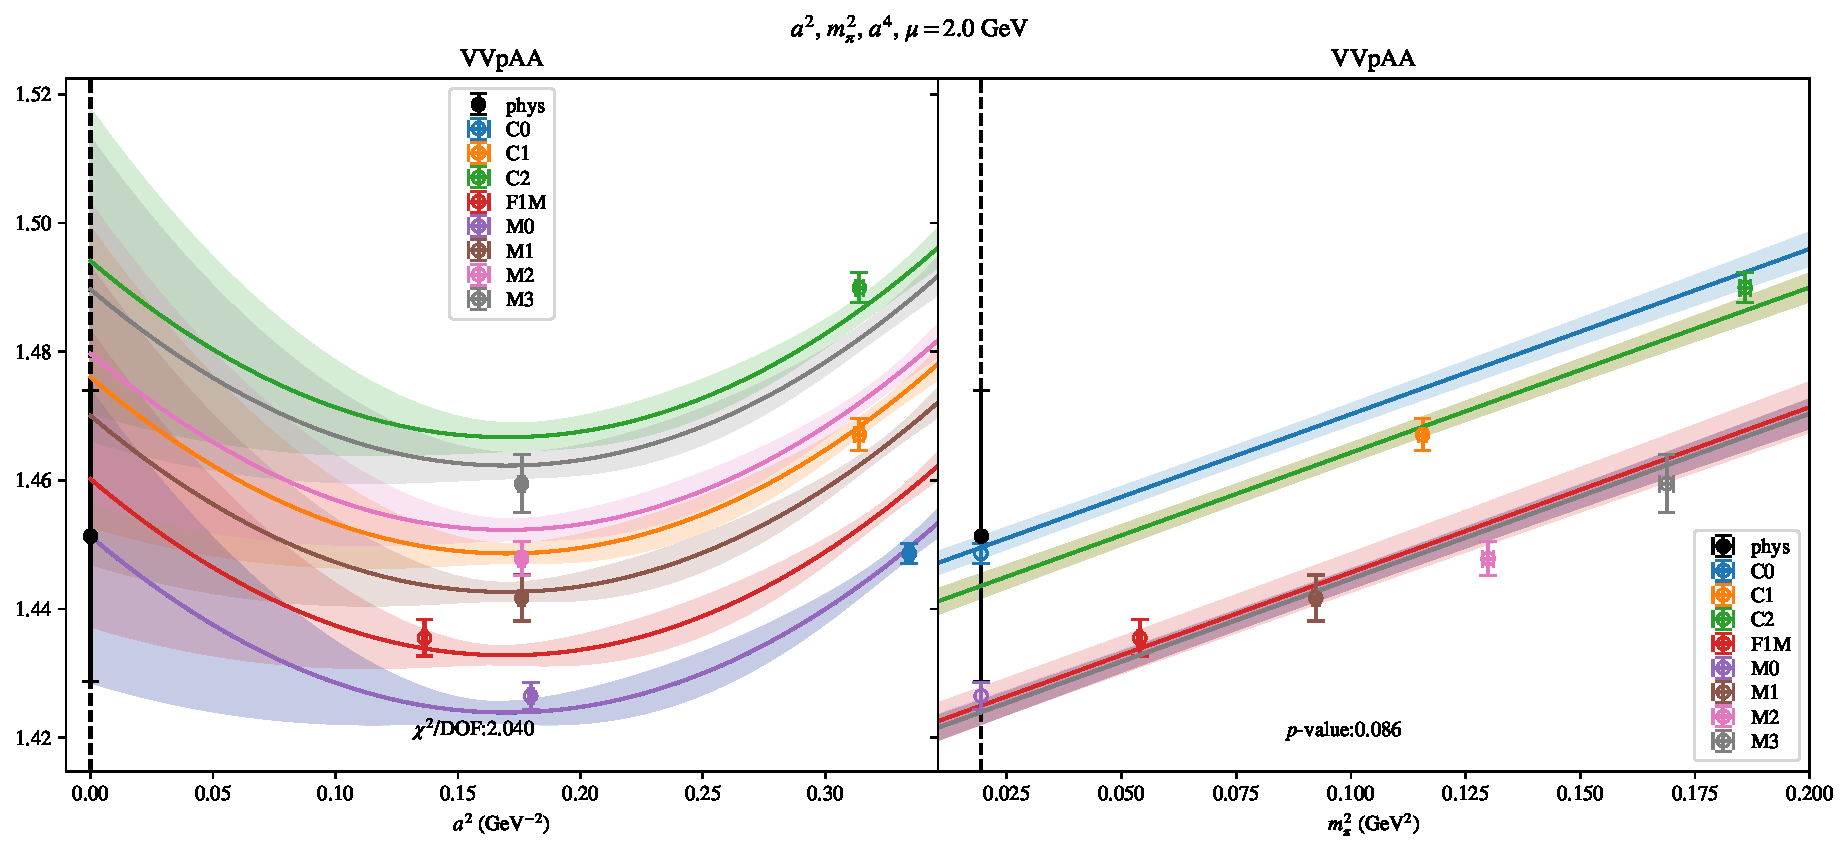
\includepdf[link, pages=-]{VVpAA/SUSY/bag_a2a4m2_20.pdf}
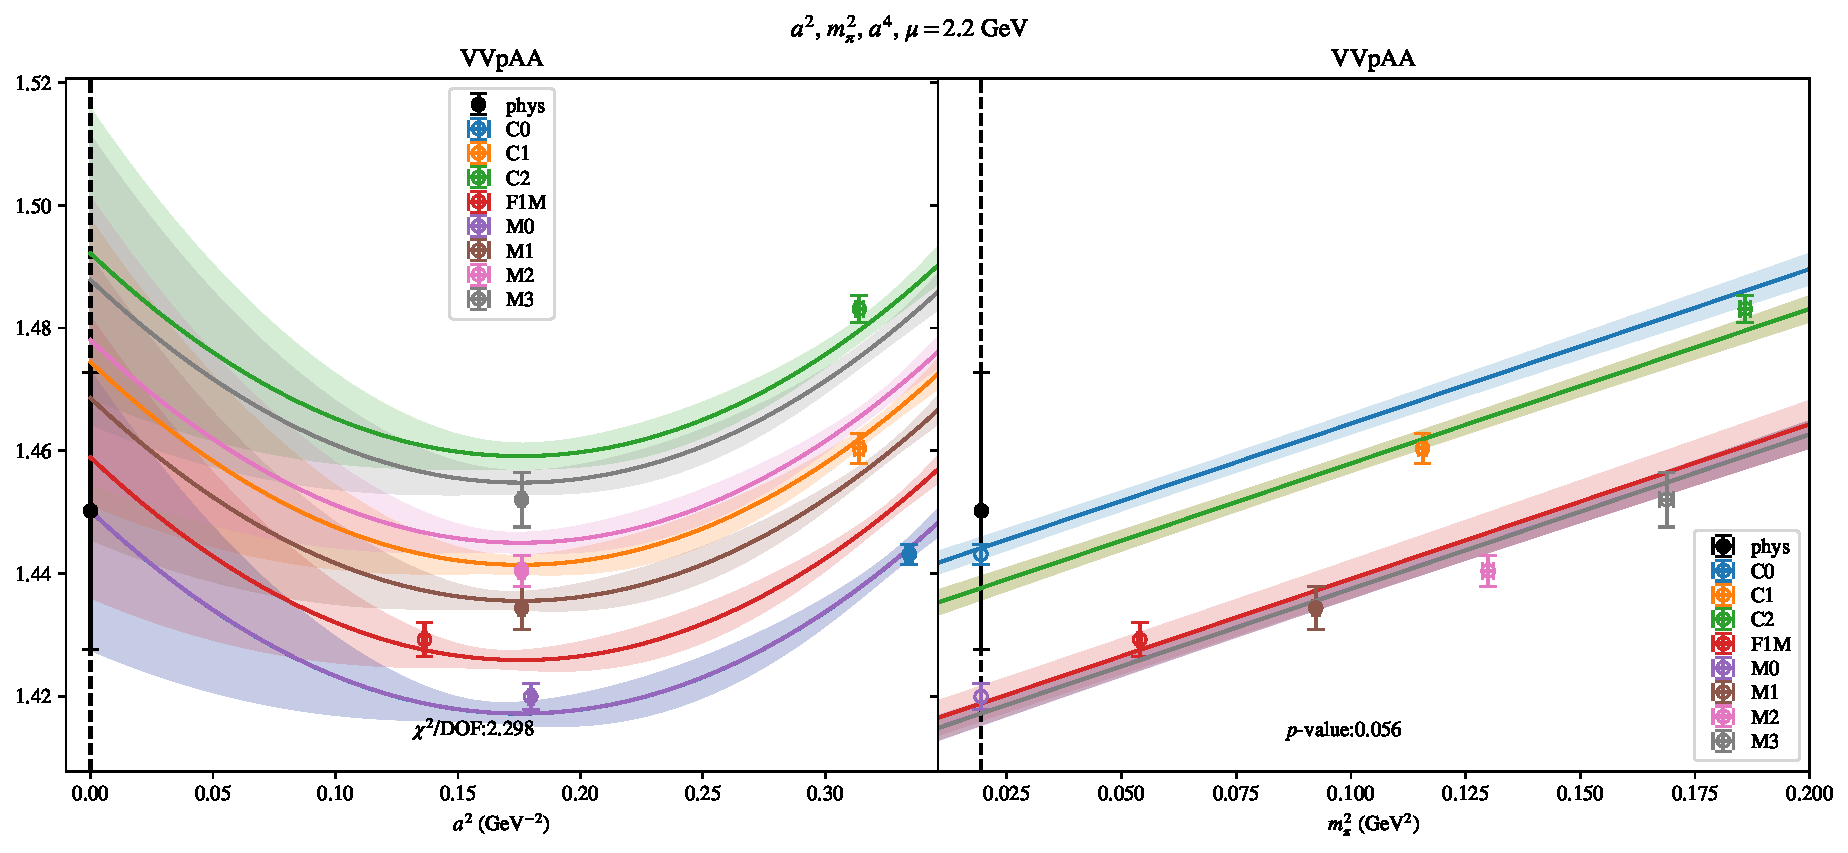
\includepdf[link, pages=-]{VVpAA/SUSY/bag_a2a4m2_22.pdf}
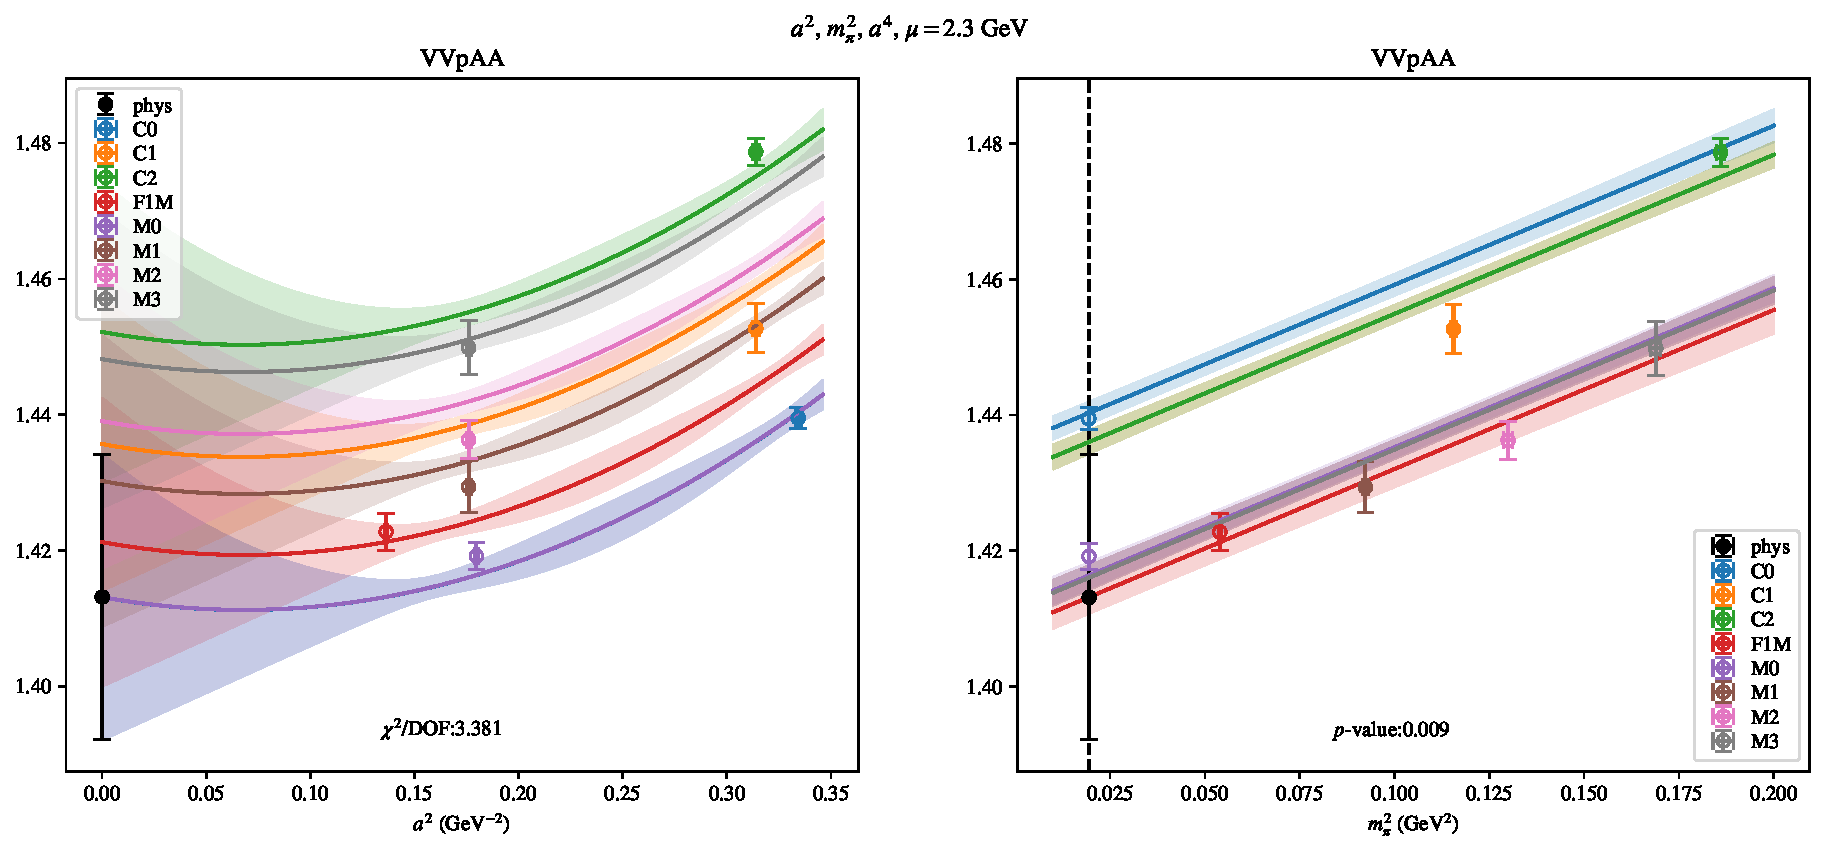
\includepdf[link, pages=-]{VVpAA/SUSY/bag_a2a4m2_23.pdf}
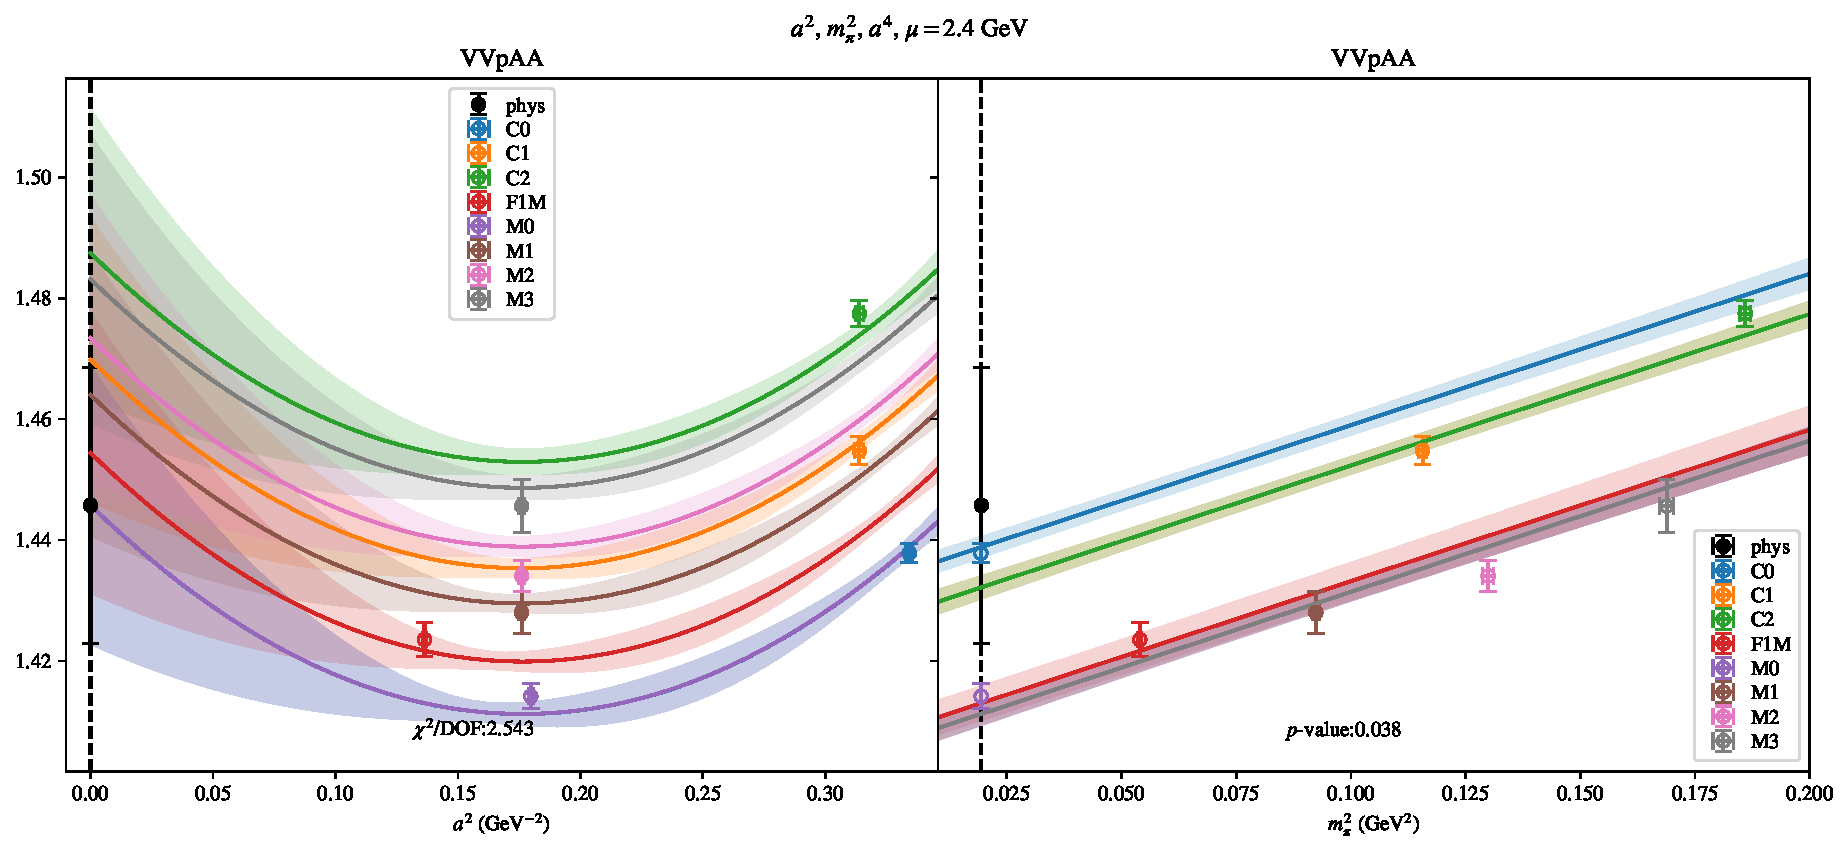
\includepdf[link, pages=-]{VVpAA/SUSY/bag_a2a4m2_24.pdf}
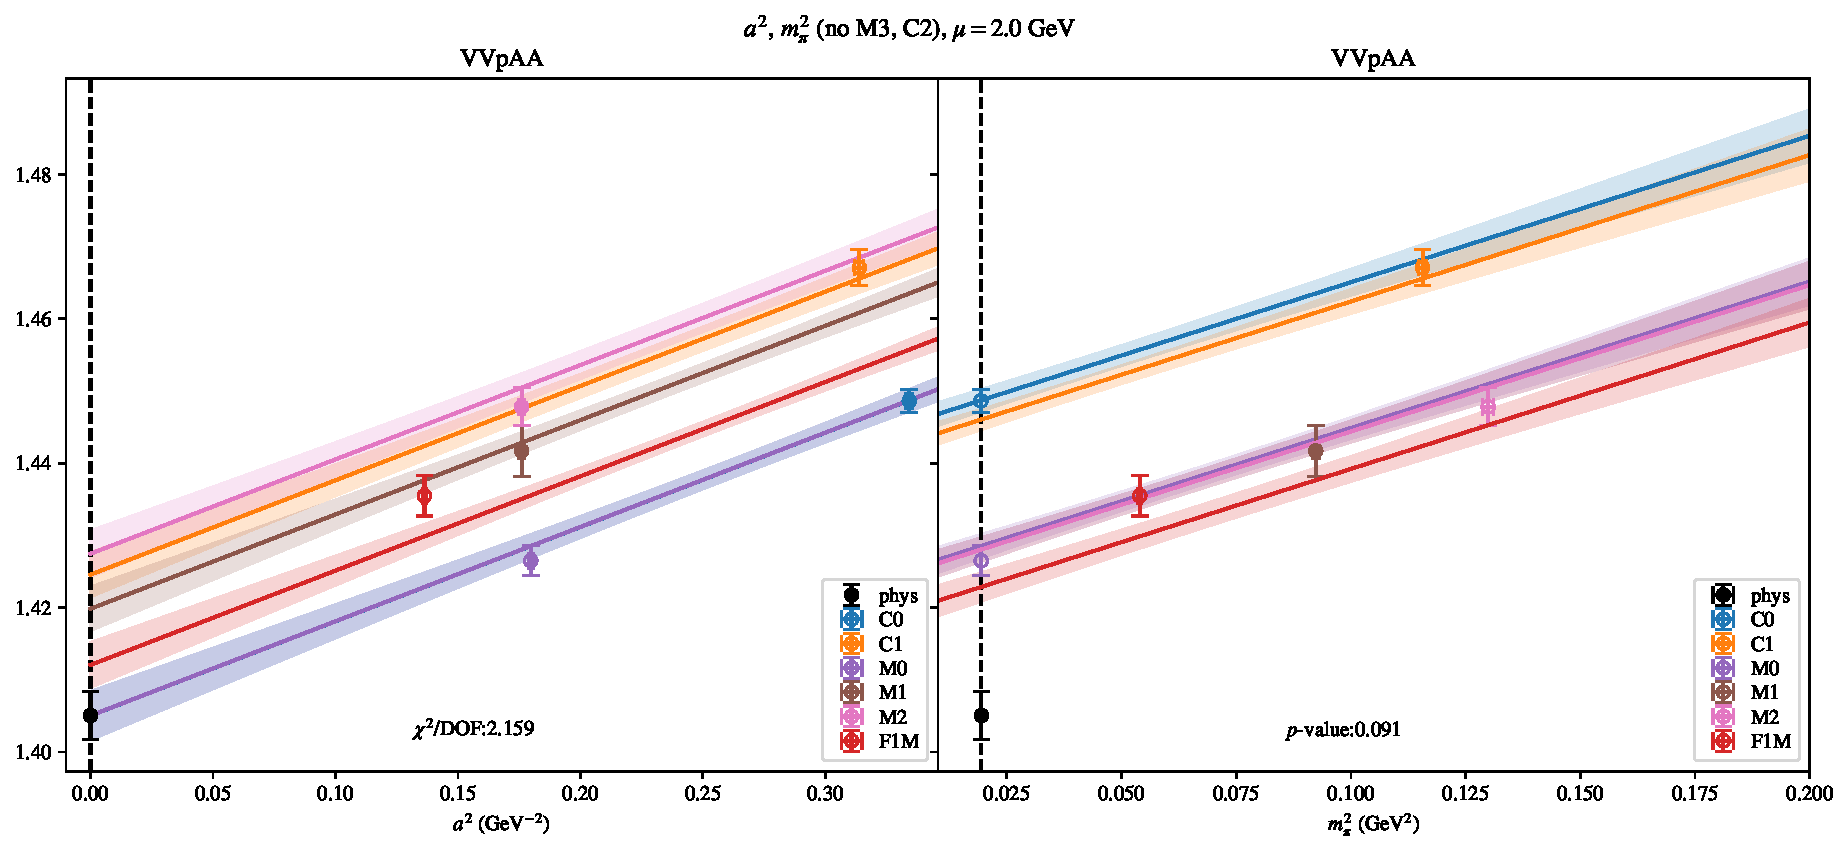
\includepdf[link, pages=-]{VVpAA/SUSY/bag_a2m2mcut_20.pdf}
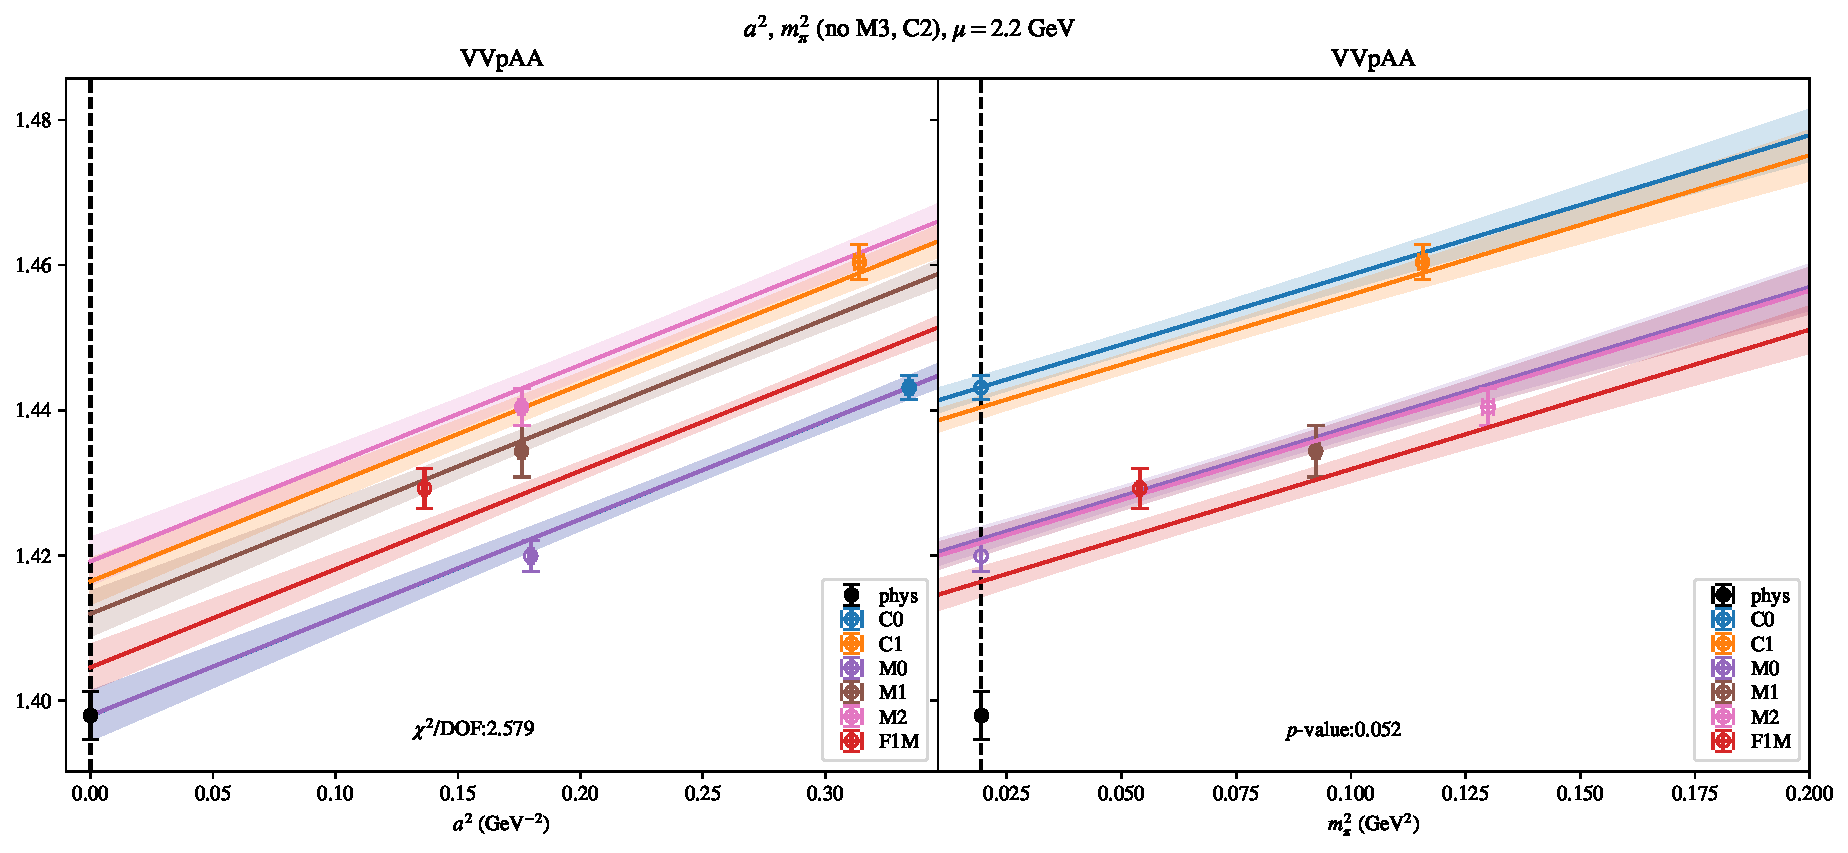
\includepdf[link, pages=-]{VVpAA/SUSY/bag_a2m2mcut_22.pdf}
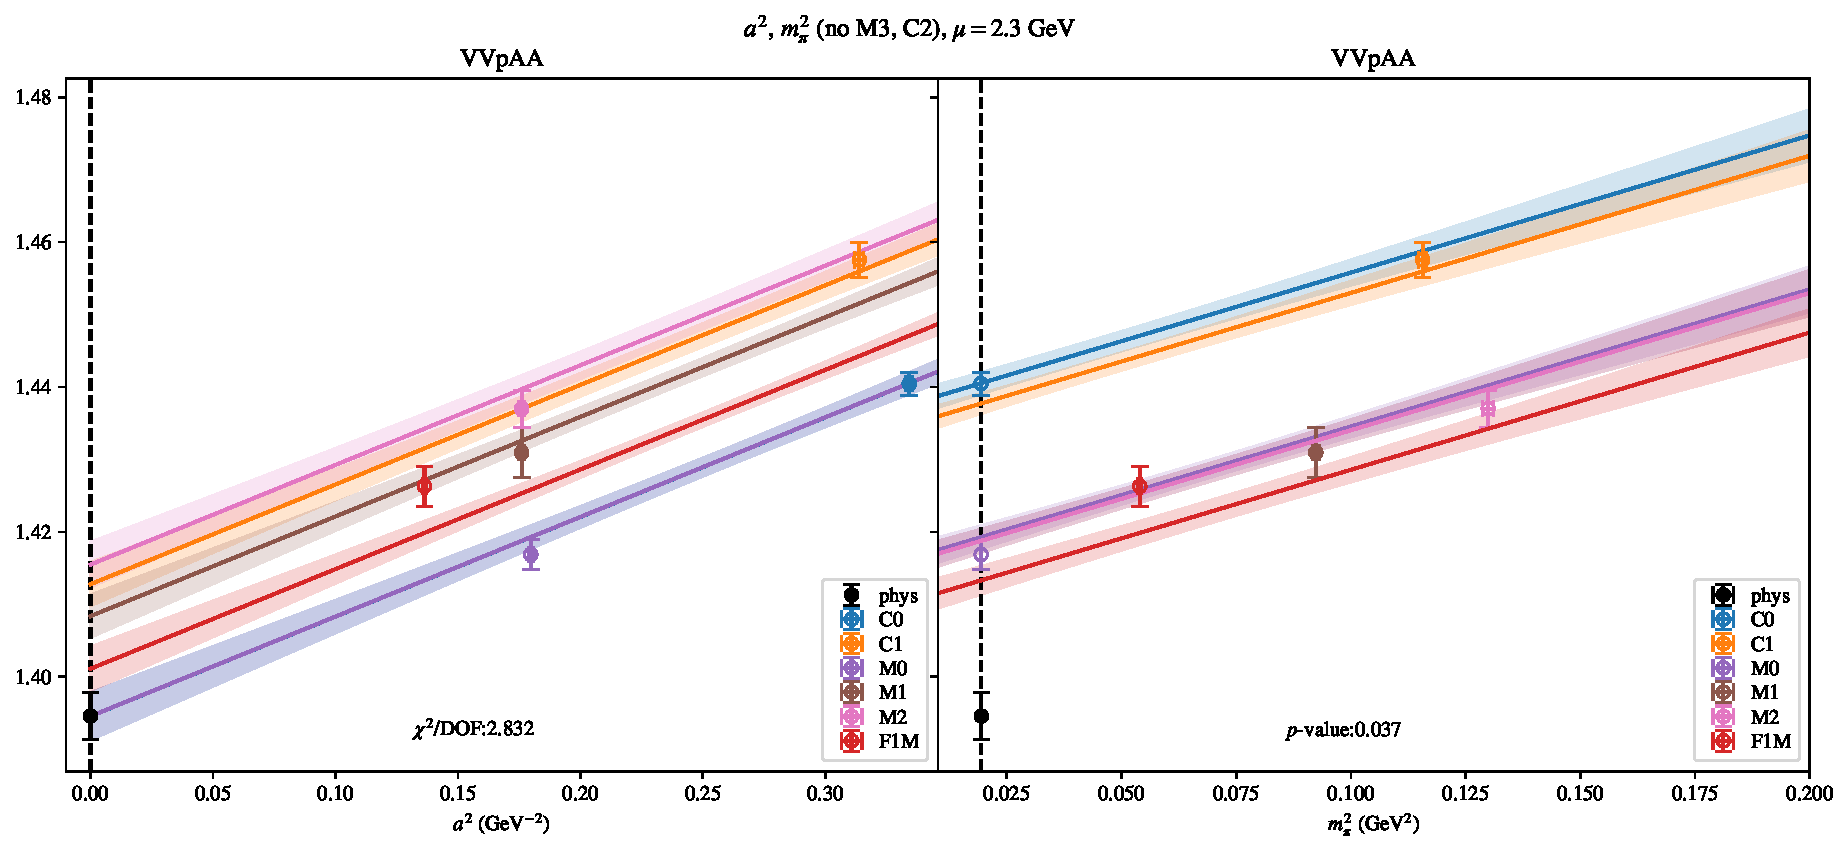
\includepdf[link, pages=-]{VVpAA/SUSY/bag_a2m2mcut_23.pdf}
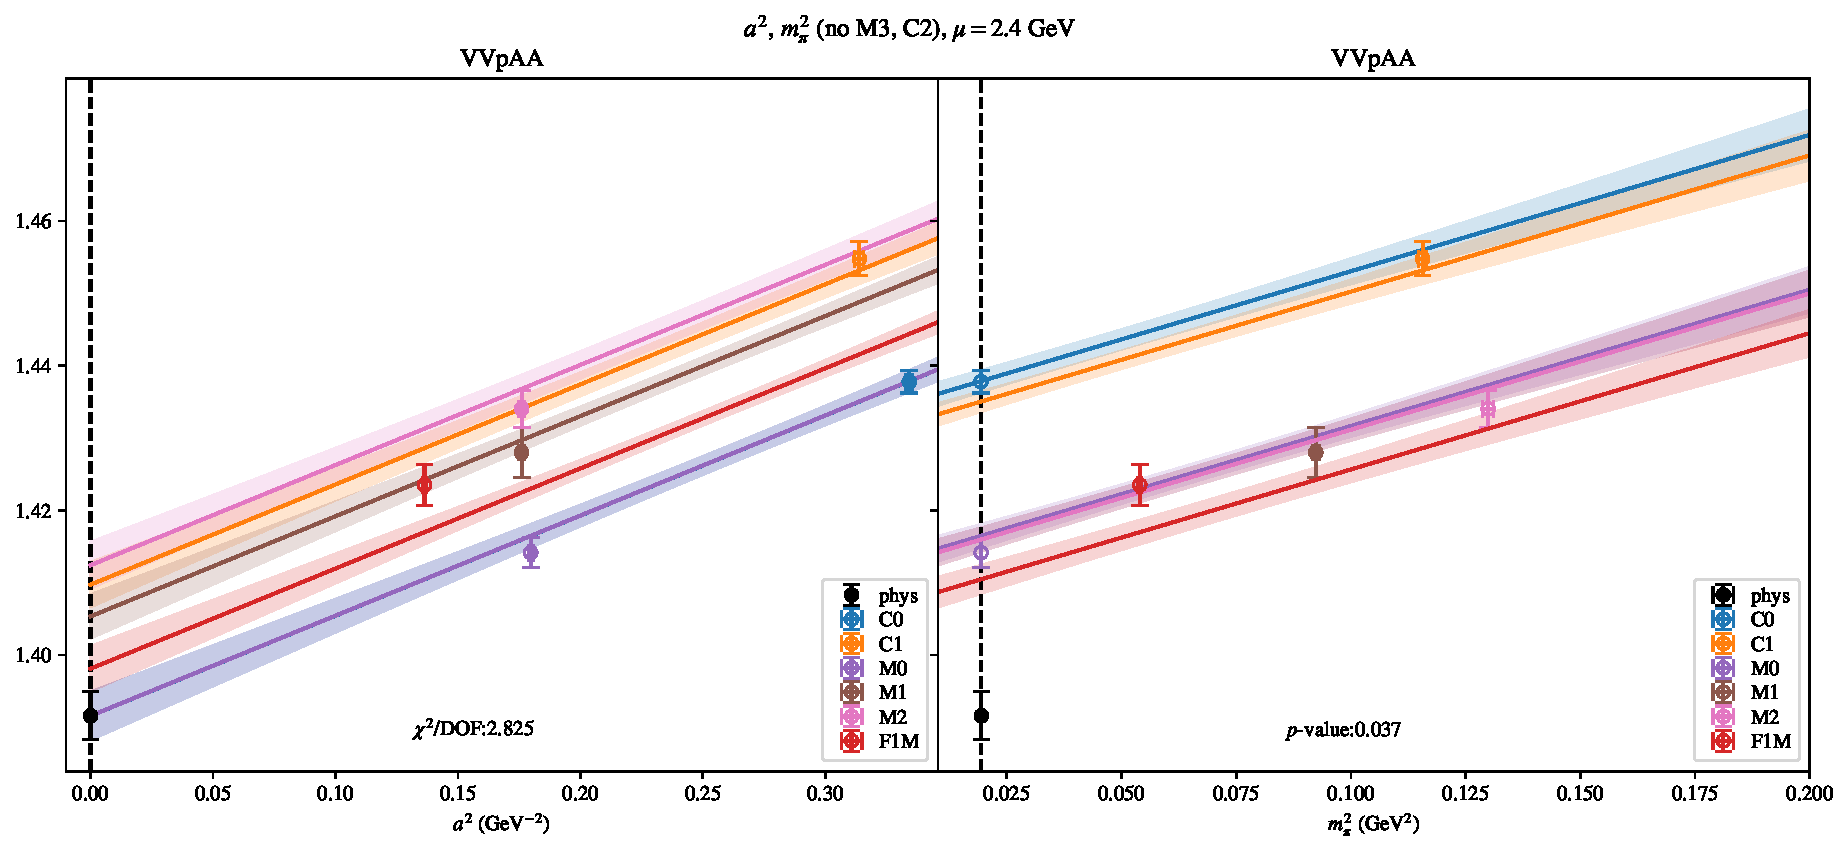
\includepdf[link, pages=-]{VVpAA/SUSY/bag_a2m2mcut_24.pdf}
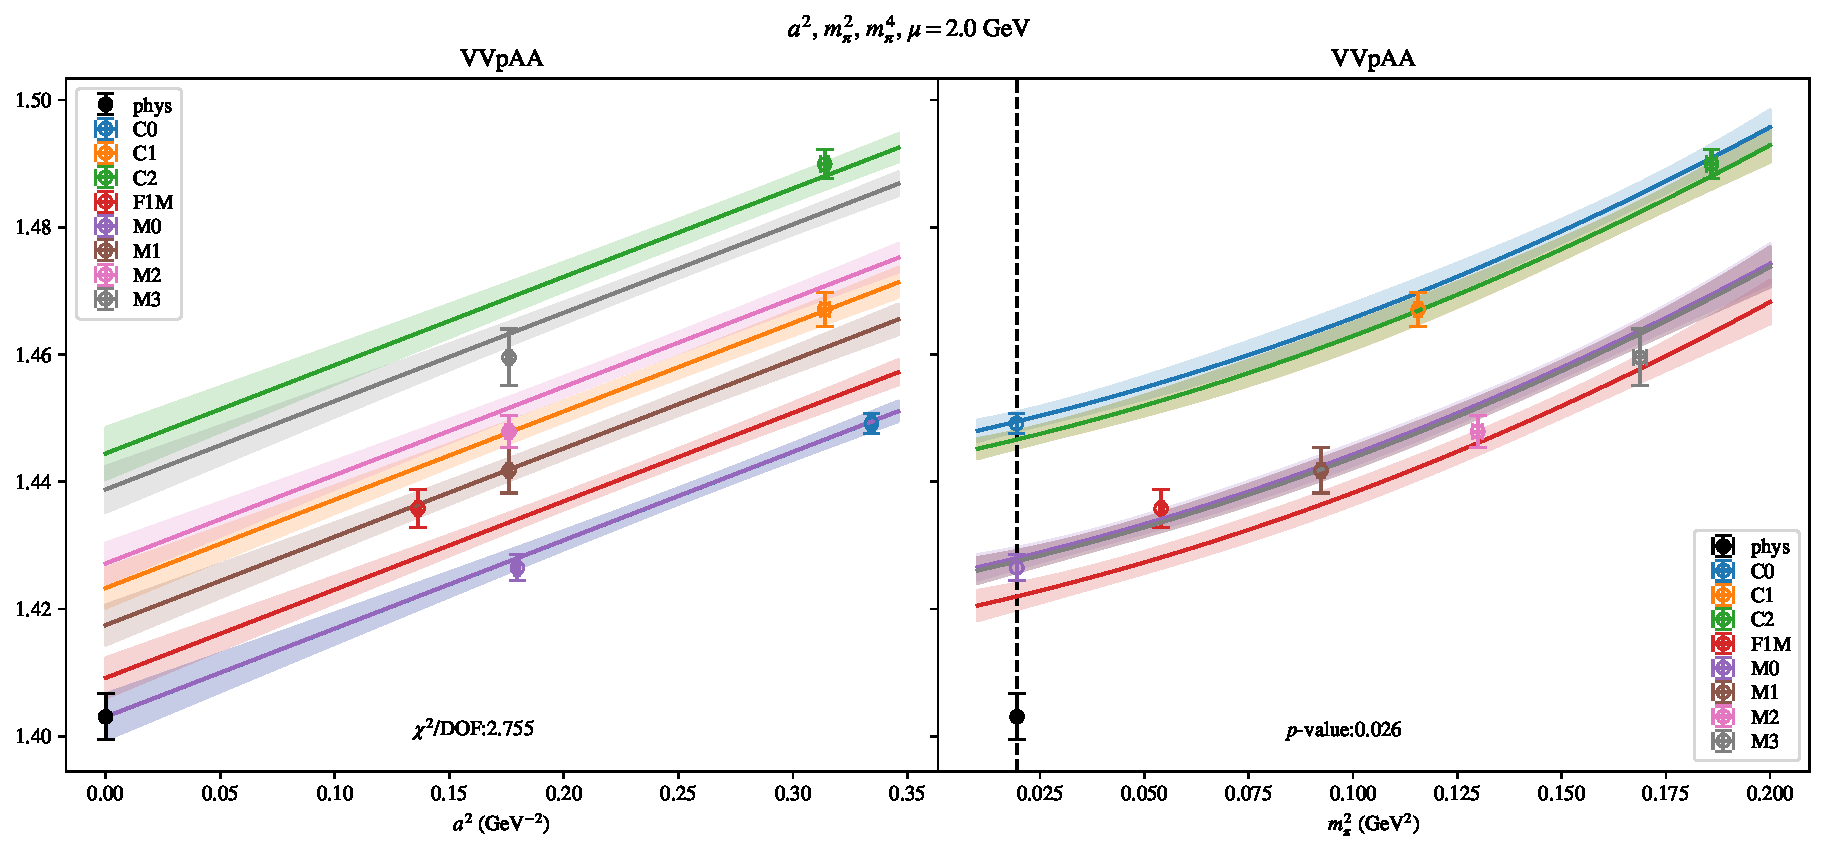
\includepdf[link, pages=-]{VVpAA/SUSY/bag_a2m2m4_20.pdf}
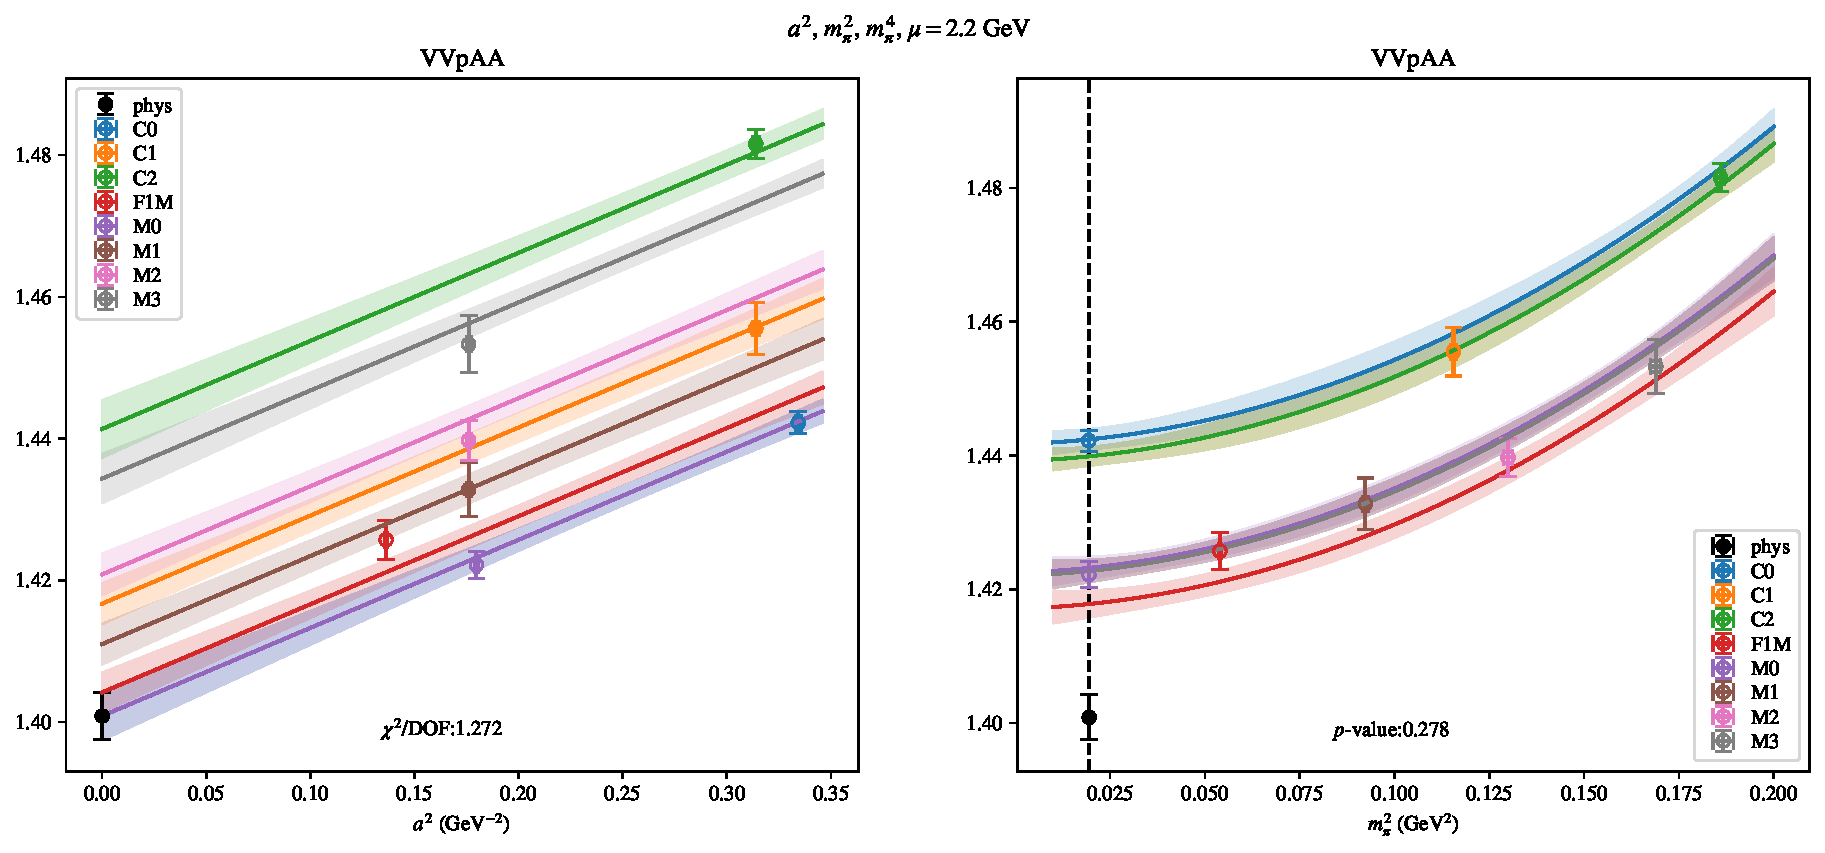
\includepdf[link, pages=-]{VVpAA/SUSY/bag_a2m2m4_22.pdf}
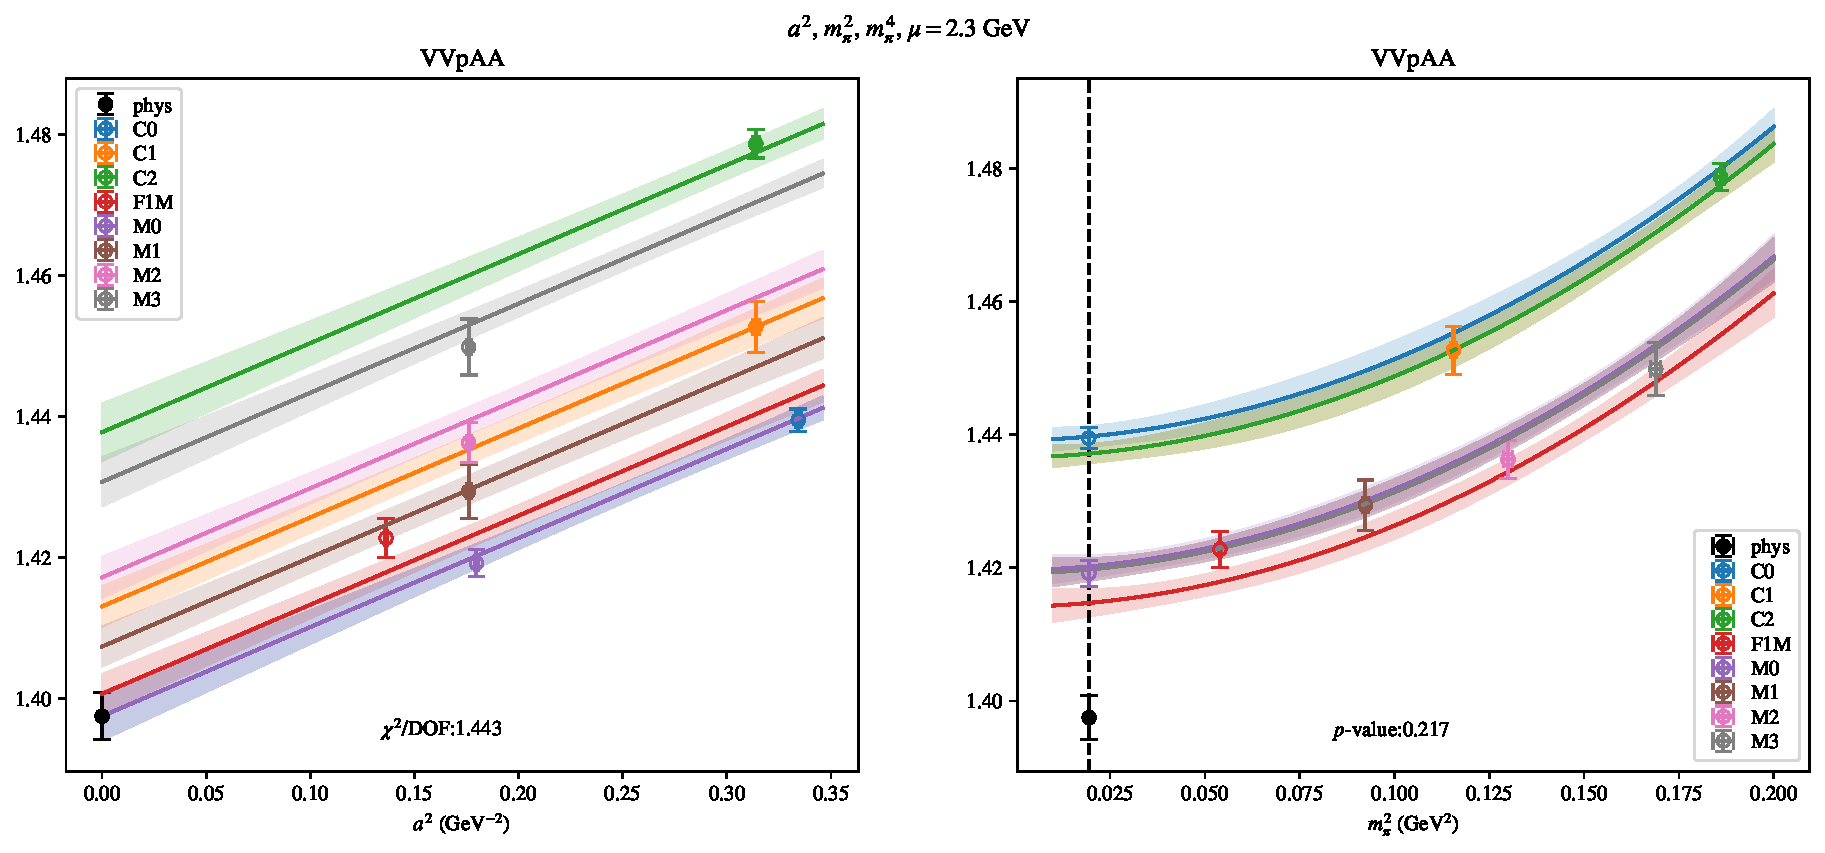
\includepdf[link, pages=-]{VVpAA/SUSY/bag_a2m2m4_23.pdf}
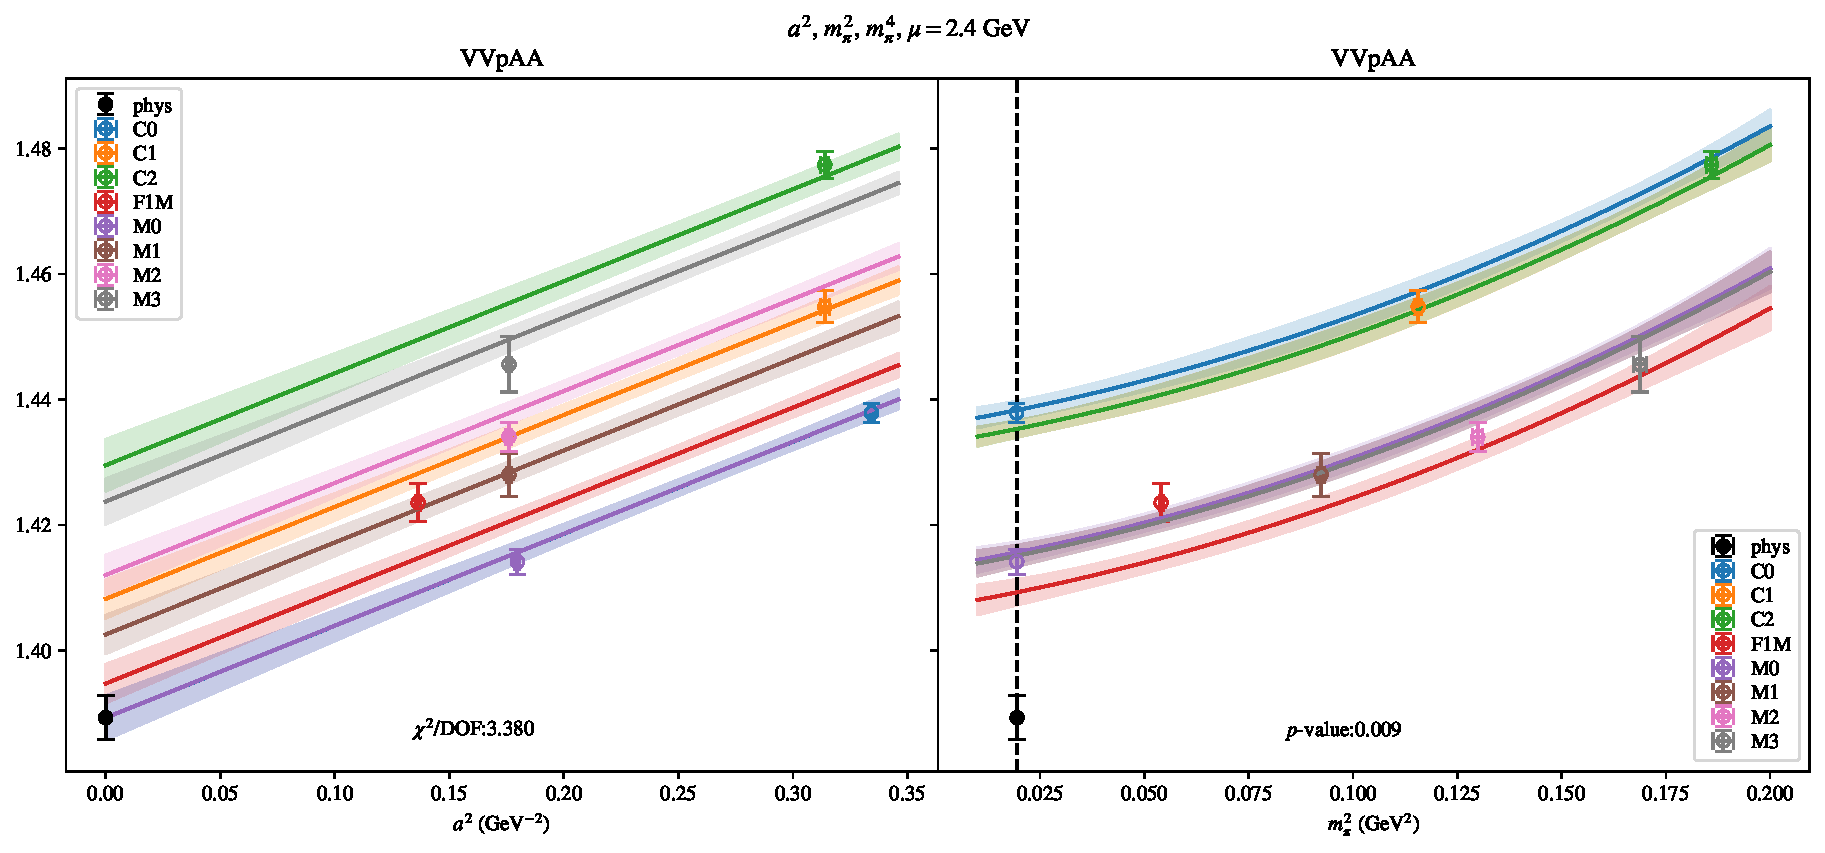
\includepdf[link, pages=-]{VVpAA/SUSY/bag_a2m2m4_24.pdf}
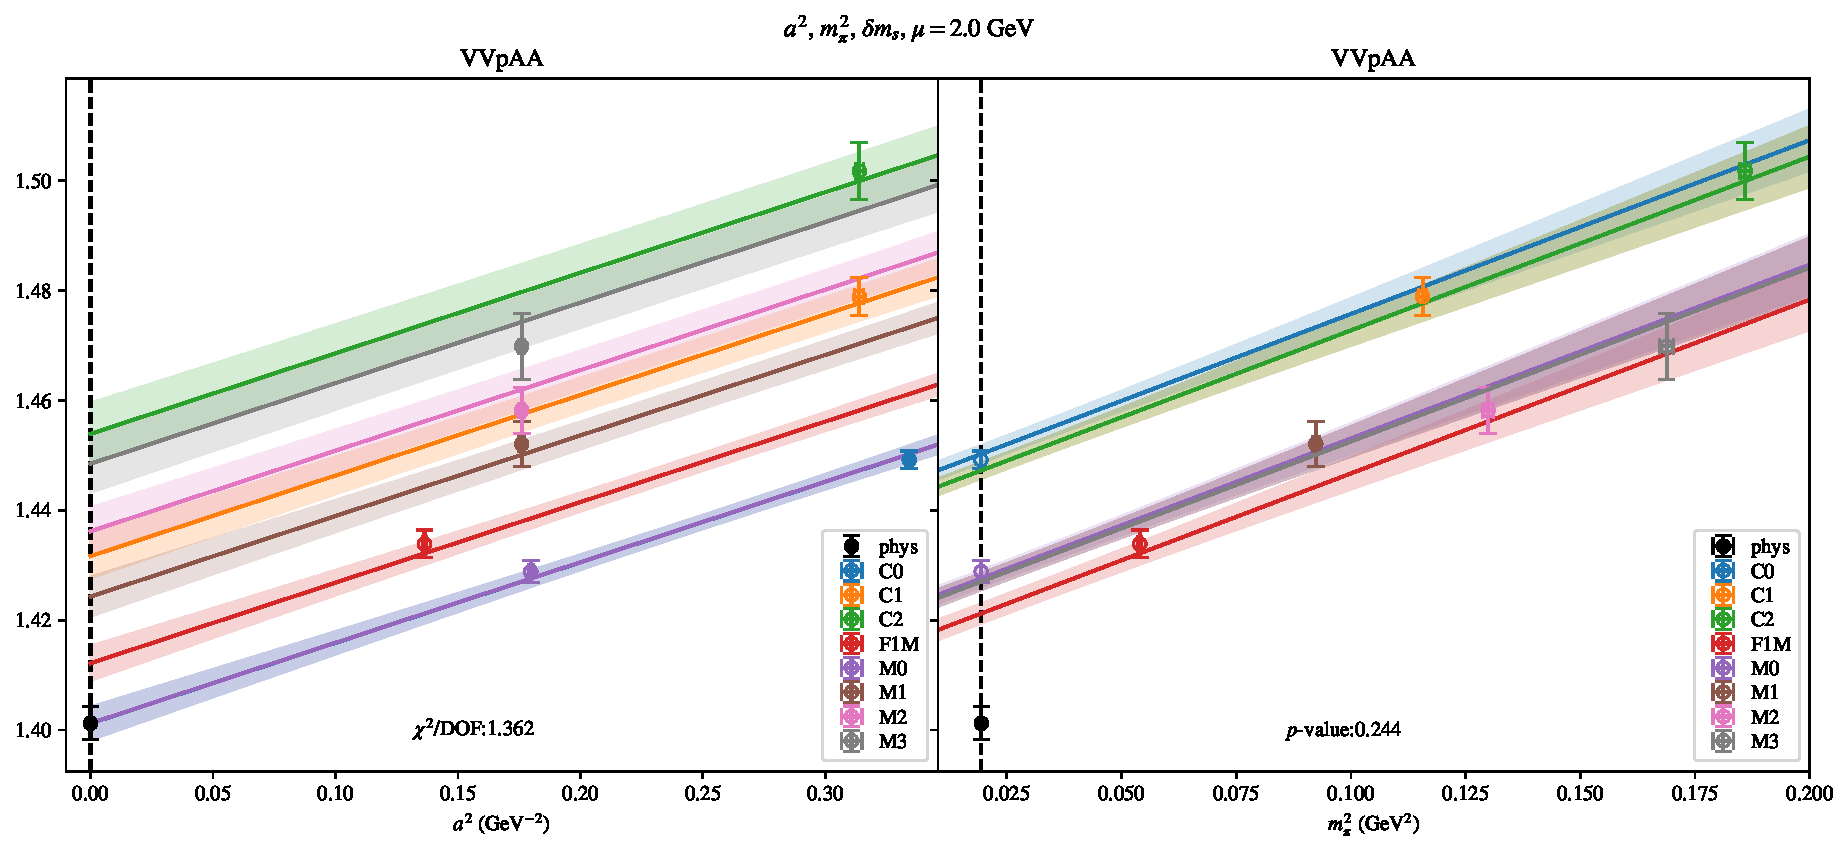
\includepdf[link, pages=-]{VVpAA/SUSY/bag_a2m2delm_20.pdf}
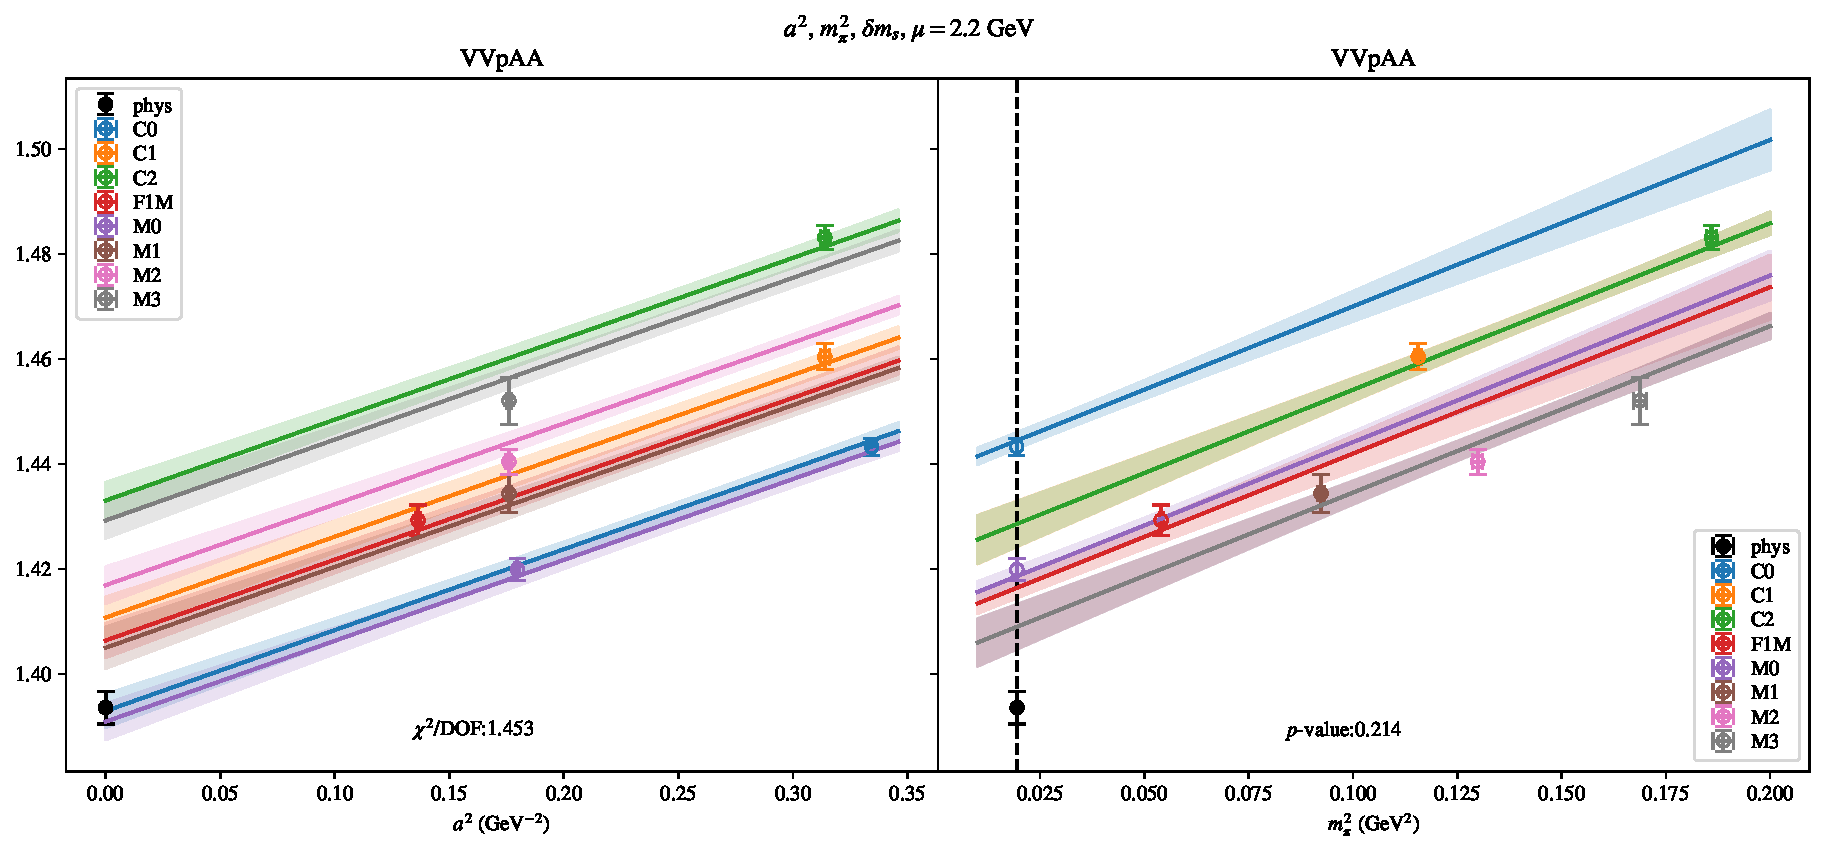
\includepdf[link, pages=-]{VVpAA/SUSY/bag_a2m2delm_22.pdf}
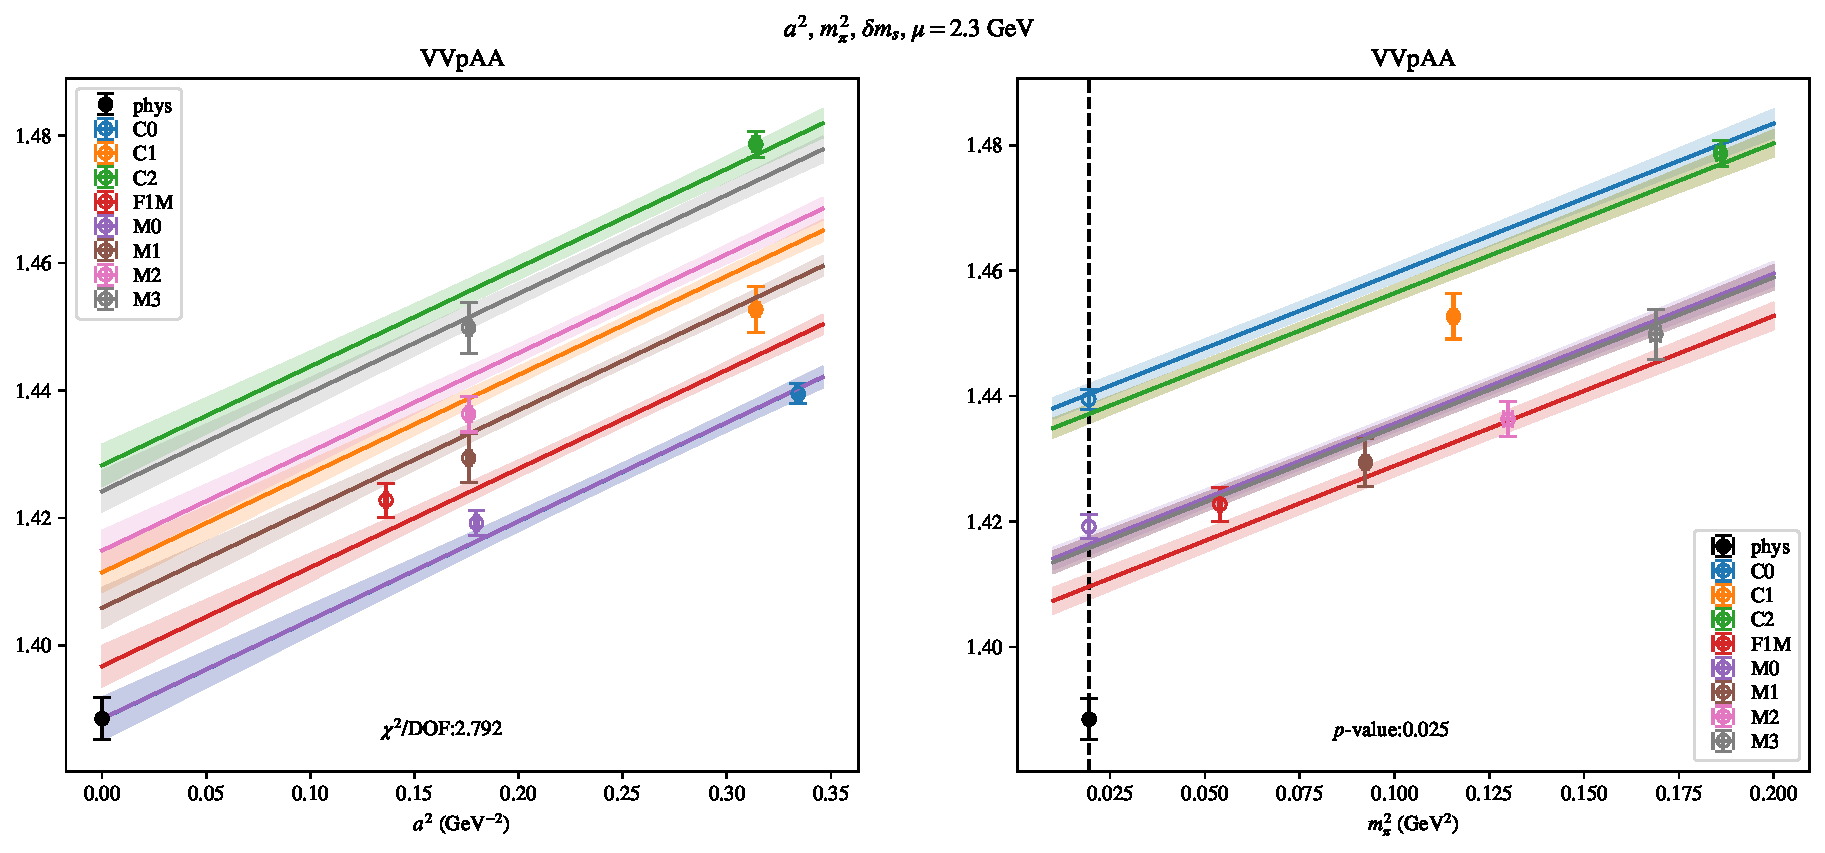
\includepdf[link, pages=-]{VVpAA/SUSY/bag_a2m2delm_23.pdf}
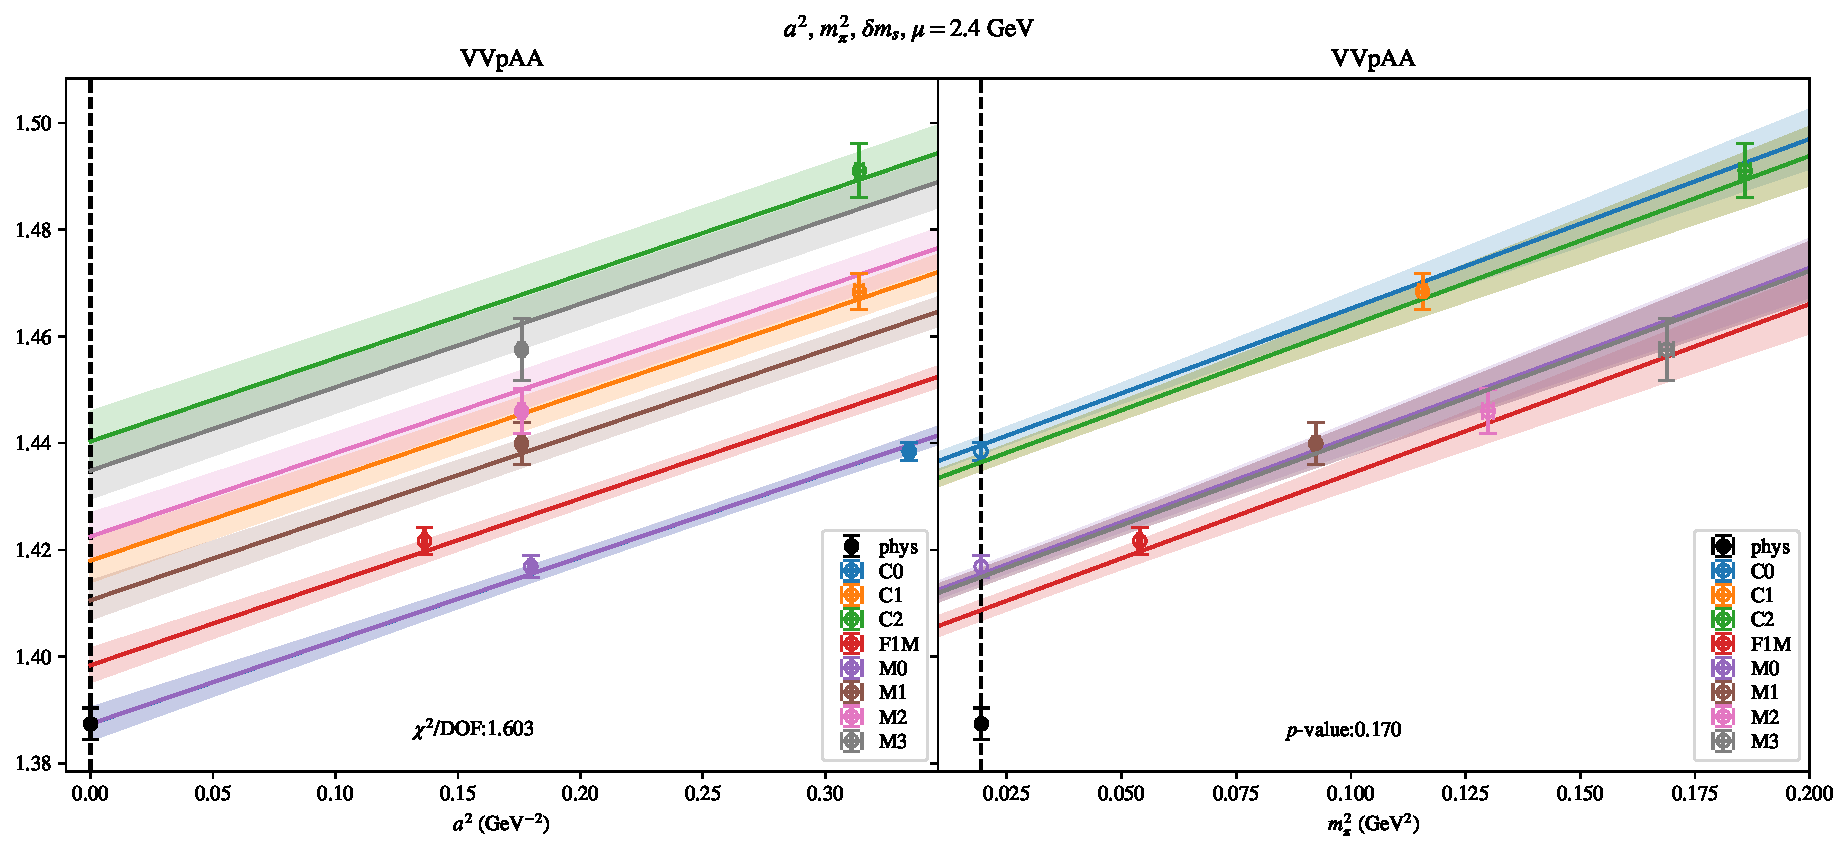
\includepdf[link, pages=-]{VVpAA/SUSY/bag_a2m2delm_24.pdf}
\clearpage
\section{$\mathcal{B}_2$}
\begin{table}[h!]
\begin{center}
\begin{tabular}{|c|c|c|c|c|c|c|}
\hline
$\mu$ (GeV) & $a^2$, $m_\pi^2$& $a^2$, $m_\pi^2$ (no C)& $a^2$, $m_\pi^2$, $a^4$& $a^2$, $m_\pi^2$ (no M3, C2)& $a^2$, $m_\pi^2$, $m_\pi^4$& $a^2$, $m_\pi^2$, $\delta m_s$\\
\hline
2.0& \hyperlink{VVmAA/SUSY/bag_a2m2_20.pdf.1}{\textbf{-0.9260(17)}: 3.665 (0.003)} & \hyperlink{VVmAA/SUSY/bag_a2m2noC_20.pdf.1}{\textbf{-0.9462(83)}: 2.165 (0.115)} & \hyperlink{VVmAA/SUSY/bag_a2a4m2_20.pdf.1}{\textbf{-0.948(13)}: 3.588 (0.006)} & \hyperlink{VVmAA/SUSY/bag_a2m2mcut_20.pdf.1}{\textbf{-0.9252(19)}: 3.556 (0.014)} & \hyperlink{VVmAA/SUSY/bag_a2m2m4_20.pdf.1}{\textbf{-0.9233(19)}: 2.331 (0.054)} & \hyperlink{VVmAA/SUSY/bag_a2m2delm_20.pdf.1}{\textbf{-0.9262(19)}: 4.626 (0.001)}\\
2.2& \hyperlink{VVmAA/SUSY/bag_a2m2_22.pdf.1}{\textbf{-0.9062(17)}: 4.709 (0.0)} & \hyperlink{VVmAA/SUSY/bag_a2m2noC_22.pdf.1}{\textbf{-0.9298(78)}: 1.765 (0.171)} & \hyperlink{VVmAA/SUSY/bag_a2a4m2_22.pdf.1}{\textbf{-0.929(13)}: 5.243 (0.0)} & \hyperlink{VVmAA/SUSY/bag_a2m2mcut_22.pdf.1}{\textbf{-0.9061(18)}: 4.644 (0.003)} & \hyperlink{VVmAA/SUSY/bag_a2m2m4_22.pdf.1}{\textbf{-0.9039(18)}: 3.852 (0.004)} & \hyperlink{VVmAA/SUSY/bag_a2m2delm_22.pdf.1}{\textbf{-0.9064(17)}: 5.734 (0.0)}\\
2.3& \hyperlink{VVmAA/SUSY/bag_a2m2_23.pdf.1}{\textbf{-0.8977(17)}: 5.386 (0.0)} & \hyperlink{VVmAA/SUSY/bag_a2m2noC_23.pdf.1}{\textbf{-0.9227(76)}: 1.916 (0.147)} & \hyperlink{VVmAA/SUSY/bag_a2a4m2_23.pdf.1}{\textbf{-0.923(13)}: 5.759 (0.0)} & \hyperlink{VVmAA/SUSY/bag_a2m2mcut_23.pdf.1}{\textbf{-0.8974(17)}: 6.304 (0.0)} & \hyperlink{VVmAA/SUSY/bag_a2m2m4_23.pdf.1}{\textbf{-0.8949(17)}: 4.488 (0.001)} & \hyperlink{VVmAA/SUSY/bag_a2m2delm_23.pdf.1}{\textbf{-0.8975(17)}: 6.701 (0.0)}\\
2.4& \hyperlink{VVmAA/SUSY/bag_a2m2_24.pdf.1}{\textbf{-0.8897(17)}: 5.736 (0.0)} & \hyperlink{VVmAA/SUSY/bag_a2m2noC_24.pdf.1}{\textbf{-0.9155(76)}: 1.907 (0.148)} & \hyperlink{VVmAA/SUSY/bag_a2a4m2_24.pdf.1}{\textbf{-0.916(13)}: 6.047 (0.0)} & \hyperlink{VVmAA/SUSY/bag_a2m2mcut_24.pdf.1}{\textbf{-0.8897(16)}: 7.106 (0.0)} & \hyperlink{VVmAA/SUSY/bag_a2m2m4_24.pdf.1}{\textbf{-0.8873(18)}: 4.833 (0.001)} & \hyperlink{VVmAA/SUSY/bag_a2m2delm_24.pdf.1}{\textbf{-0.8897(16)}: 7.381 (0.0)}\\
\hline
\end{tabular}
\caption{Physical point value from chiral and continuum extrapolation at renormalisation scale $\mu$. Entries are \textbf{value(error)}: $\chi^2/\text{DOF}$ ($p$-value).}
\end{center}
\end{table}
\begin{table}[h!]
\begin{center}
\begin{tabular}{|c c|c|c|c|c|c|c|}
\hline
$\mu$ (GeV) &  & $a^2$, $m_\pi^2$& $a^2$, $m_\pi^2$ (no C)& $a^2$, $m_\pi^2$, $a^4$& $a^2$, $m_\pi^2$ (no M3, C2)& $a^2$, $m_\pi^2$, $m_\pi^4$& $a^2$, $m_\pi^2$, $\delta m_s$\\
\hline
\multirow{3}{0.5in}{2.0} & $\alpha$ & -0.3487(66)& -0.232(48)& -0.15(12)& -0.3503(74)& -0.3568(70)& -0.3481(73)\\
 & $\beta$ & -0.00626(15)& -0.00587(29)& -0.00635(15)& -0.00672(27)& -0.00871(82)& -0.00624(35)\\
 & $\gamma$ &  &  & -0.40(25)&  & 0.000223(72)& 0.0001(138)\\
\hline
\multirow{3}{0.5in}{2.2} & $\alpha$ & -0.3834(66)& -0.249(46)& -0.17(12)& -0.3827(69)& -0.3905(66)& -0.3830(71)\\
 & $\beta$ & -0.00649(14)& -0.00597(25)& -0.00660(14)& -0.00695(26)& -0.00863(72)& -0.00657(36)\\
 & $\gamma$ &  &  & -0.43(24)&  & 0.000193(64)& 0.002(14)\\
\hline
\multirow{3}{0.5in}{2.3} & $\alpha$ & -0.3986(64)& -0.256(44)& -0.17(12)& -0.3985(64)& -0.4071(66)& -0.3993(70)\\
 & $\beta$ & -0.00652(14)& -0.00599(24)& -0.00661(14)& -0.00692(24)& -0.00873(70)& -0.00653(33)\\
 & $\gamma$ &  &  & -0.47(25)&  & 0.000201(62)& 0.0006(139)\\
\hline
\multirow{3}{0.5in}{2.4} & $\alpha$ & -0.4131(65)& -0.267(44)& -0.18(12)& -0.4122(63)& -0.4205(66)& -0.4133(67)\\
 & $\beta$ & -0.00654(14)& -0.00600(24)& -0.00666(14)& -0.00691(24)& -0.00873(71)& -0.00662(34)\\
 & $\gamma$ &  &  & -0.48(24)&  & 0.000199(63)& 0.003(14)\\
\hline
\end{tabular}
\caption{Fit values of coefficients in $Q = Q_{phys} + \mathbf{\alpha} a^2 + \mathbf{\beta}\left(\frac{m_\pi^2}{f_\pi^2}-\frac{m_{\pi,PDG}^2}{f_\pi^2}\right) + \gamma(\ldots)$}
\end{center}
\end{table}
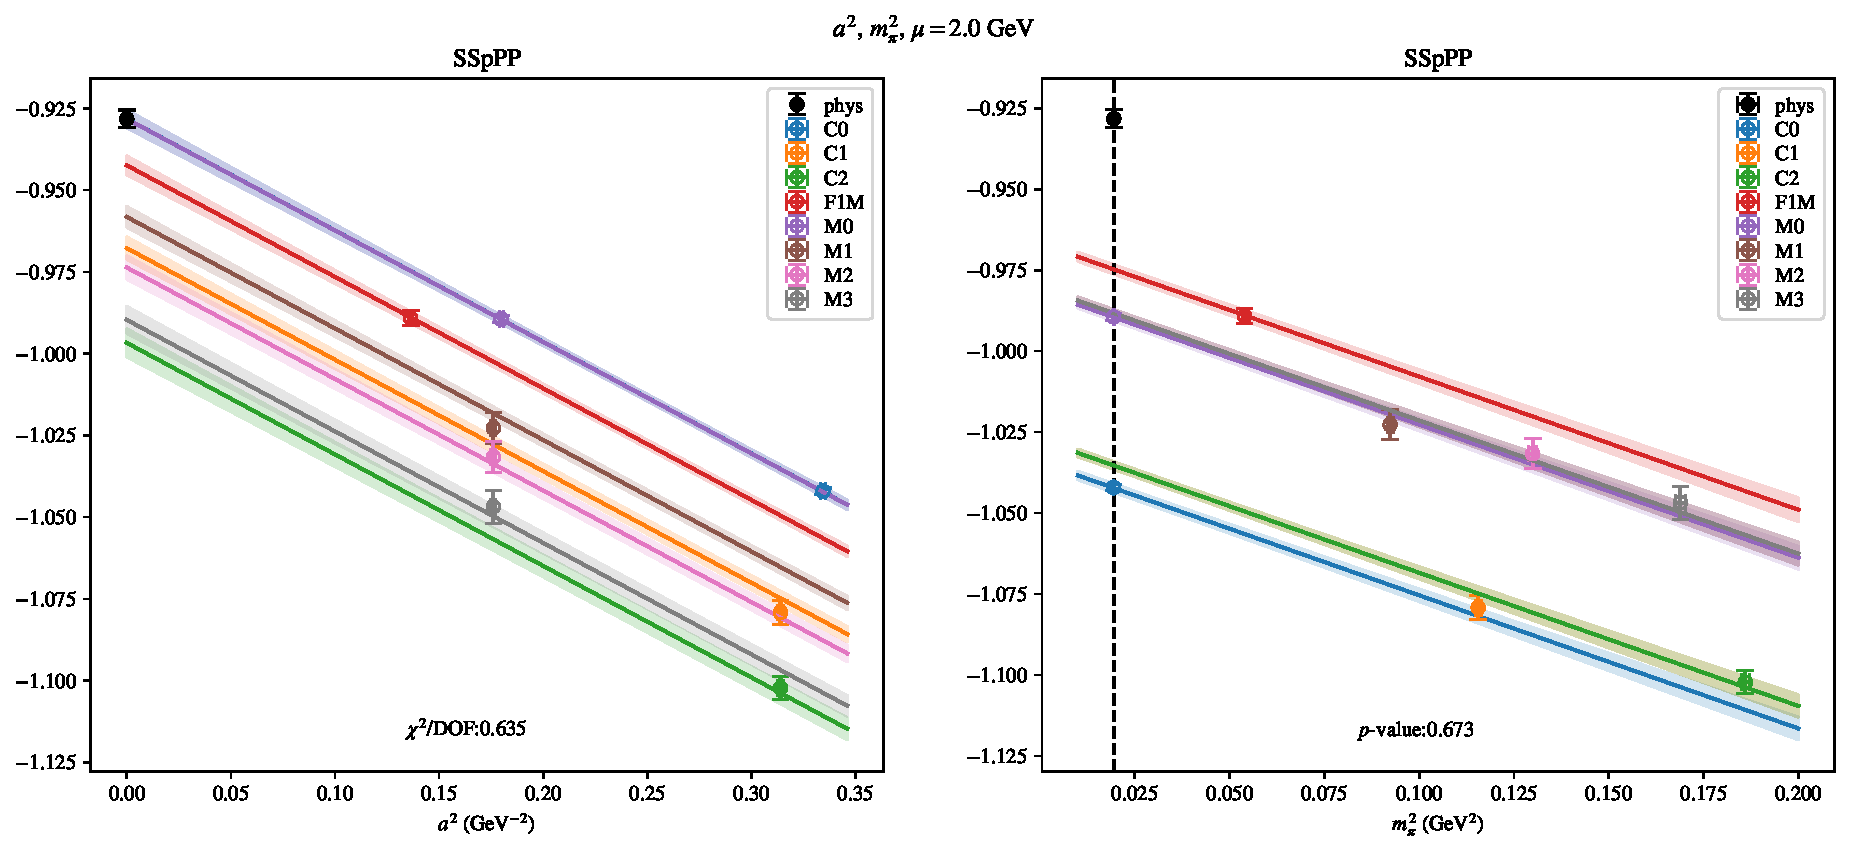
\includepdf[link, pages=-]{VVmAA/SUSY/bag_a2m2_20.pdf}
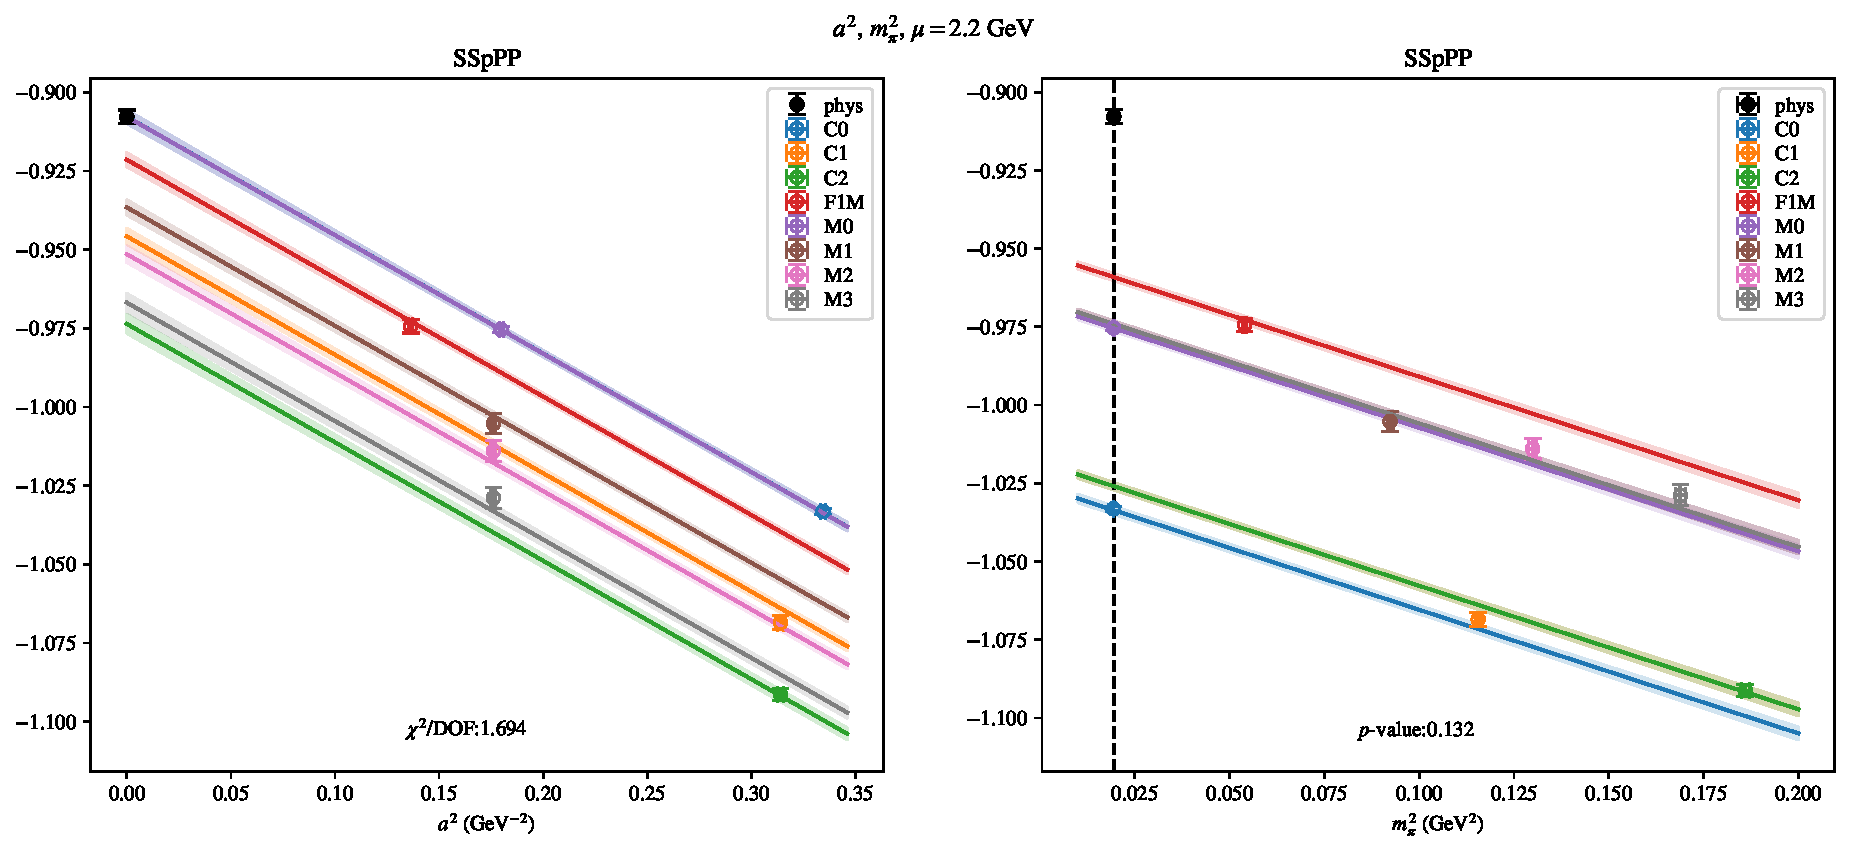
\includepdf[link, pages=-]{VVmAA/SUSY/bag_a2m2_22.pdf}
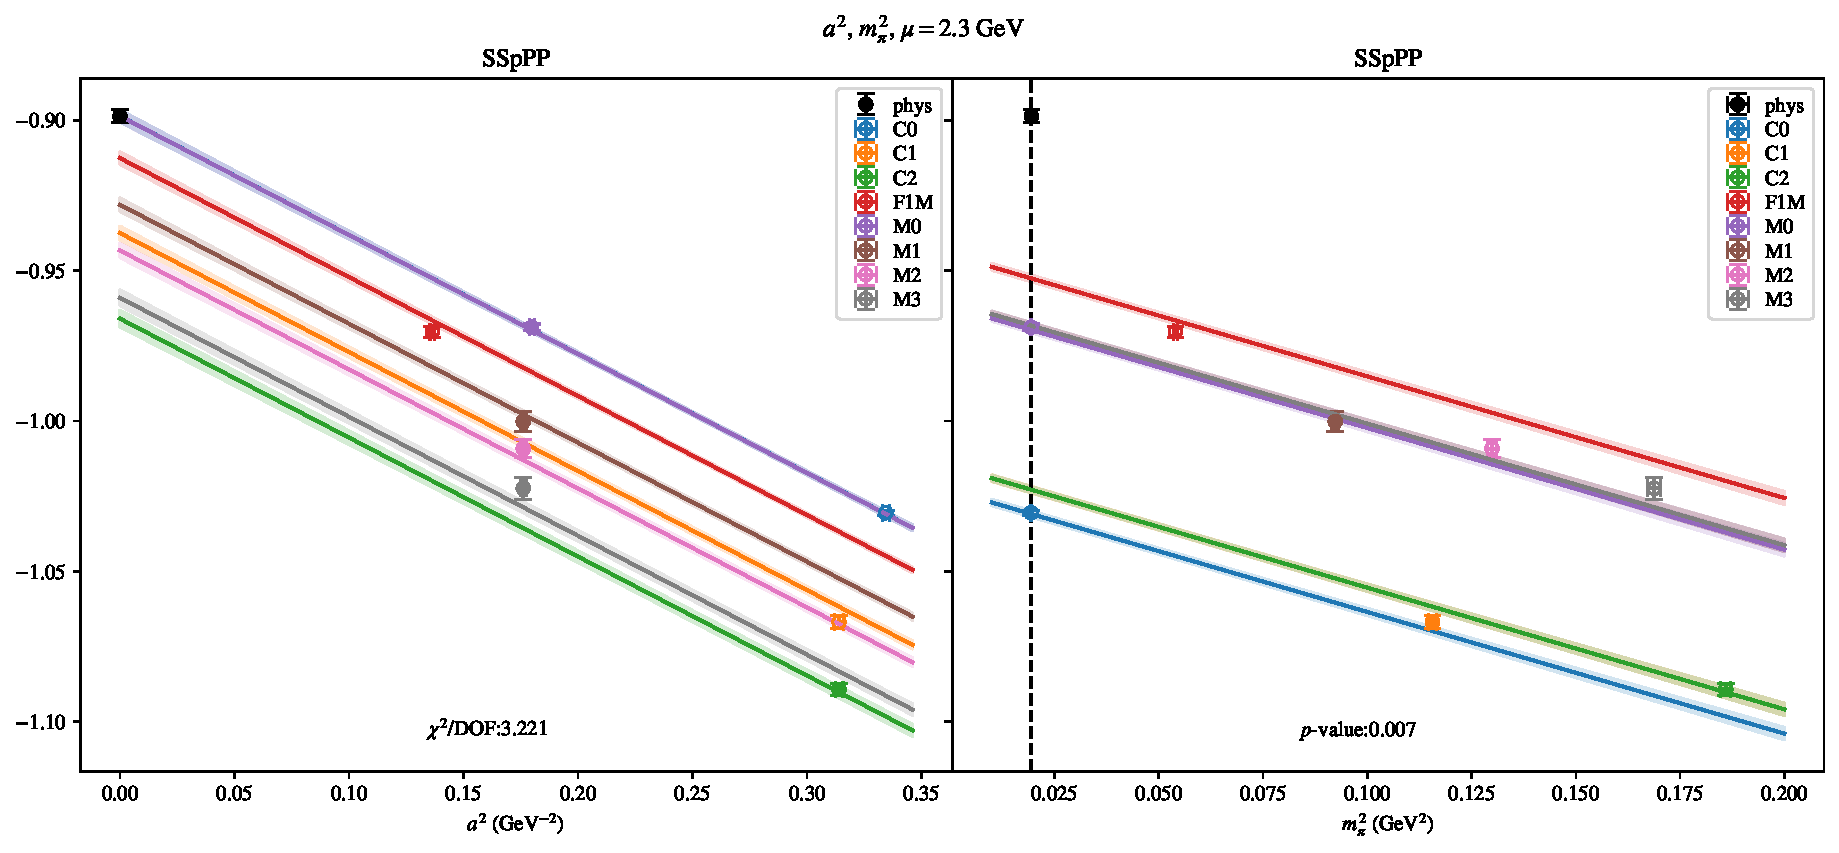
\includepdf[link, pages=-]{VVmAA/SUSY/bag_a2m2_23.pdf}
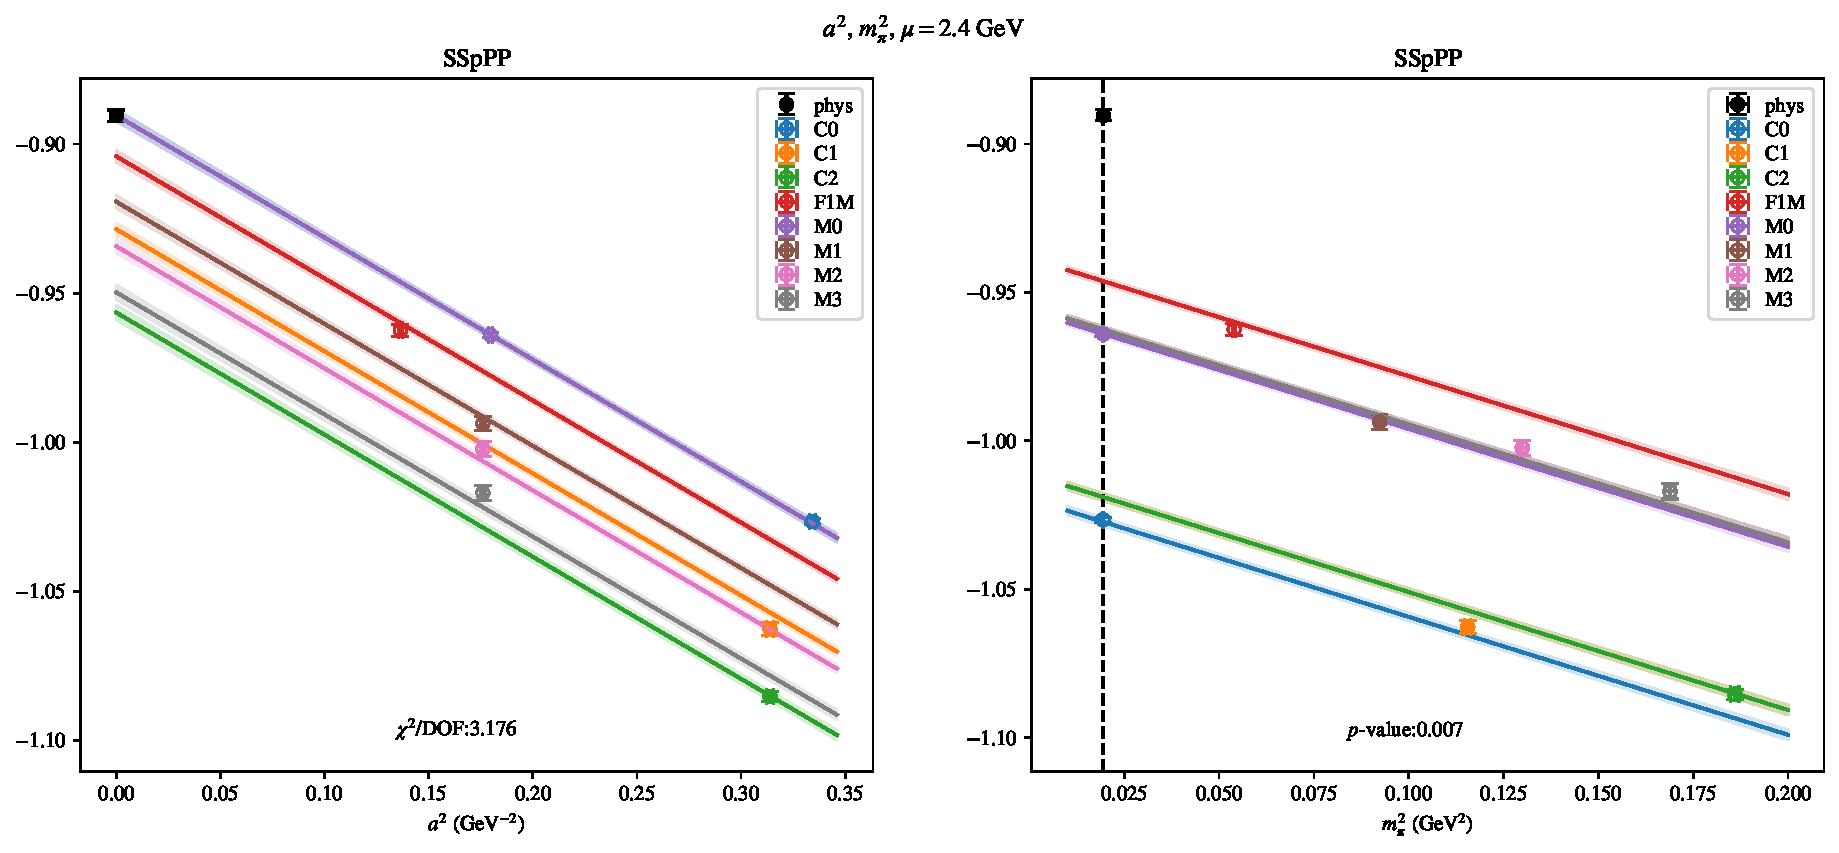
\includepdf[link, pages=-]{VVmAA/SUSY/bag_a2m2_24.pdf}
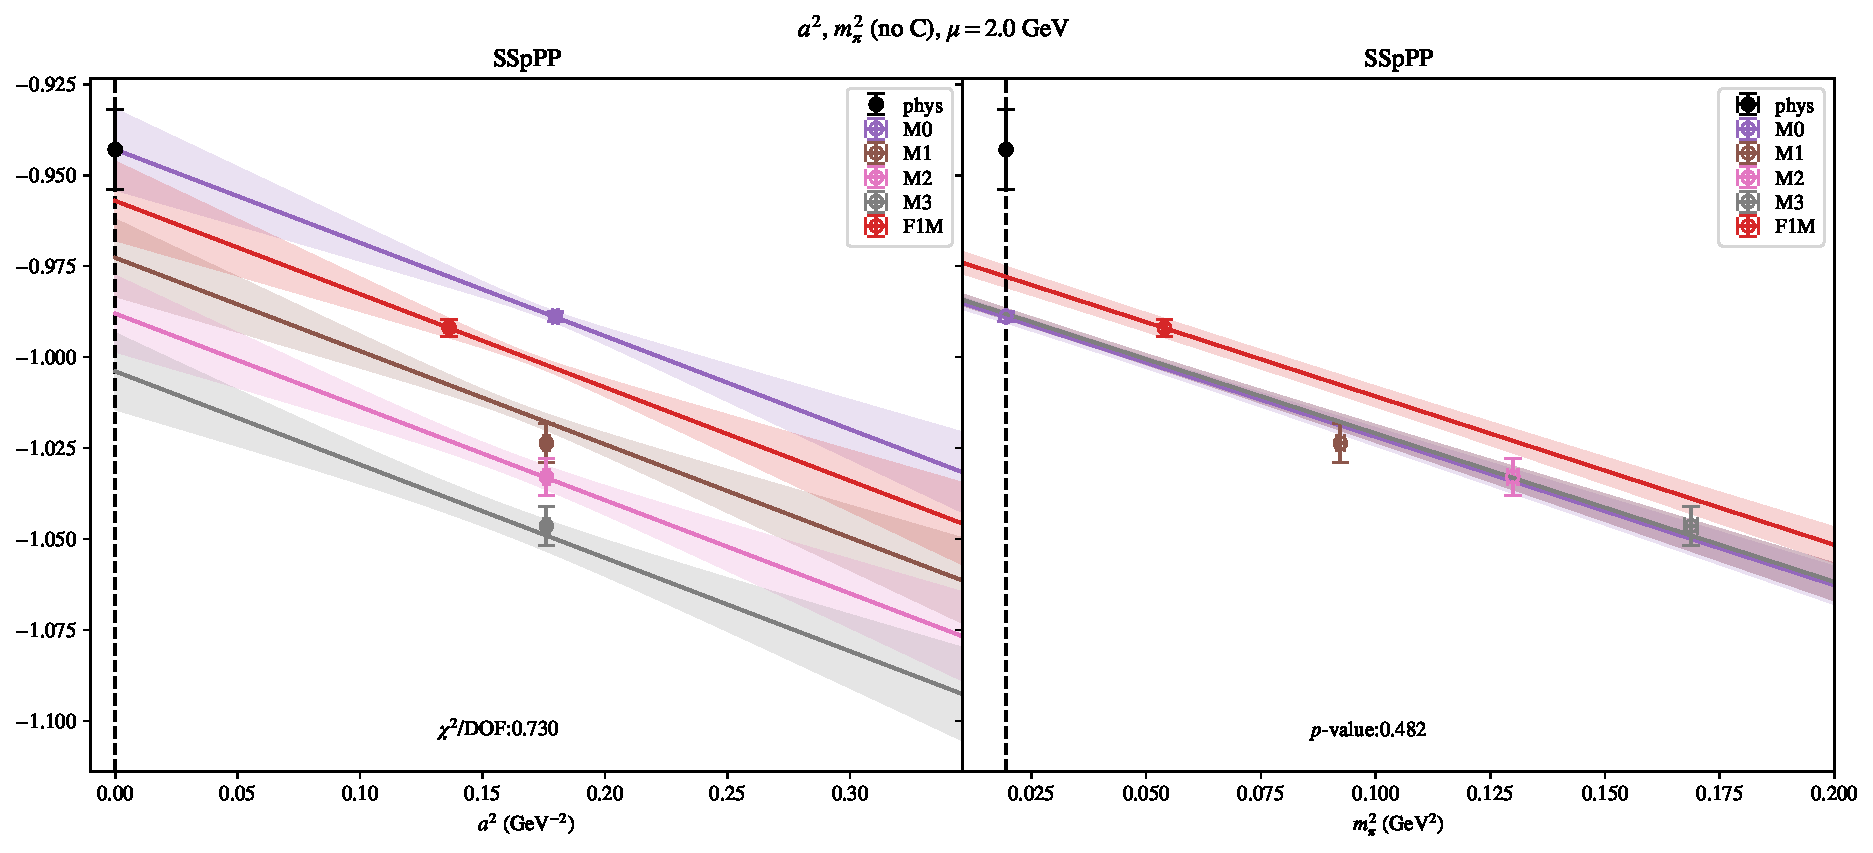
\includepdf[link, pages=-]{VVmAA/SUSY/bag_a2m2noC_20.pdf}
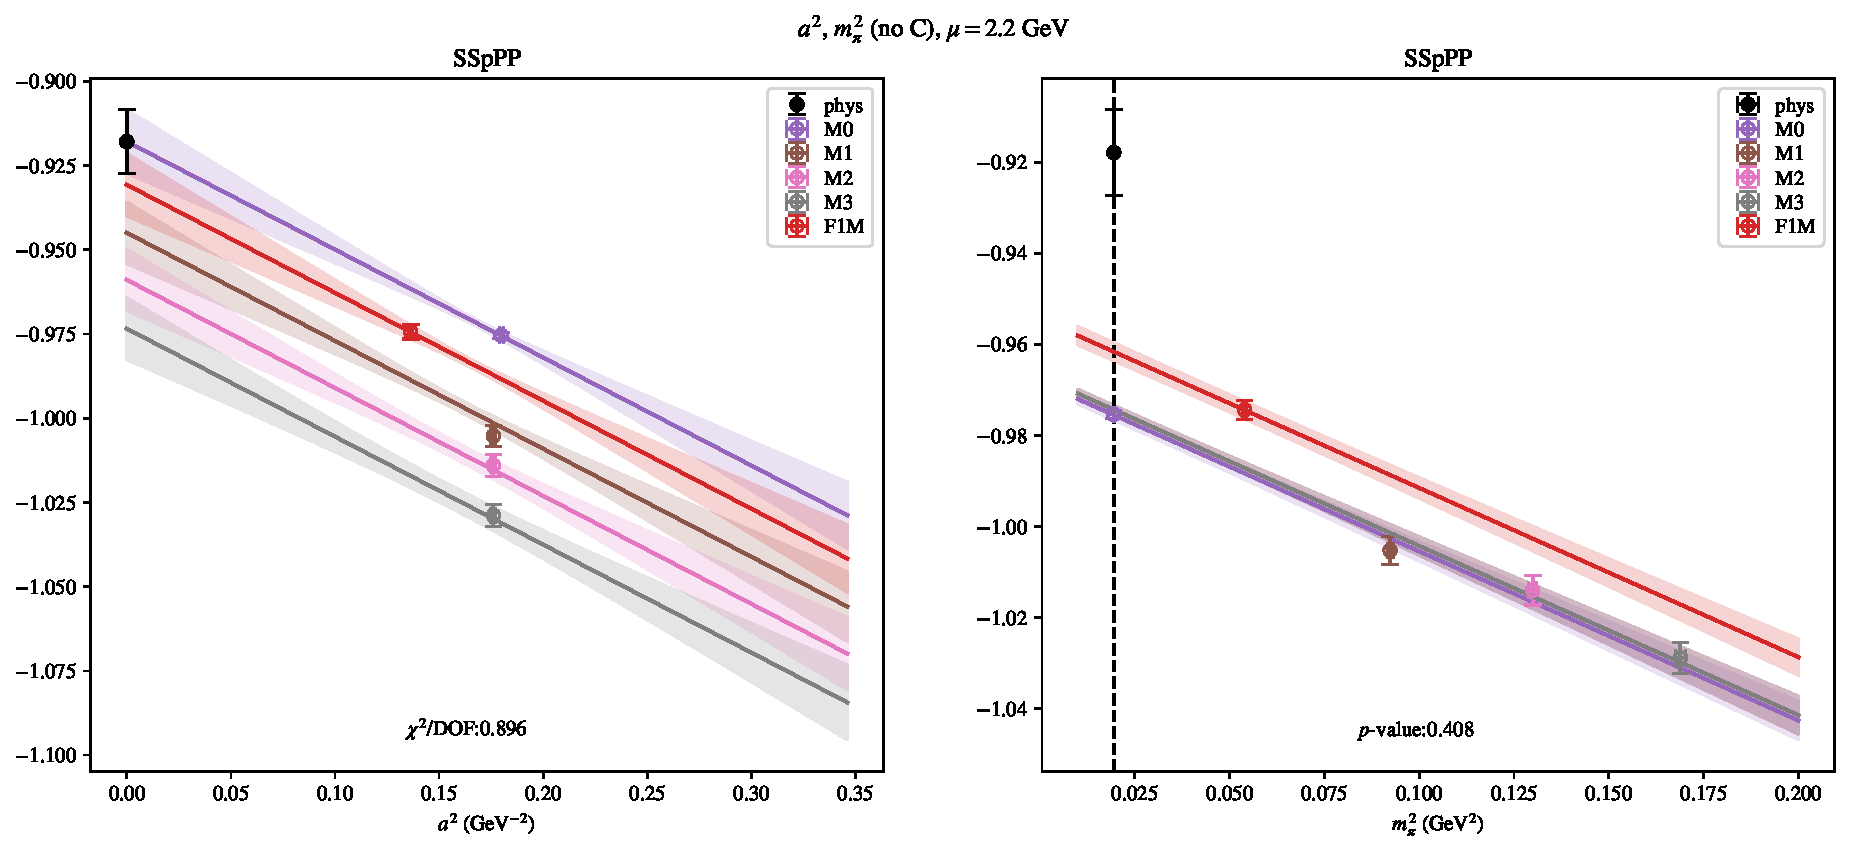
\includepdf[link, pages=-]{VVmAA/SUSY/bag_a2m2noC_22.pdf}
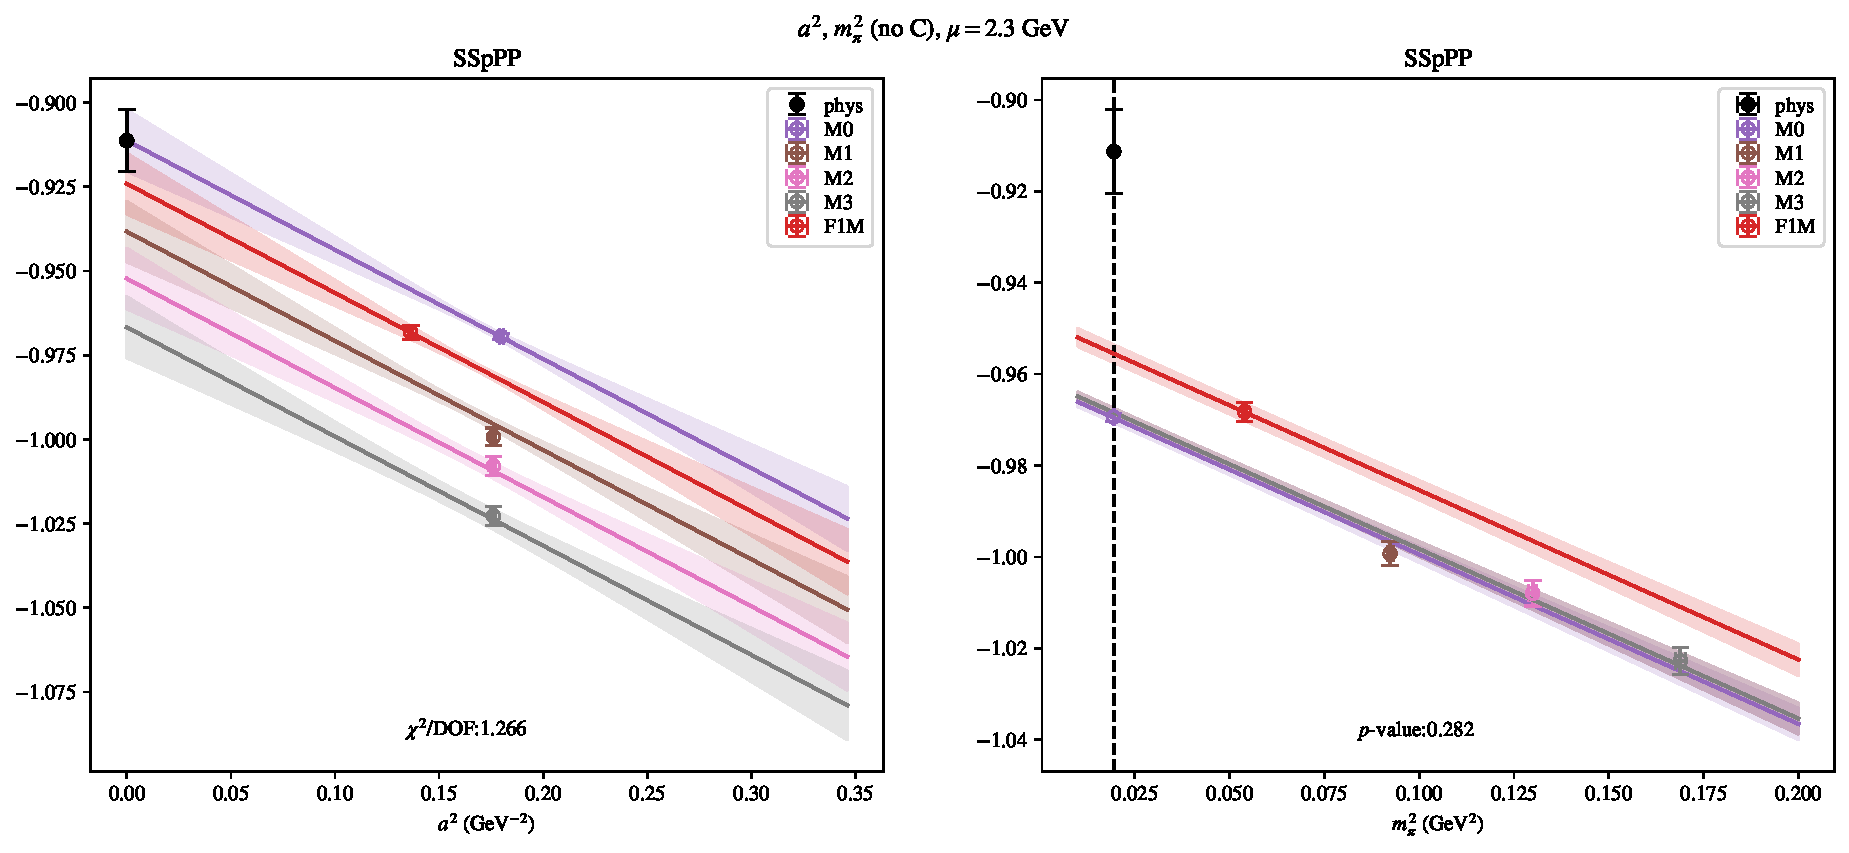
\includepdf[link, pages=-]{VVmAA/SUSY/bag_a2m2noC_23.pdf}
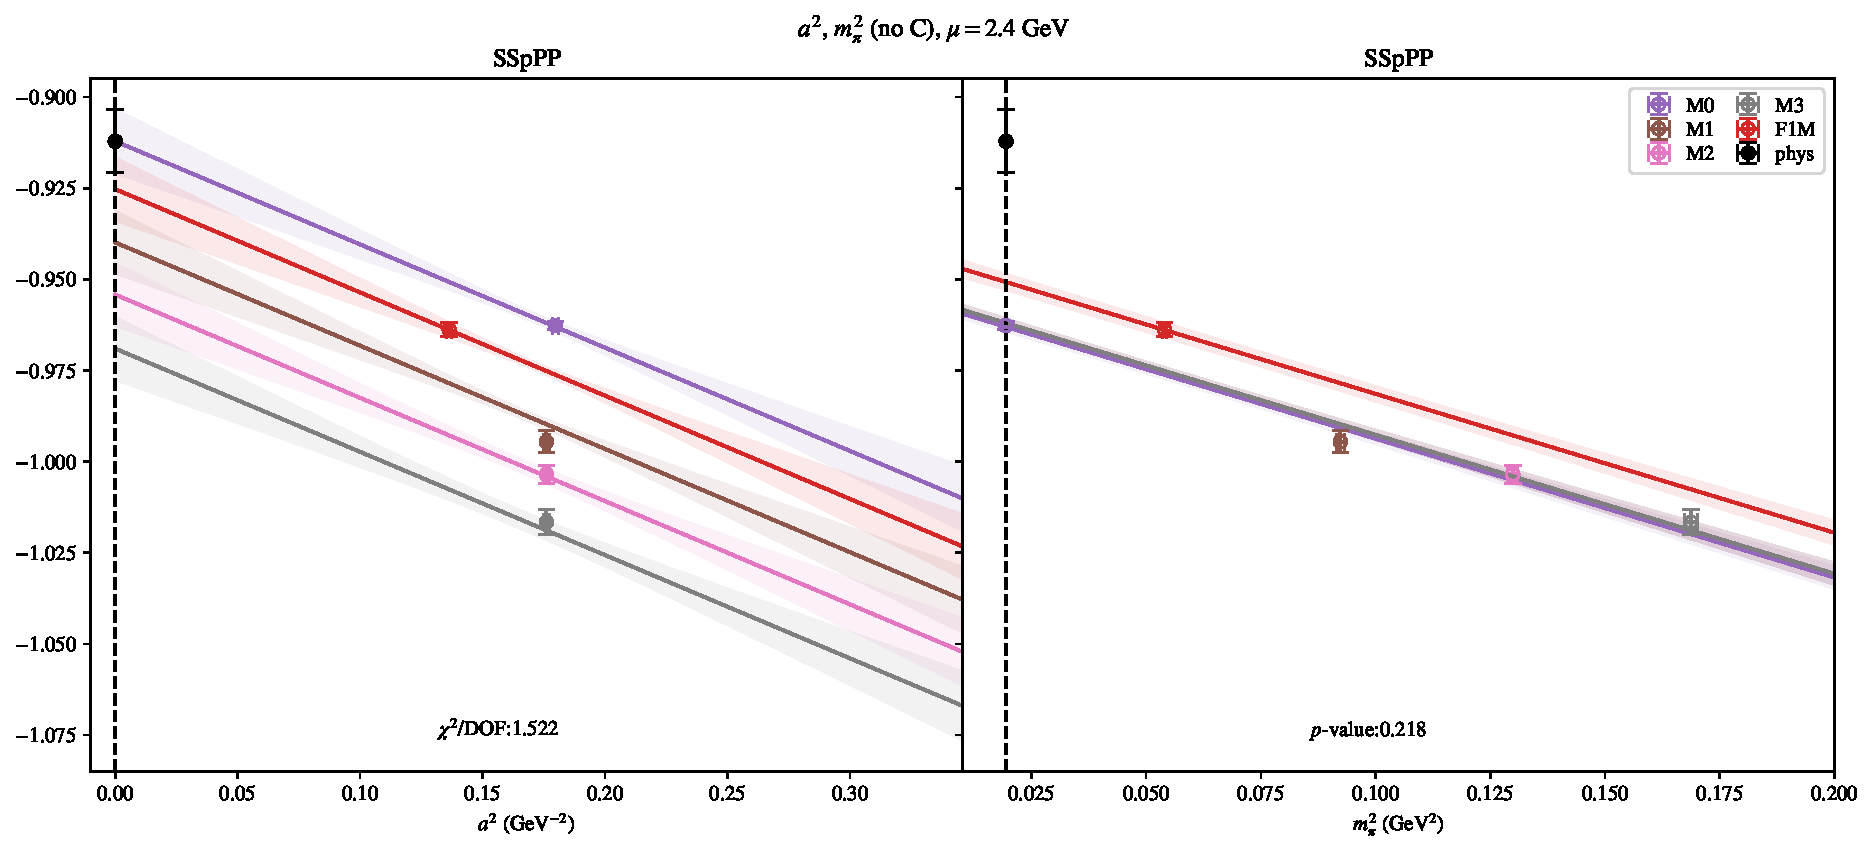
\includepdf[link, pages=-]{VVmAA/SUSY/bag_a2m2noC_24.pdf}
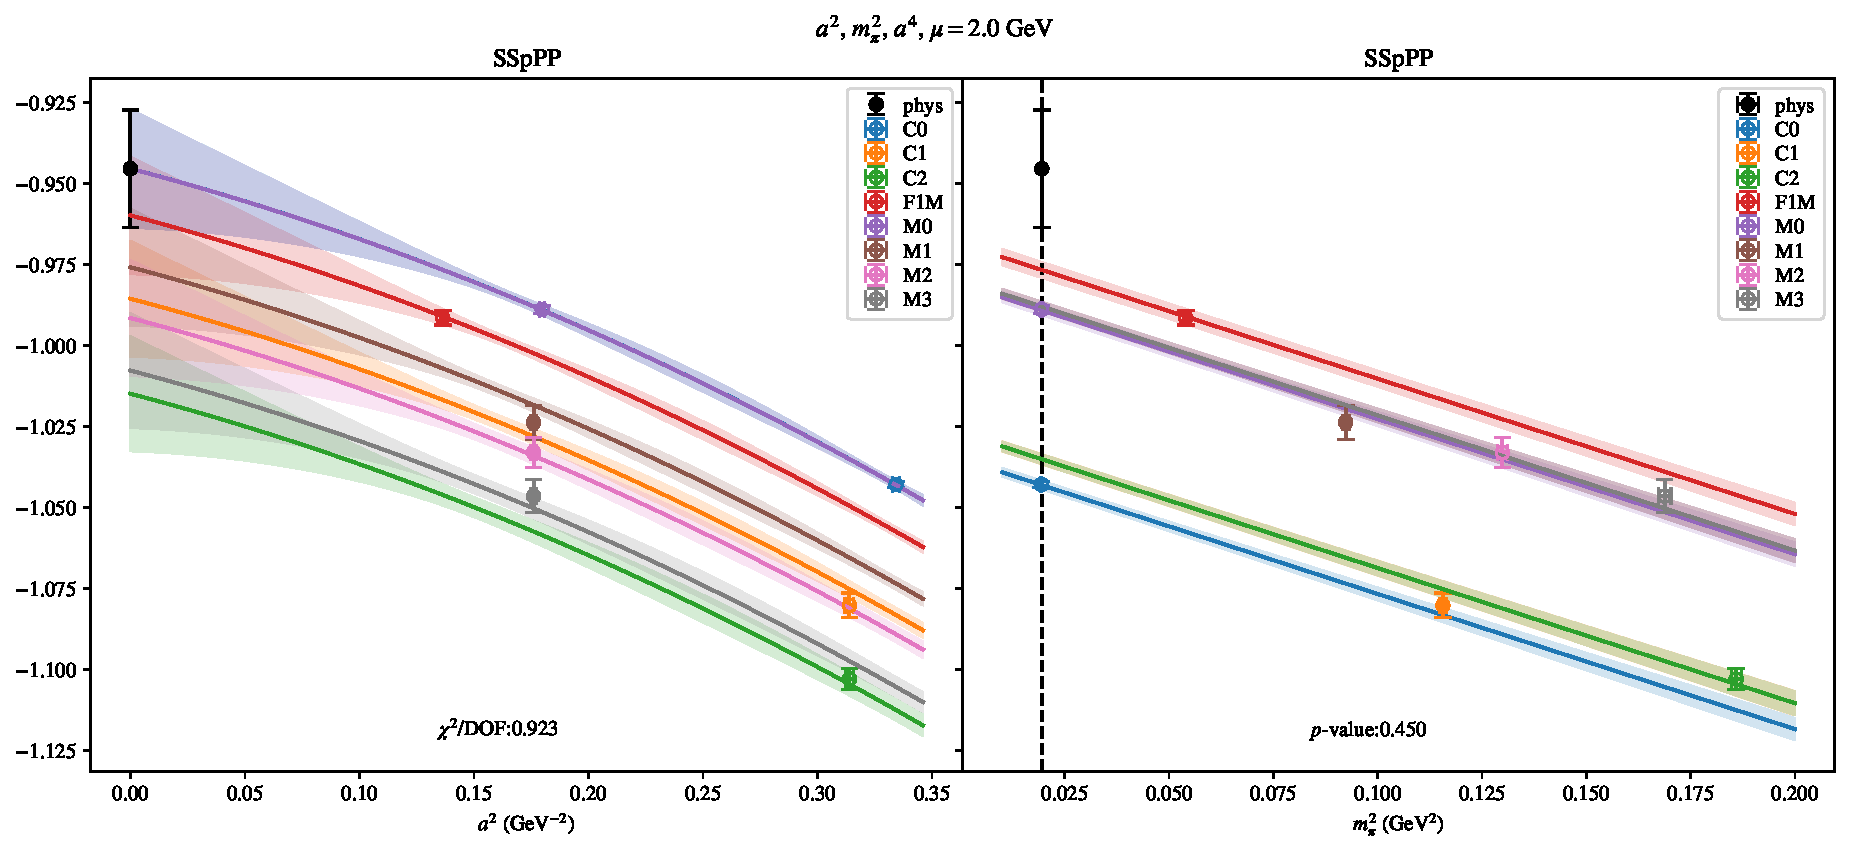
\includepdf[link, pages=-]{VVmAA/SUSY/bag_a2a4m2_20.pdf}
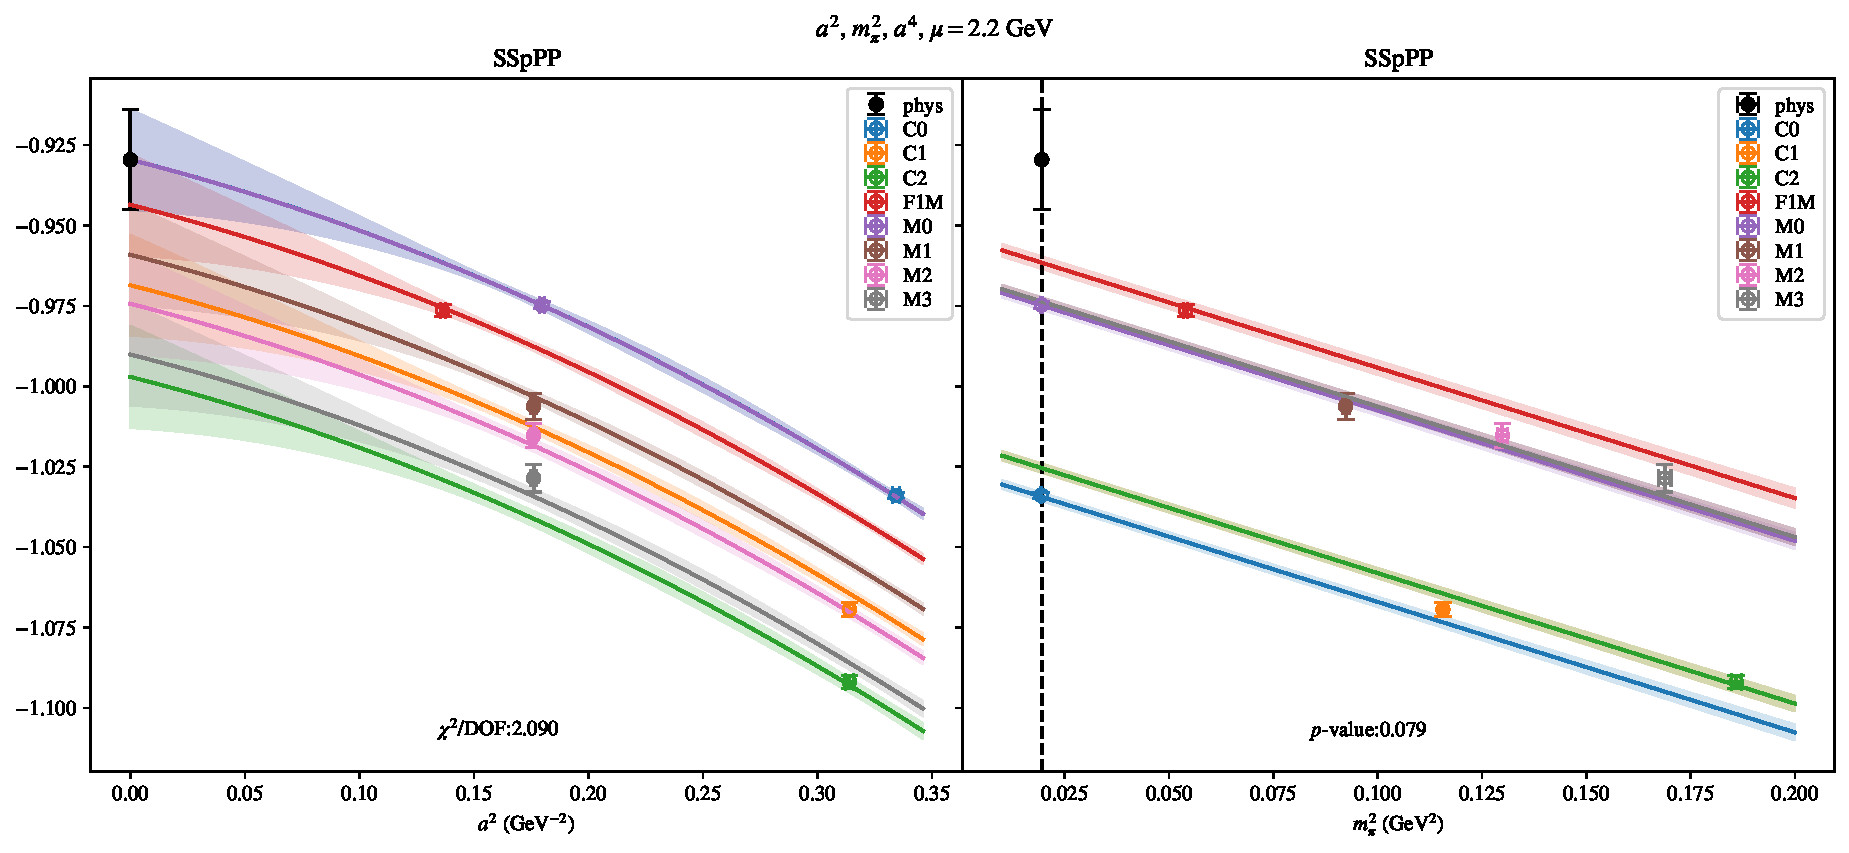
\includepdf[link, pages=-]{VVmAA/SUSY/bag_a2a4m2_22.pdf}
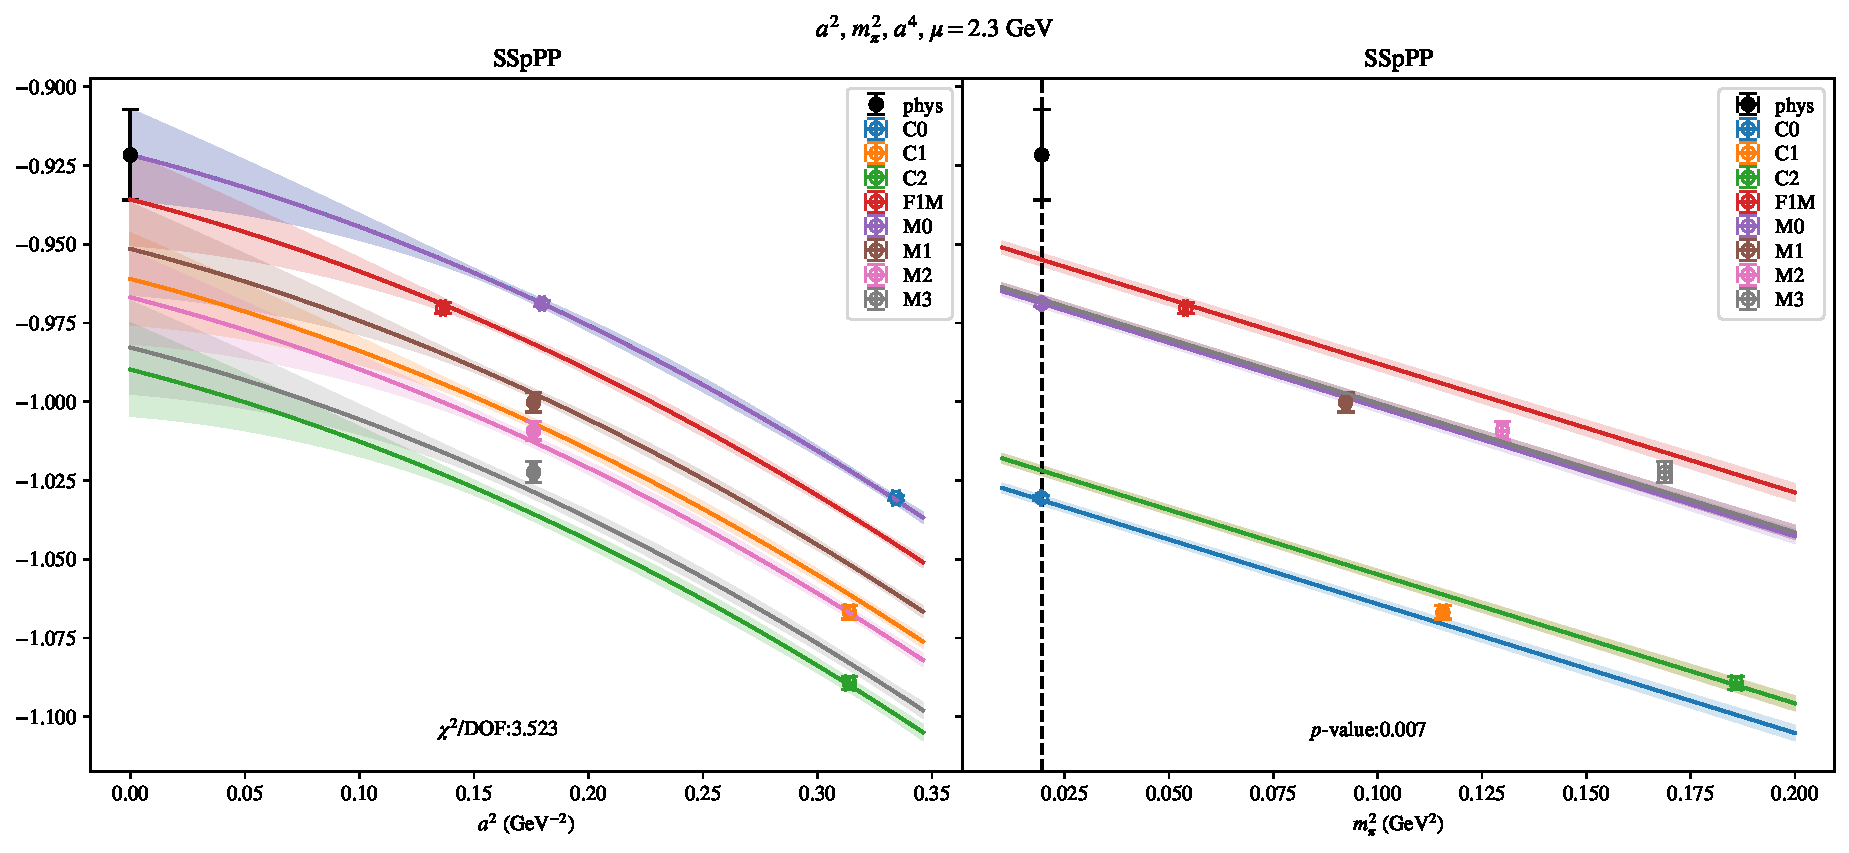
\includepdf[link, pages=-]{VVmAA/SUSY/bag_a2a4m2_23.pdf}
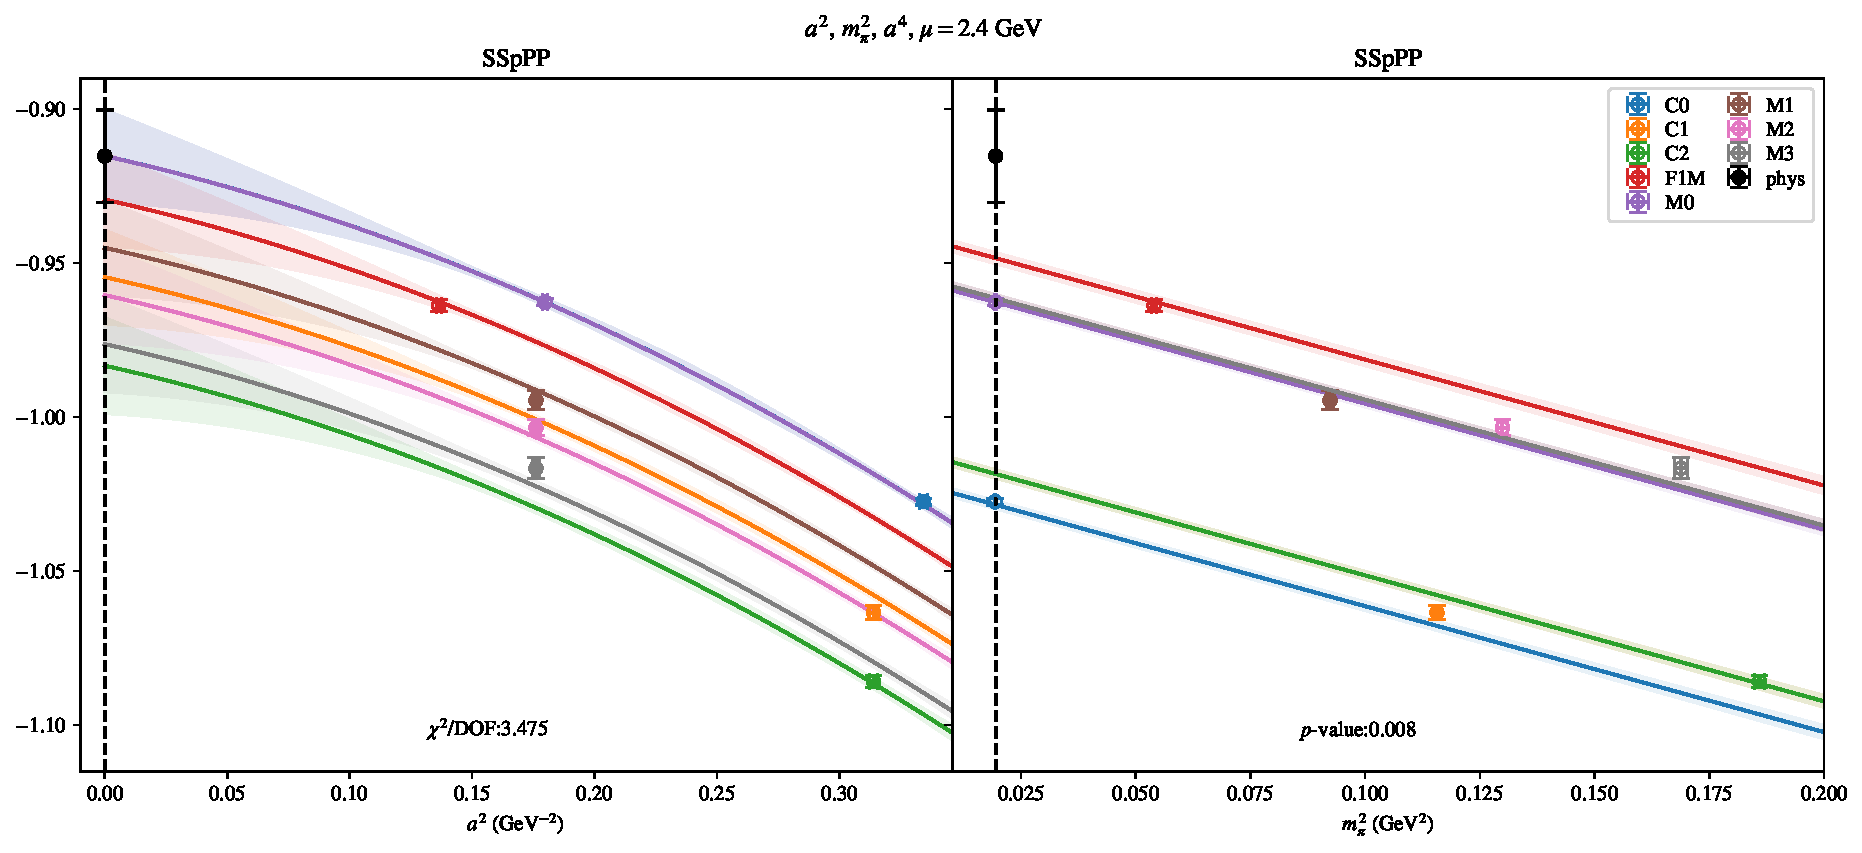
\includepdf[link, pages=-]{VVmAA/SUSY/bag_a2a4m2_24.pdf}
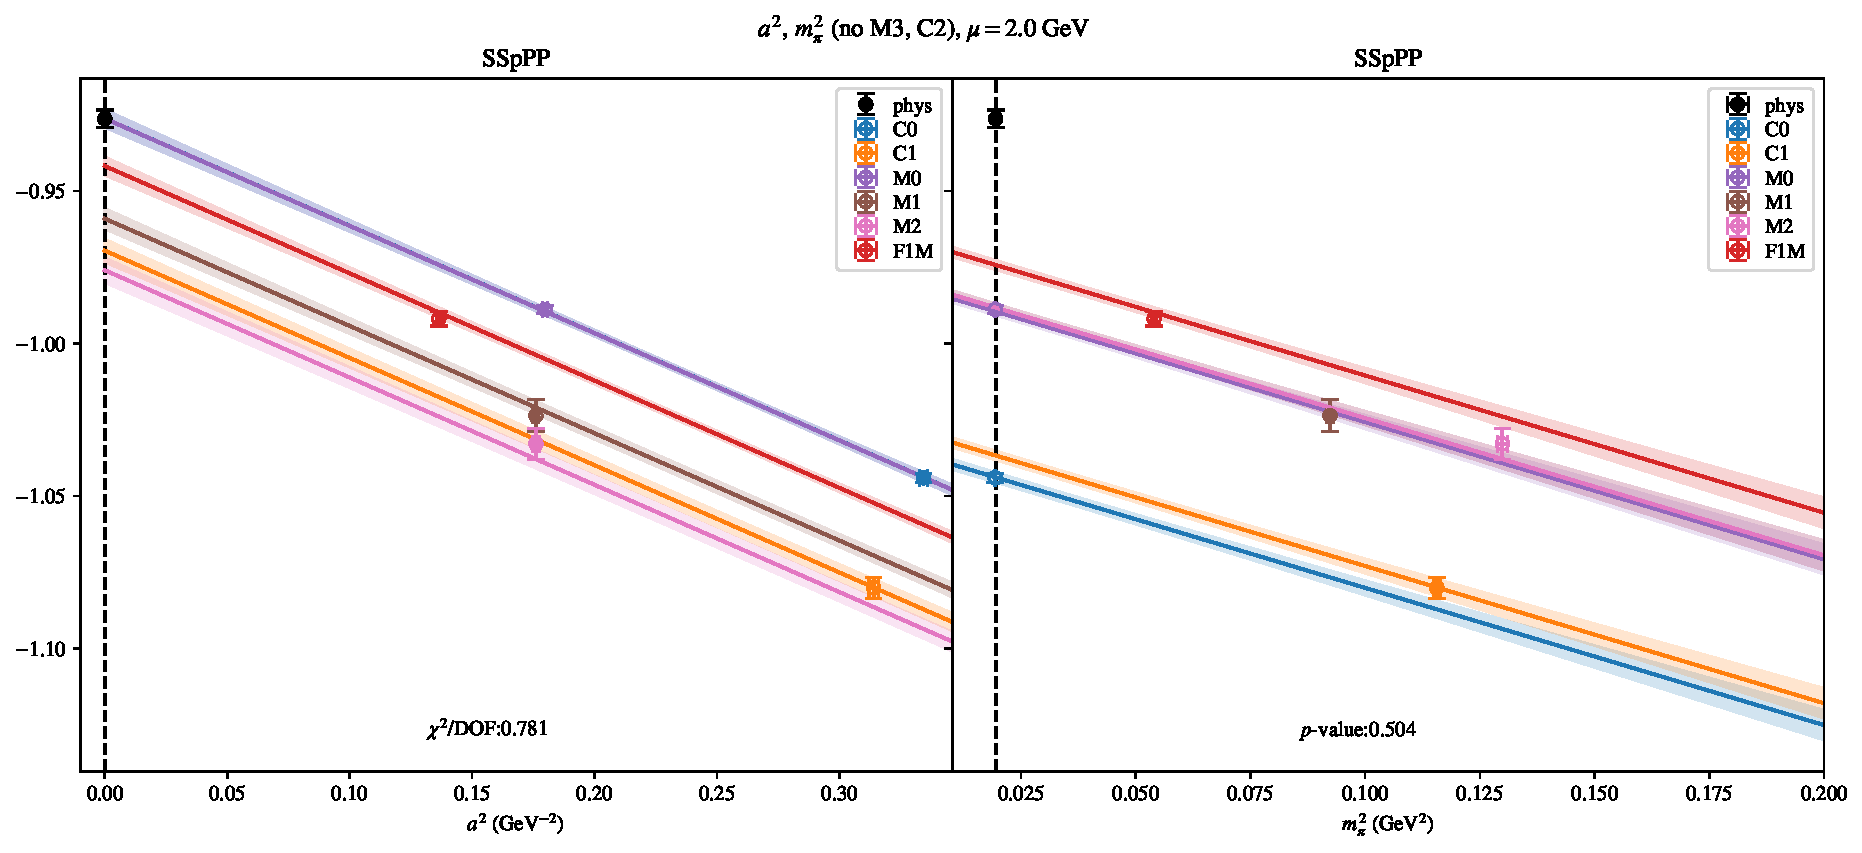
\includepdf[link, pages=-]{VVmAA/SUSY/bag_a2m2mcut_20.pdf}
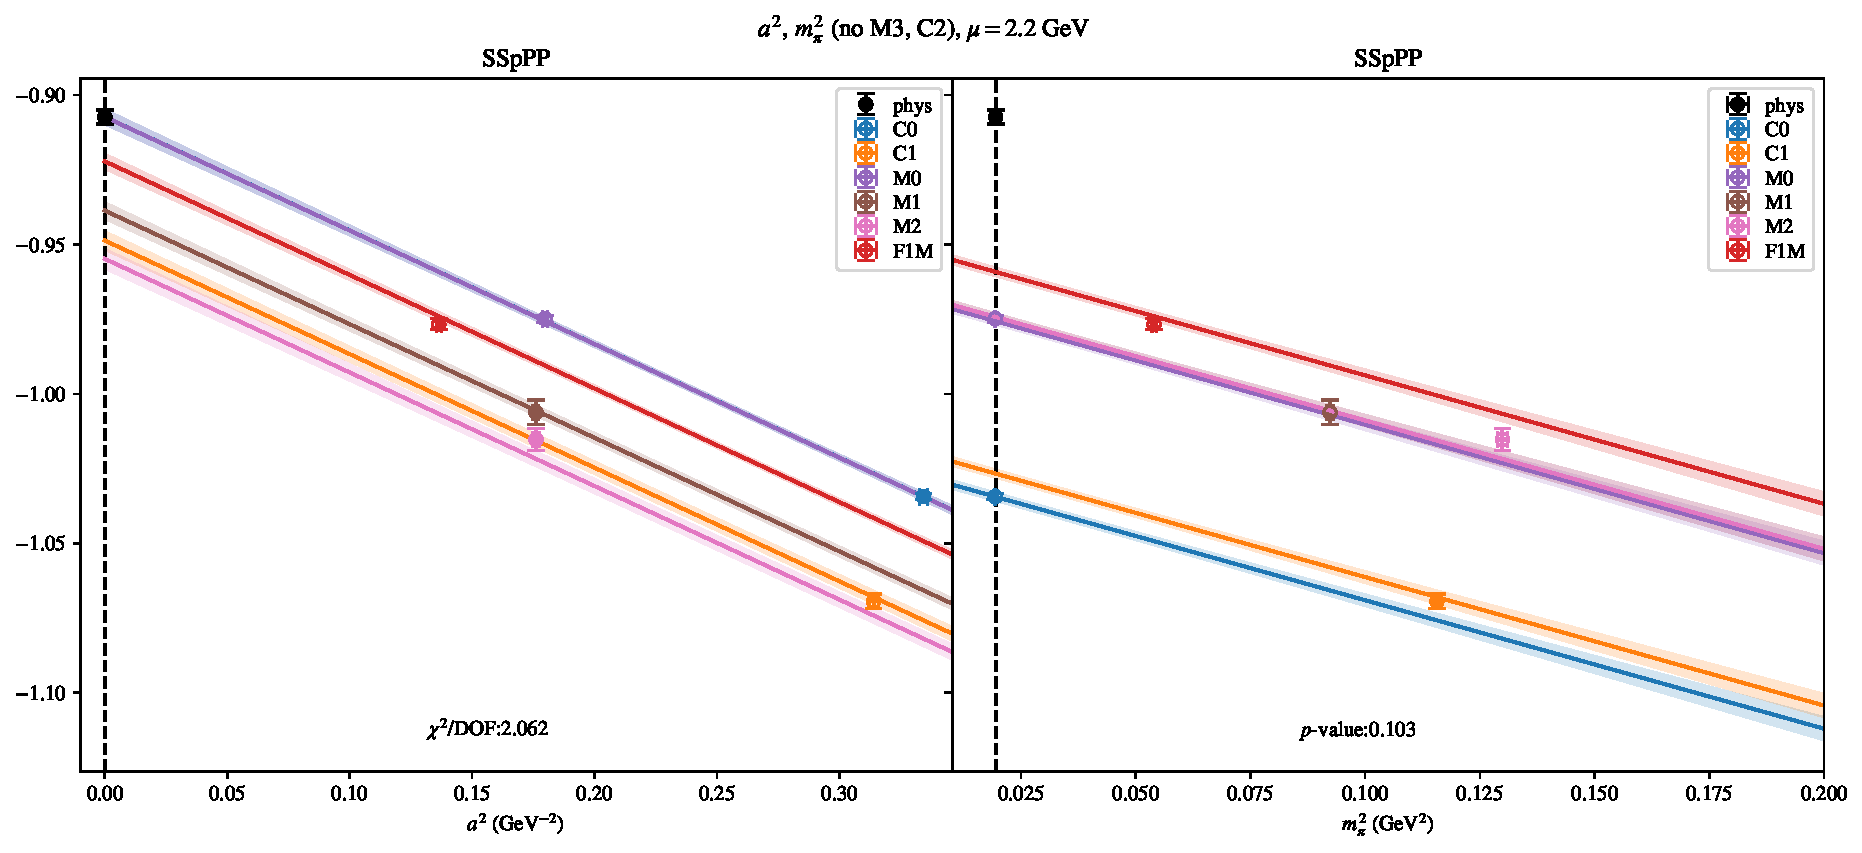
\includepdf[link, pages=-]{VVmAA/SUSY/bag_a2m2mcut_22.pdf}
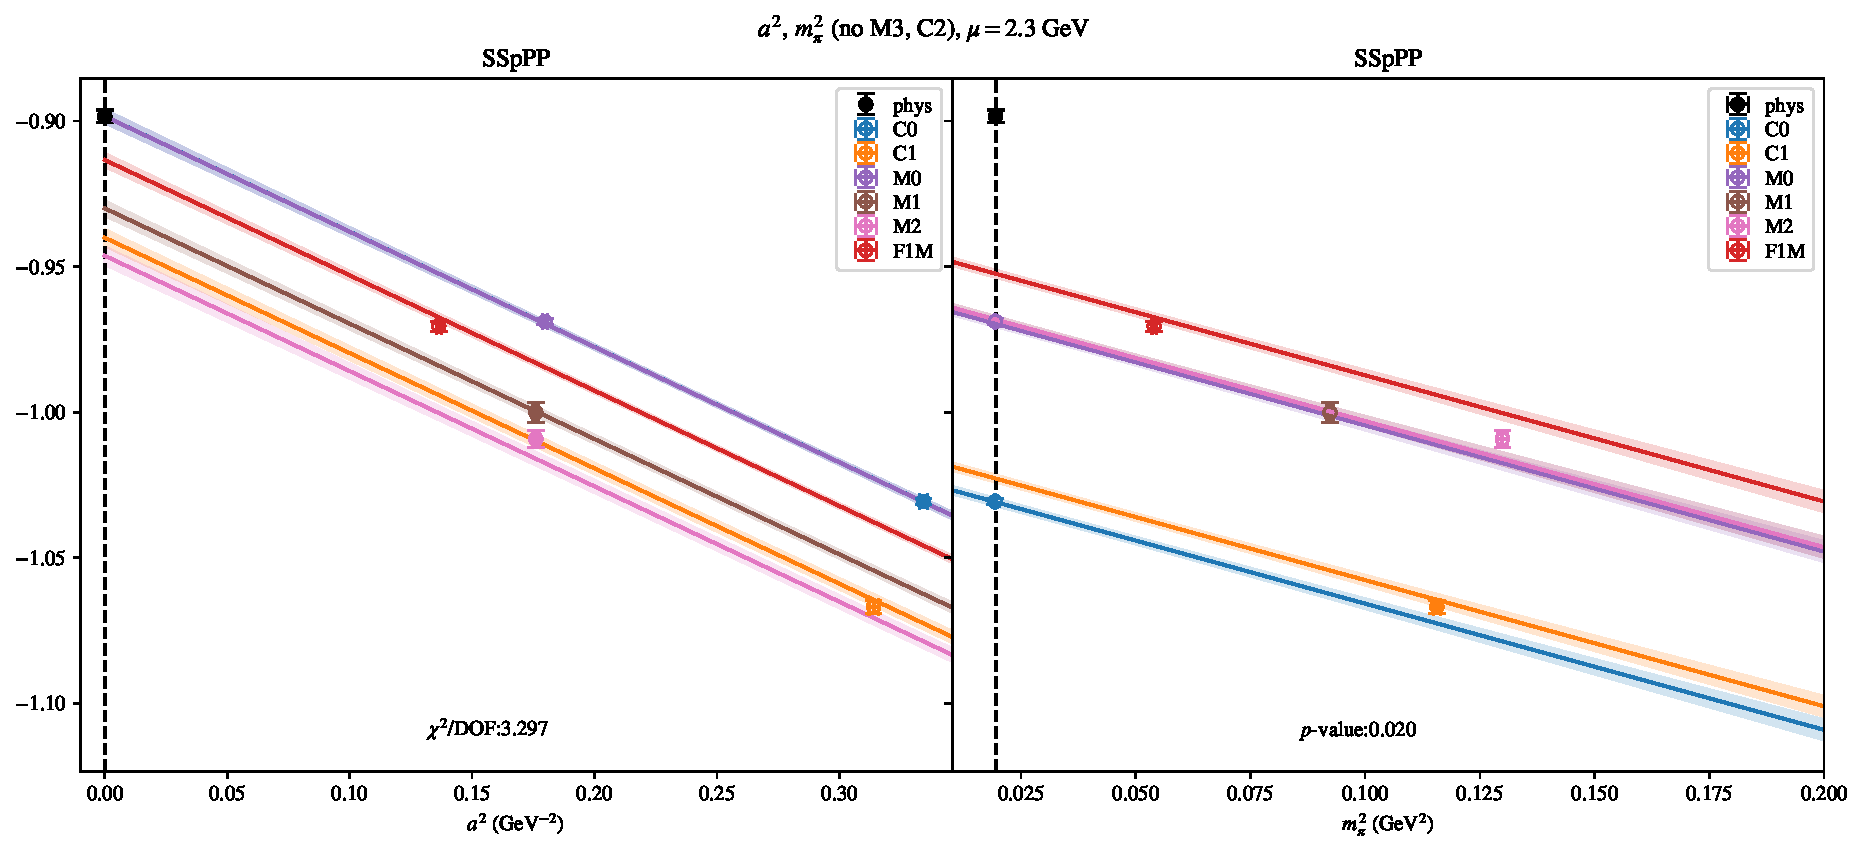
\includepdf[link, pages=-]{VVmAA/SUSY/bag_a2m2mcut_23.pdf}
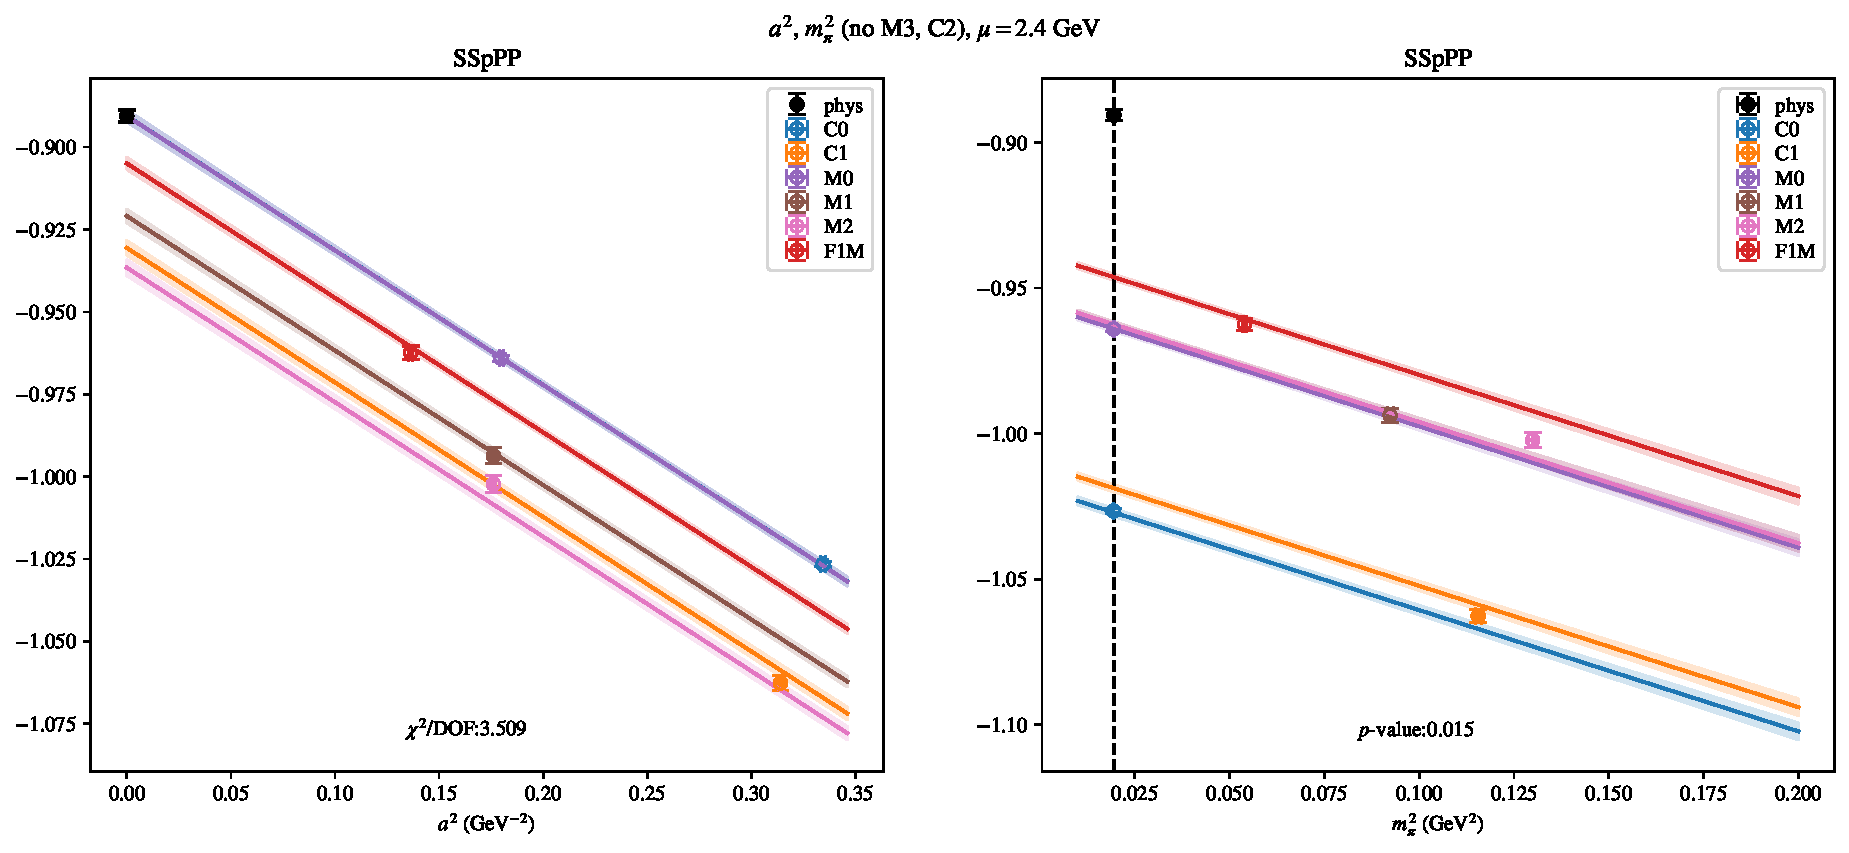
\includepdf[link, pages=-]{VVmAA/SUSY/bag_a2m2mcut_24.pdf}
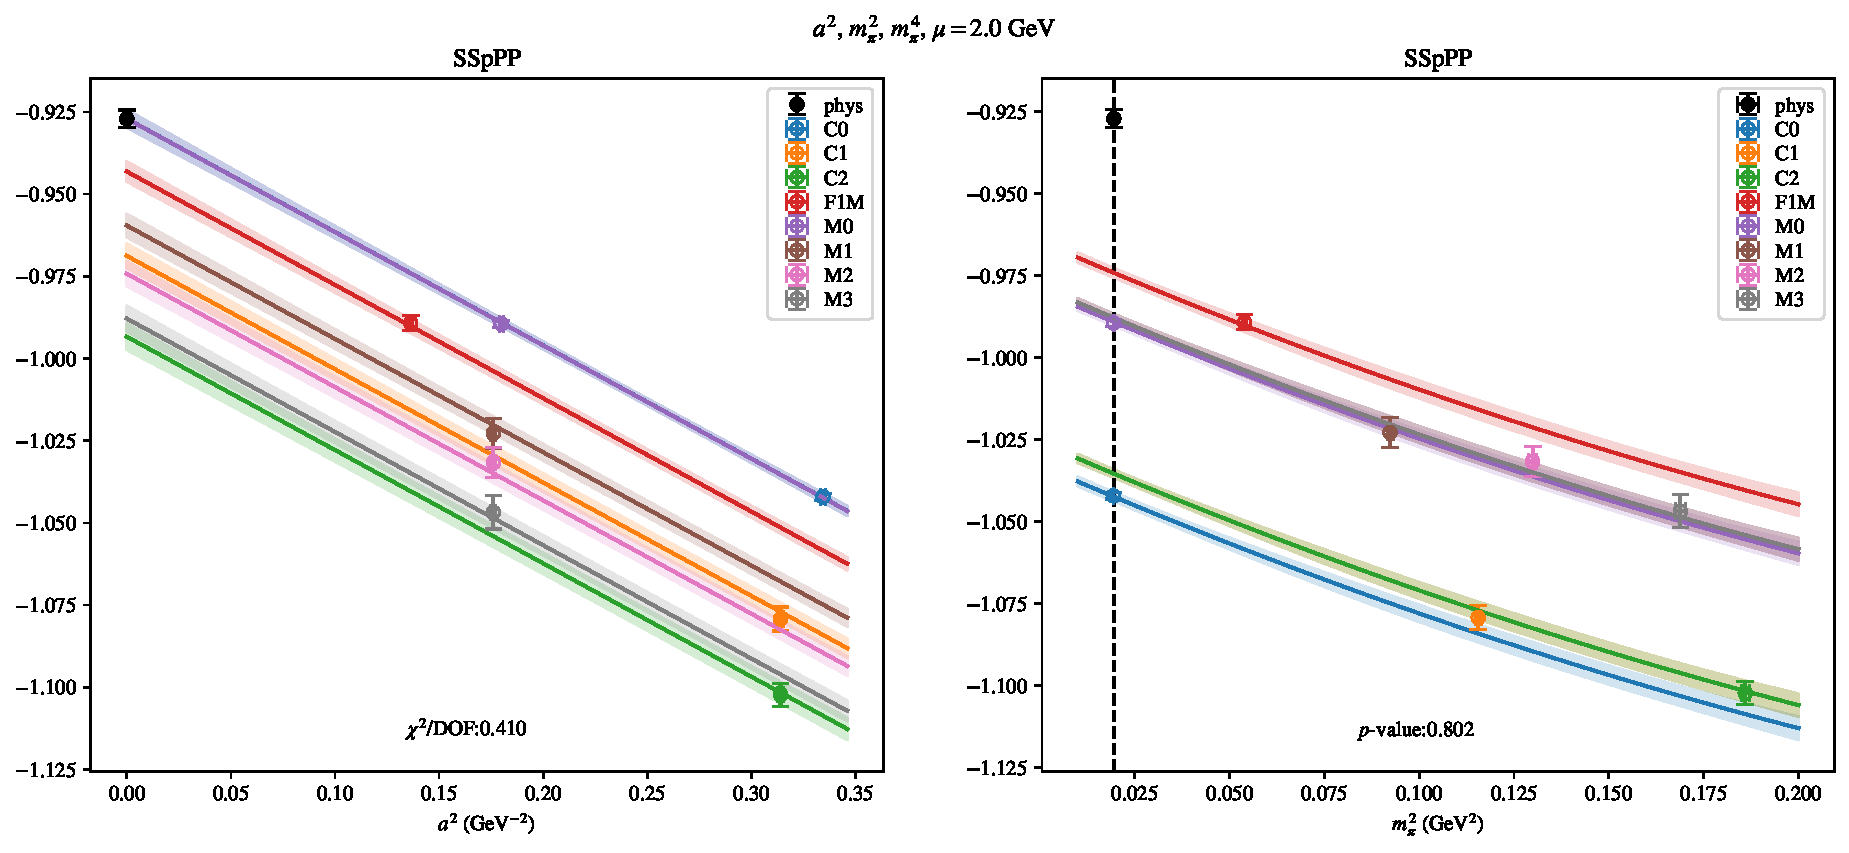
\includepdf[link, pages=-]{VVmAA/SUSY/bag_a2m2m4_20.pdf}
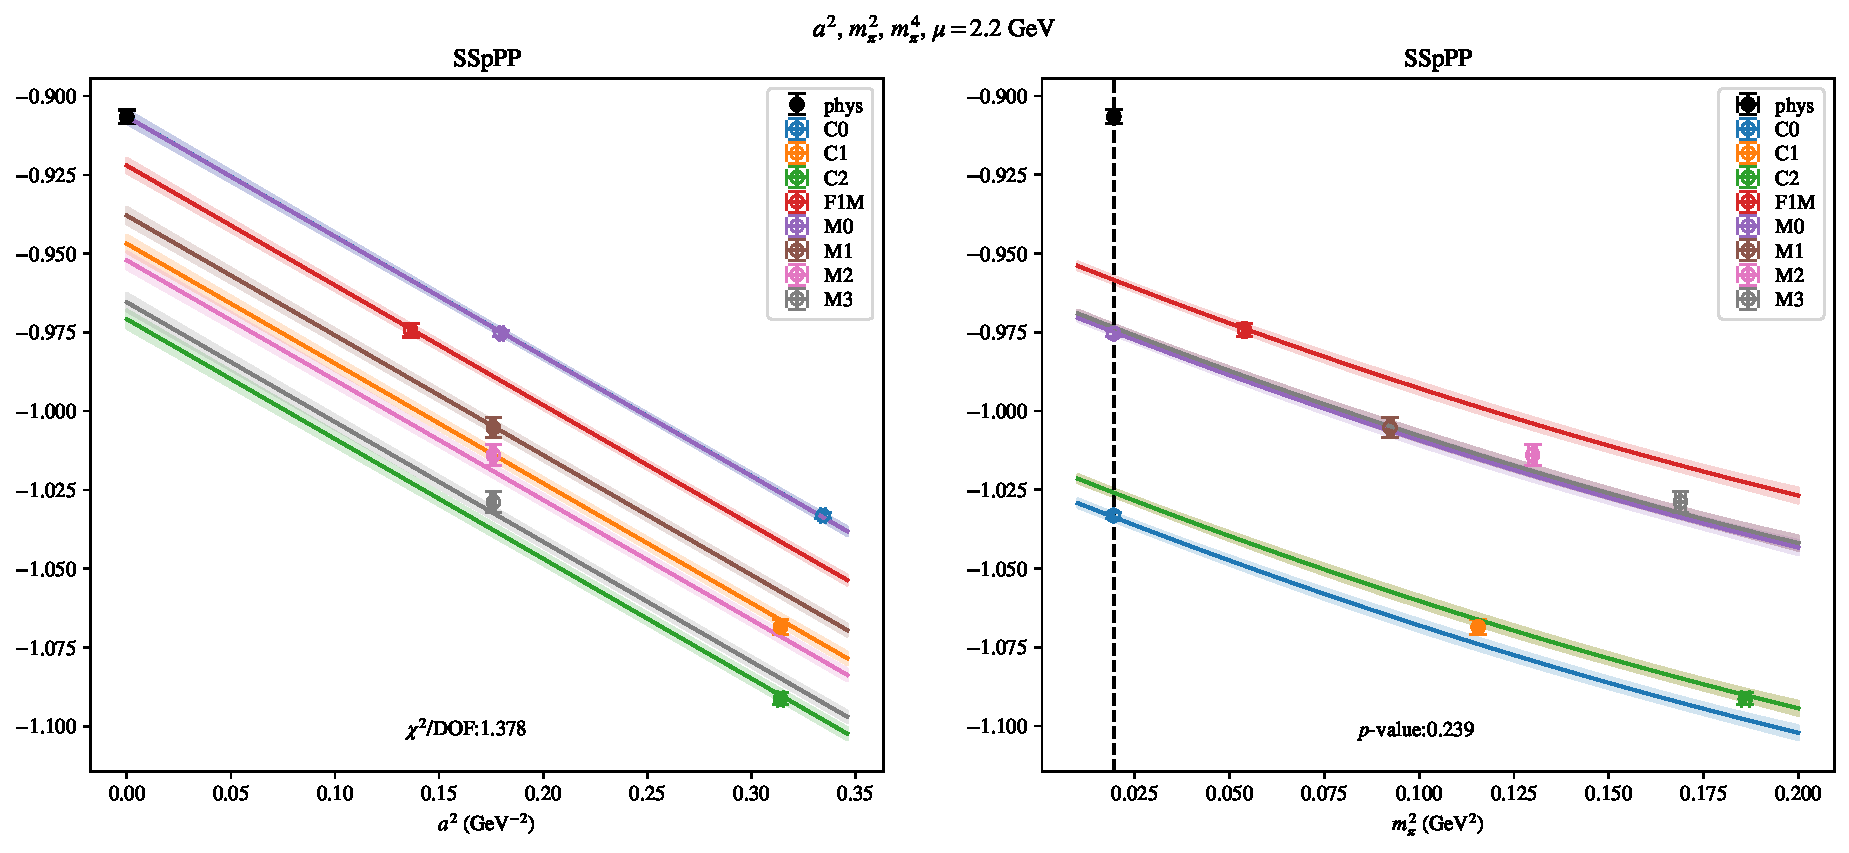
\includepdf[link, pages=-]{VVmAA/SUSY/bag_a2m2m4_22.pdf}
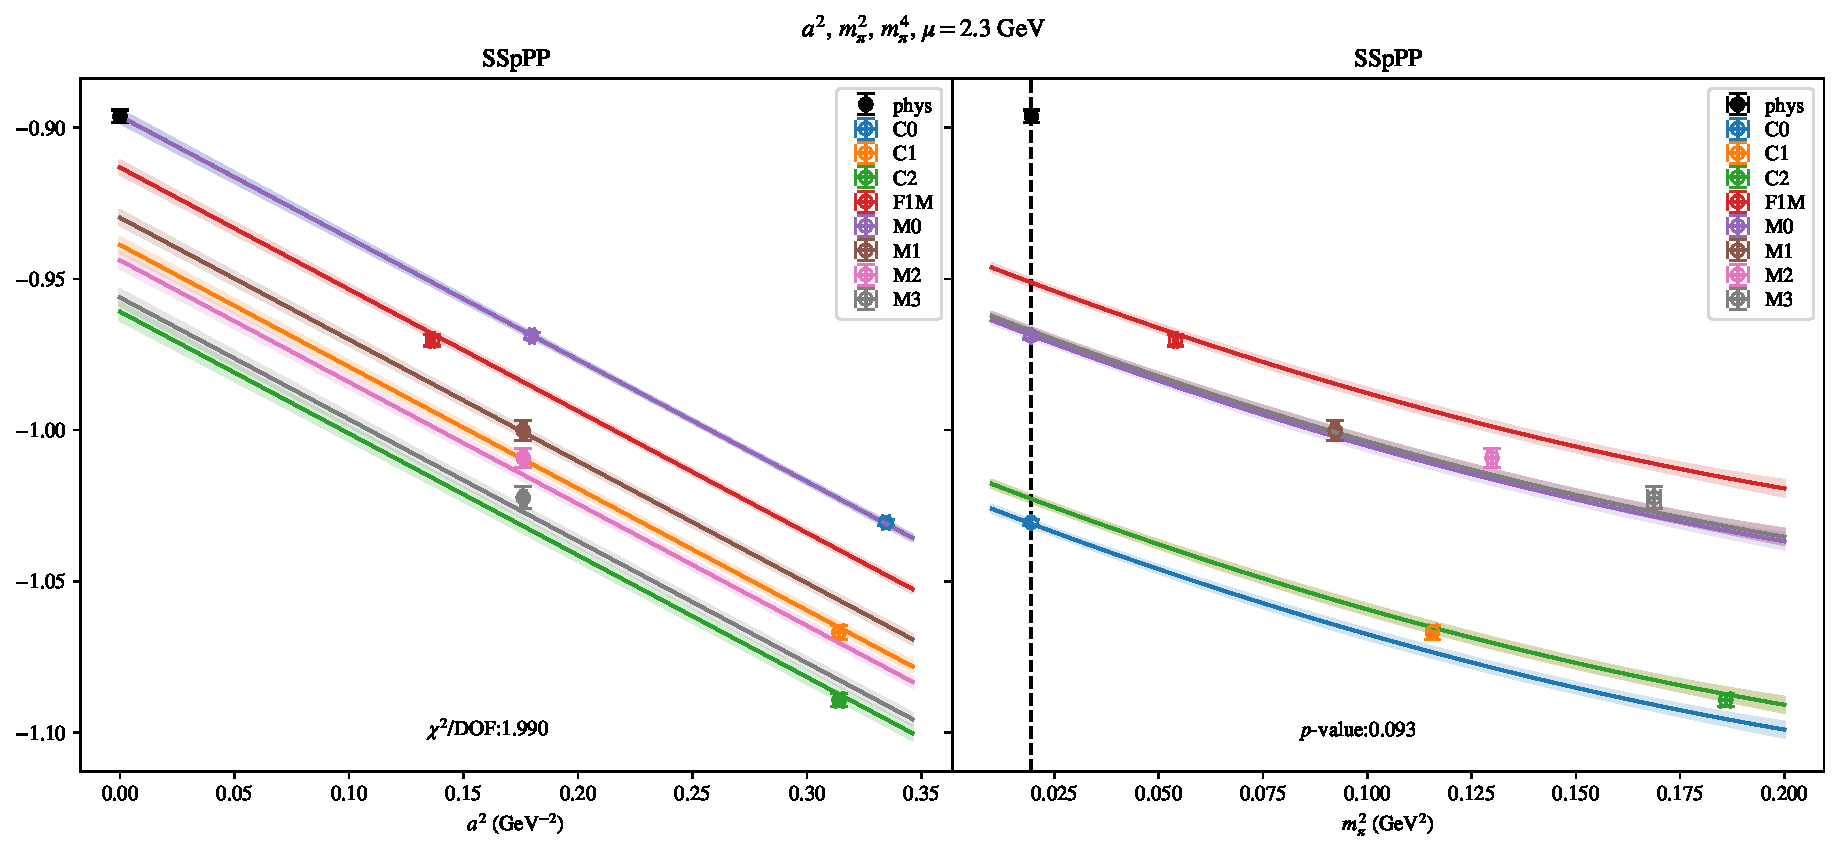
\includepdf[link, pages=-]{VVmAA/SUSY/bag_a2m2m4_23.pdf}
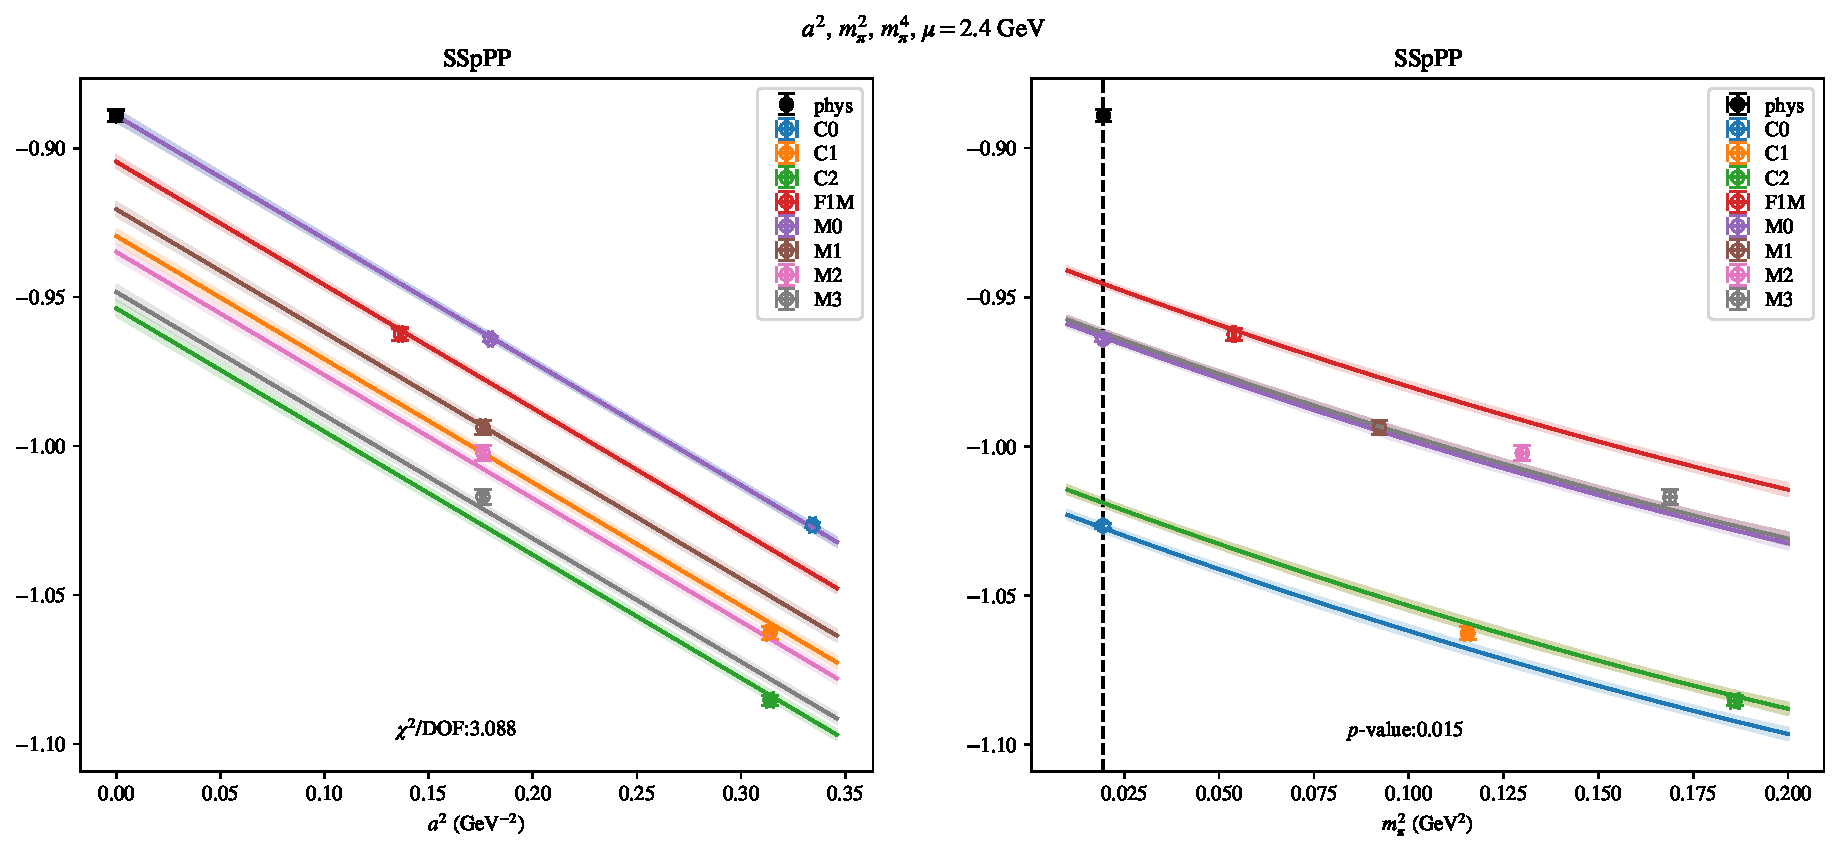
\includepdf[link, pages=-]{VVmAA/SUSY/bag_a2m2m4_24.pdf}
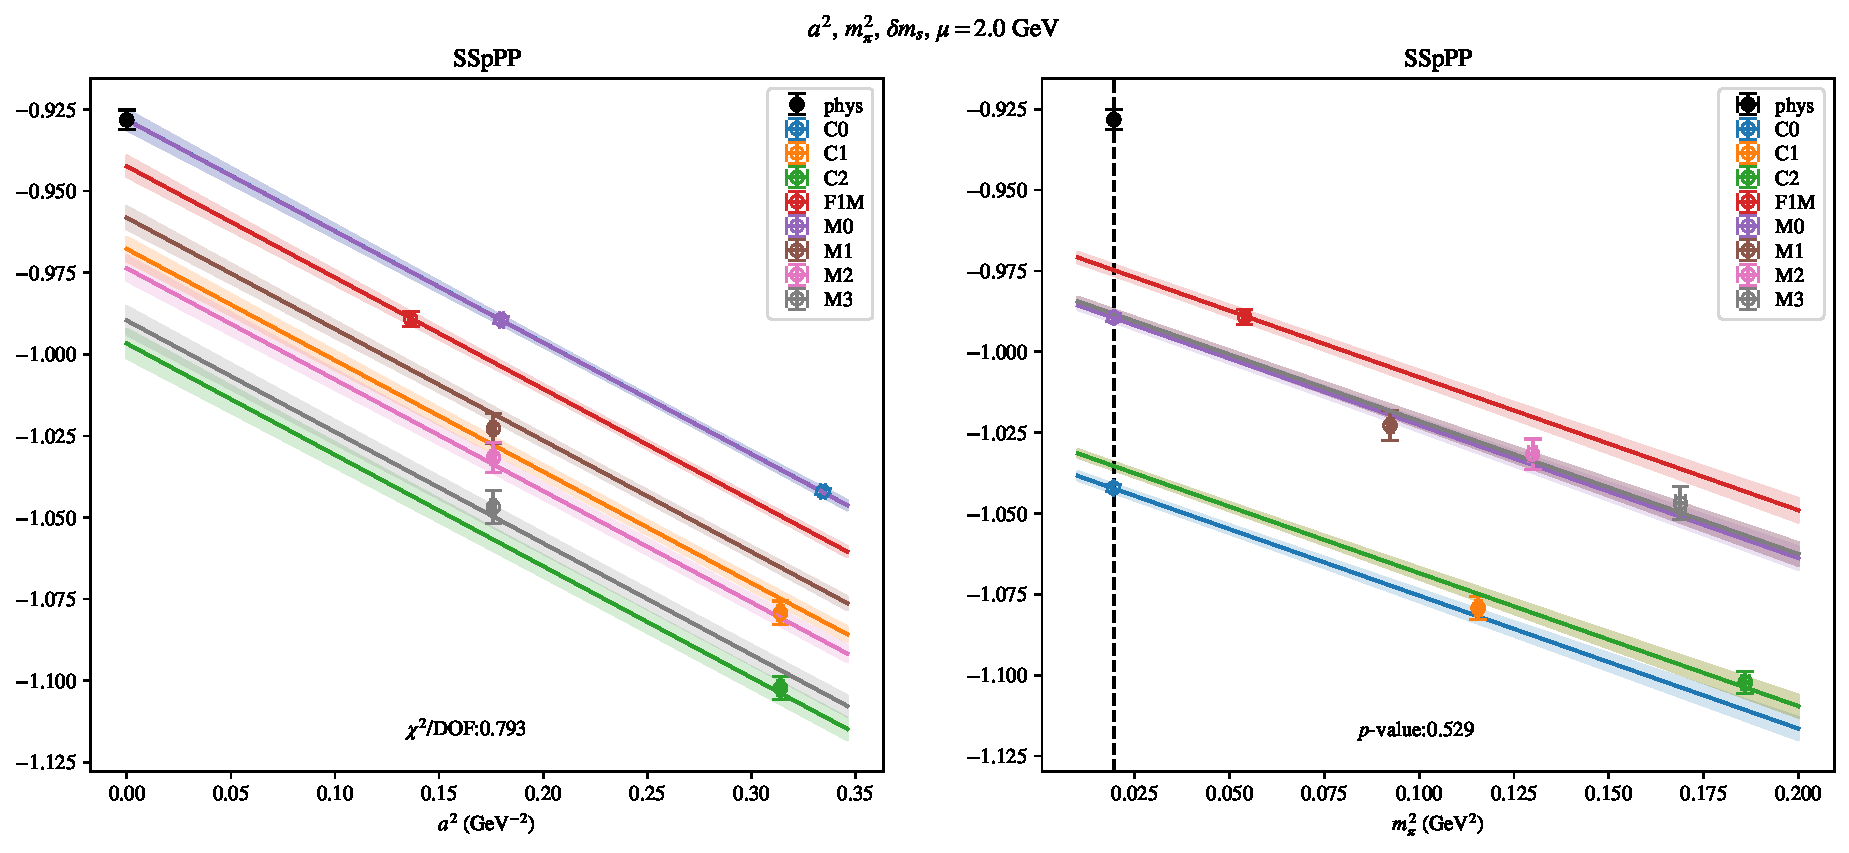
\includepdf[link, pages=-]{VVmAA/SUSY/bag_a2m2delm_20.pdf}
\includepdf[link, pages=-]{VVmAA/SUSY/bag_a2m2delm_22.pdf}
\includepdf[link, pages=-]{VVmAA/SUSY/bag_a2m2delm_23.pdf}
\includepdf[link, pages=-]{VVmAA/SUSY/bag_a2m2delm_24.pdf}
\clearpage
\section{$\mathcal{B}_3$}
\begin{table}[h!]
\begin{center}
\begin{tabular}{|c|c|c|c|c|c|c|}
\hline
$\mu$ (GeV) & $a^2$, $m_\pi^2$& $a^2$, $m_\pi^2$ (no C)& $a^2$, $m_\pi^2$, $a^4$& $a^2$, $m_\pi^2$ (no M3, C2)& $a^2$, $m_\pi^2$, $m_\pi^4$& $a^2$, $m_\pi^2$, $\delta m_s$\\
\hline
2.0& \hyperlink{SSmPP/SUSY/bag_a2m2_20.pdf.1}{\textbf{0.2815(22)}: 0.675 (0.642)} & \hyperlink{SSmPP/SUSY/bag_a2m2noC_20.pdf.1}{\textbf{0.2880(97)}: 0.581 (0.559)} & \hyperlink{SSmPP/SUSY/bag_a2a4m2_20.pdf.1}{\textbf{0.284(16)}: 0.84 (0.5)} & \hyperlink{SSmPP/SUSY/bag_a2m2mcut_20.pdf.1}{\textbf{0.2809(26)}: 0.604 (0.612)} & \hyperlink{SSmPP/SUSY/bag_a2m2m4_20.pdf.1}{\textbf{0.2800(27)}: 0.444 (0.777)} & \hyperlink{SSmPP/SUSY/bag_a2m2delm_20.pdf.1}{\textbf{0.2813(22)}: 0.746 (0.561)}\\
2.2& \hyperlink{SSmPP/SUSY/bag_a2m2_22.pdf.1}{\textbf{0.2725(20)}: 1.037 (0.394)} & \hyperlink{SSmPP/SUSY/bag_a2m2noC_22.pdf.1}{\textbf{0.2808(84)}: 0.531 (0.588)} & \hyperlink{SSmPP/SUSY/bag_a2a4m2_22.pdf.1}{\textbf{0.275(15)}: 1.317 (0.261)} & \hyperlink{SSmPP/SUSY/bag_a2m2mcut_22.pdf.1}{\textbf{0.2726(22)}: 0.86 (0.461)} & \hyperlink{SSmPP/SUSY/bag_a2m2m4_22.pdf.1}{\textbf{0.2714(21)}: 0.727 (0.573)} & \hyperlink{SSmPP/SUSY/bag_a2m2delm_22.pdf.1}{\textbf{0.2727(18)}: 1.174 (0.32)}\\
2.3& \hyperlink{SSmPP/SUSY/bag_a2m2_23.pdf.1}{\textbf{0.2691(16)}: 1.273 (0.272)} & \hyperlink{SSmPP/SUSY/bag_a2m2noC_23.pdf.1}{\textbf{0.2782(79)}: 0.578 (0.561)} & \hyperlink{SSmPP/SUSY/bag_a2a4m2_23.pdf.1}{\textbf{0.274(13)}: 1.57 (0.179)} & \hyperlink{SSmPP/SUSY/bag_a2m2mcut_23.pdf.1}{\textbf{0.2688(19)}: 1.188 (0.313)} & \hyperlink{SSmPP/SUSY/bag_a2m2m4_23.pdf.1}{\textbf{0.2675(18)}: 1.015 (0.398)} & \hyperlink{SSmPP/SUSY/bag_a2m2delm_23.pdf.1}{\textbf{0.2685(18)}: 1.446 (0.216)}\\
2.4& \hyperlink{SSmPP/SUSY/bag_a2m2_24.pdf.1}{\textbf{0.2651(16)}: 1.763 (0.117)} & \hyperlink{SSmPP/SUSY/bag_a2m2noC_24.pdf.1}{\textbf{0.2749(74)}: 0.681 (0.506)} & \hyperlink{SSmPP/SUSY/bag_a2a4m2_24.pdf.1}{\textbf{0.270(12)}: 2.169 (0.07)} & \hyperlink{SSmPP/SUSY/bag_a2m2mcut_24.pdf.1}{\textbf{0.2653(19)}: 1.523 (0.206)} & \hyperlink{SSmPP/SUSY/bag_a2m2m4_24.pdf.1}{\textbf{0.2639(18)}: 1.293 (0.27)} & \hyperlink{SSmPP/SUSY/bag_a2m2delm_24.pdf.1}{\textbf{0.2652(17)}: 1.892 (0.109)}\\
\hline
\end{tabular}
\caption{Physical point value from chiral and continuum extrapolation at renormalisation scale $\mu$. Entries are \textbf{value(error)}: $\chi^2/\text{DOF}$ ($p$-value).}
\end{center}
\end{table}
\begin{table}[h!]
\begin{center}
\begin{tabular}{|c c|c|c|c|c|c|c|}
\hline
$\mu$ (GeV) &  & $a^2$, $m_\pi^2$& $a^2$, $m_\pi^2$ (no C)& $a^2$, $m_\pi^2$, $a^4$& $a^2$, $m_\pi^2$ (no M3, C2)& $a^2$, $m_\pi^2$, $m_\pi^4$& $a^2$, $m_\pi^2$, $\delta m_s$\\
\hline
\multirow{3}{0.5in}{2.0} & $\alpha$ & 0.1828(80)& 0.147(56)& 0.16(15)& 0.1838(93)& 0.1865(94)& 0.1827(82)\\
 & $\beta$ & 0.00195(16)& 0.00180(31)& 0.00200(17)& 0.00223(25)& 0.00292(89)& 0.00176(38)\\
 & $\gamma$ &  &  & 0.04(30)&  & -0.000084(78)& 0.008(14)\\
\hline
\multirow{3}{0.5in}{2.2} & $\alpha$ & 0.2088(71)& 0.165(50)& 0.18(14)& 0.2077(75)& 0.2117(70)& 0.2076(67)\\
 & $\beta$ & 0.00208(14)& 0.00183(26)& 0.00210(16)& 0.00232(24)& 0.00305(73)& 0.00188(29)\\
 & $\gamma$ &  &  & 0.05(29)&  & -0.000085(63)& 0.008(10)\\
\hline
\multirow{3}{0.5in}{2.3} & $\alpha$ & 0.2195(57)& 0.169(46)& 0.18(12)& 0.2198(69)& 0.2242(61)& 0.2206(66)\\
 & $\beta$ & 0.00209(12)& 0.00185(23)& 0.00214(14)& 0.00232(22)& 0.00307(64)& 0.00187(31)\\
 & $\gamma$ &  &  & 0.09(25)&  & -0.000086(54)& 0.009(11)\\
\hline
\multirow{3}{0.5in}{2.4} & $\alpha$ & 0.2324(58)& 0.181(44)& 0.19(11)& 0.2310(65)& 0.2361(62)& 0.2316(61)\\
 & $\beta$ & 0.00215(10)& 0.00186(21)& 0.00215(13)& 0.00236(19)& 0.00305(55)& 0.00190(27)\\
 & $\gamma$ &  &  & 0.08(24)&  & -0.000083(48)& 0.009(10)\\
\hline
\end{tabular}
\caption{Fit values of coefficients in $Q = Q_{phys} + \mathbf{\alpha} a^2 + \mathbf{\beta}\left(\frac{m_\pi^2}{f_\pi^2}-\frac{m_{\pi,PDG}^2}{f_\pi^2}\right) + \gamma(\ldots)$}
\end{center}
\end{table}
\includepdf[link, pages=-]{SSmPP/SUSY/bag_a2m2_20.pdf}
\includepdf[link, pages=-]{SSmPP/SUSY/bag_a2m2_22.pdf}
\includepdf[link, pages=-]{SSmPP/SUSY/bag_a2m2_23.pdf}
\includepdf[link, pages=-]{SSmPP/SUSY/bag_a2m2_24.pdf}
\includepdf[link, pages=-]{SSmPP/SUSY/bag_a2m2noC_20.pdf}
\includepdf[link, pages=-]{SSmPP/SUSY/bag_a2m2noC_22.pdf}
\includepdf[link, pages=-]{SSmPP/SUSY/bag_a2m2noC_23.pdf}
\includepdf[link, pages=-]{SSmPP/SUSY/bag_a2m2noC_24.pdf}
\includepdf[link, pages=-]{SSmPP/SUSY/bag_a2a4m2_20.pdf}
\includepdf[link, pages=-]{SSmPP/SUSY/bag_a2a4m2_22.pdf}
\includepdf[link, pages=-]{SSmPP/SUSY/bag_a2a4m2_23.pdf}
\includepdf[link, pages=-]{SSmPP/SUSY/bag_a2a4m2_24.pdf}
\includepdf[link, pages=-]{SSmPP/SUSY/bag_a2m2mcut_20.pdf}
\includepdf[link, pages=-]{SSmPP/SUSY/bag_a2m2mcut_22.pdf}
\includepdf[link, pages=-]{SSmPP/SUSY/bag_a2m2mcut_23.pdf}
\includepdf[link, pages=-]{SSmPP/SUSY/bag_a2m2mcut_24.pdf}
\includepdf[link, pages=-]{SSmPP/SUSY/bag_a2m2m4_20.pdf}
\includepdf[link, pages=-]{SSmPP/SUSY/bag_a2m2m4_22.pdf}
\includepdf[link, pages=-]{SSmPP/SUSY/bag_a2m2m4_23.pdf}
\includepdf[link, pages=-]{SSmPP/SUSY/bag_a2m2m4_24.pdf}
\includepdf[link, pages=-]{SSmPP/SUSY/bag_a2m2delm_20.pdf}
\includepdf[link, pages=-]{SSmPP/SUSY/bag_a2m2delm_22.pdf}
\includepdf[link, pages=-]{SSmPP/SUSY/bag_a2m2delm_23.pdf}
\includepdf[link, pages=-]{SSmPP/SUSY/bag_a2m2delm_24.pdf}
\clearpage
\section{$\mathcal{B}_4$}
\begin{table}[h!]
\begin{center}
\begin{tabular}{|c|c|c|c|c|c|c|}
\hline
$\mu$ (GeV) & $a^2$, $m_\pi^2$& $a^2$, $m_\pi^2$ (no C)& $a^2$, $m_\pi^2$, $a^4$& $a^2$, $m_\pi^2$ (no M3, C2)& $a^2$, $m_\pi^2$, $m_\pi^4$& $a^2$, $m_\pi^2$, $\delta m_s$\\
\hline
2.0& \hyperlink{SSpPP/SUSY/bag_a2m2_20.pdf.1}{\textbf{1.7932(29)}: 9.949 (0.0)} & \hyperlink{SSpPP/SUSY/bag_a2m2noC_20.pdf.1}{\textbf{1.706(13)}: 0.217 (0.805)} & \hyperlink{SSpPP/SUSY/bag_a2a4m2_20.pdf.1}{\textbf{1.647(22)}: 0.809 (0.519)} & \hyperlink{SSpPP/SUSY/bag_a2m2mcut_20.pdf.1}{\textbf{1.7947(35)}: 16.218 (0.0)} & \hyperlink{SSpPP/SUSY/bag_a2m2m4_20.pdf.1}{\textbf{1.7981(35)}: 10.434 (0.0)} & \hyperlink{SSpPP/SUSY/bag_a2m2delm_20.pdf.1}{\textbf{1.7933(34)}: 5.338 (0.0)}\\
2.2& \hyperlink{SSpPP/SUSY/bag_a2m2_22.pdf.1}{\textbf{1.7996(28)}: 8.75 (0.0)} & \hyperlink{SSpPP/SUSY/bag_a2m2noC_22.pdf.1}{\textbf{1.720(13)}: 0.169 (0.844)} & \hyperlink{SSpPP/SUSY/bag_a2a4m2_22.pdf.1}{\textbf{1.665(21)}: 1.012 (0.399)} & \hyperlink{SSpPP/SUSY/bag_a2m2mcut_22.pdf.1}{\textbf{1.8015(33)}: 13.776 (0.0)} & \hyperlink{SSpPP/SUSY/bag_a2m2m4_22.pdf.1}{\textbf{1.8044(34)}: 8.568 (0.0)} & \hyperlink{SSpPP/SUSY/bag_a2m2delm_22.pdf.1}{\textbf{1.7991(31)}: 6.374 (0.0)}\\
2.3& \hyperlink{SSpPP/SUSY/bag_a2m2_23.pdf.1}{\textbf{1.8021(28)}: 8.347 (0.0)} & \hyperlink{SSpPP/SUSY/bag_a2m2noC_23.pdf.1}{\textbf{1.725(12)}: 0.191 (0.826)} & \hyperlink{SSpPP/SUSY/bag_a2a4m2_23.pdf.1}{\textbf{1.671(21)}: 0.814 (0.516)} & \hyperlink{SSpPP/SUSY/bag_a2m2mcut_23.pdf.1}{\textbf{1.8032(33)}: 13.319 (0.0)} & \hyperlink{SSpPP/SUSY/bag_a2m2m4_23.pdf.1}{\textbf{1.8062(33)}: 8.462 (0.0)} & \hyperlink{SSpPP/SUSY/bag_a2m2delm_23.pdf.1}{\textbf{1.8015(30)}: 5.713 (0.0)}\\
2.4& \hyperlink{SSpPP/SUSY/bag_a2m2_24.pdf.1}{\textbf{1.8038(28)}: 7.745 (0.0)} & \hyperlink{SSpPP/SUSY/bag_a2m2noC_24.pdf.1}{\textbf{1.730(12)}: 0.187 (0.83)} & \hyperlink{SSpPP/SUSY/bag_a2a4m2_24.pdf.1}{\textbf{1.678(21)}: 0.763 (0.549)} & \hyperlink{SSpPP/SUSY/bag_a2m2mcut_24.pdf.1}{\textbf{1.8047(33)}: 12.372 (0.0)} & \hyperlink{SSpPP/SUSY/bag_a2m2m4_24.pdf.1}{\textbf{1.8073(33)}: 7.995 (0.0)} & \hyperlink{SSpPP/SUSY/bag_a2m2delm_24.pdf.1}{\textbf{1.8033(29)}: 5.229 (0.0)}\\
\hline
\end{tabular}
\caption{Physical point value from chiral and continuum extrapolation at renormalisation scale $\mu$. Entries are \textbf{value(error)}: $\chi^2/\text{DOF}$ ($p$-value).}
\end{center}
\end{table}
\begin{table}[h!]
\begin{center}
\begin{tabular}{|c c|c|c|c|c|c|c|}
\hline
$\mu$ (GeV) &  & $a^2$, $m_\pi^2$& $a^2$, $m_\pi^2$ (no C)& $a^2$, $m_\pi^2$, $a^4$& $a^2$, $m_\pi^2$ (no M3, C2)& $a^2$, $m_\pi^2$, $m_\pi^4$& $a^2$, $m_\pi^2$, $\delta m_s$\\
\hline
\multirow{3}{0.5in}{2.0} & $\alpha$ & 0.144(11)& 0.668(78)& 1.49(20)& 0.140(13)& 0.129(12)& 0.137(11)\\
 & $\beta$ & -0.00152(24)& -0.00172(50)& -0.00216(29)& -0.00187(44)& -0.0050(12)& -0.00407(56)\\
 & $\gamma$ &  &  & -2.74(41)&  & 0.00032(11)& 0.102(19)\\
\hline
\multirow{3}{0.5in}{2.2} & $\alpha$ & 0.152(10)& 0.632(76)& 1.39(19)& 0.146(12)& 0.138(12)& 0.147(11)\\
 & $\beta$ & -0.00094(22)& -0.00134(45)& -0.00157(25)& -0.00153(41)& -0.0048(12)& -0.00301(53)\\
 & $\gamma$ &  &  & -2.52(40)&  & 0.00035(11)& 0.082(18)\\
\hline
\multirow{3}{0.5in}{2.3} & $\alpha$ & 0.153(10)& 0.617(74)& 1.35(19)& 0.151(12)& 0.142(12)& 0.149(10)\\
 & $\beta$ & -0.00084(21)& -0.00124(46)& -0.00146(24)& -0.00126(39)& -0.0041(12)& -0.00285(53)\\
 & $\gamma$ &  &  & -2.44(39)&  & 0.00029(10)& 0.080(18)\\
\hline
\multirow{3}{0.5in}{2.4} & $\alpha$ & 0.156(10)& 0.603(76)& 1.31(19)& 0.153(12)& 0.146(11)& 0.152(10)\\
 & $\beta$ & -0.00077(21)& -0.00113(45)& -0.00136(24)& -0.00111(38)& -0.0038(11)& -0.00269(52)\\
 & $\gamma$ &  &  & -2.35(38)&  & 0.00027(10)& 0.076(18)\\
\hline
\end{tabular}
\caption{Fit values of coefficients in $Q = Q_{phys} + \mathbf{\alpha} a^2 + \mathbf{\beta}\left(\frac{m_\pi^2}{f_\pi^2}-\frac{m_{\pi,PDG}^2}{f_\pi^2}\right) + \gamma(\ldots)$}
\end{center}
\end{table}
\includepdf[link, pages=-]{SSpPP/SUSY/bag_a2m2_20.pdf}
\includepdf[link, pages=-]{SSpPP/SUSY/bag_a2m2_22.pdf}
\includepdf[link, pages=-]{SSpPP/SUSY/bag_a2m2_23.pdf}
\includepdf[link, pages=-]{SSpPP/SUSY/bag_a2m2_24.pdf}
\includepdf[link, pages=-]{SSpPP/SUSY/bag_a2m2noC_20.pdf}
\includepdf[link, pages=-]{SSpPP/SUSY/bag_a2m2noC_22.pdf}
\includepdf[link, pages=-]{SSpPP/SUSY/bag_a2m2noC_23.pdf}
\includepdf[link, pages=-]{SSpPP/SUSY/bag_a2m2noC_24.pdf}
\includepdf[link, pages=-]{SSpPP/SUSY/bag_a2a4m2_20.pdf}
\includepdf[link, pages=-]{SSpPP/SUSY/bag_a2a4m2_22.pdf}
\includepdf[link, pages=-]{SSpPP/SUSY/bag_a2a4m2_23.pdf}
\includepdf[link, pages=-]{SSpPP/SUSY/bag_a2a4m2_24.pdf}
\includepdf[link, pages=-]{SSpPP/SUSY/bag_a2m2mcut_20.pdf}
\includepdf[link, pages=-]{SSpPP/SUSY/bag_a2m2mcut_22.pdf}
\includepdf[link, pages=-]{SSpPP/SUSY/bag_a2m2mcut_23.pdf}
\includepdf[link, pages=-]{SSpPP/SUSY/bag_a2m2mcut_24.pdf}
\includepdf[link, pages=-]{SSpPP/SUSY/bag_a2m2m4_20.pdf}
\includepdf[link, pages=-]{SSpPP/SUSY/bag_a2m2m4_22.pdf}
\includepdf[link, pages=-]{SSpPP/SUSY/bag_a2m2m4_23.pdf}
\includepdf[link, pages=-]{SSpPP/SUSY/bag_a2m2m4_24.pdf}
\includepdf[link, pages=-]{SSpPP/SUSY/bag_a2m2delm_20.pdf}
\includepdf[link, pages=-]{SSpPP/SUSY/bag_a2m2delm_22.pdf}
\includepdf[link, pages=-]{SSpPP/SUSY/bag_a2m2delm_23.pdf}
\includepdf[link, pages=-]{SSpPP/SUSY/bag_a2m2delm_24.pdf}
\clearpage
\section{$\mathcal{B}_5$}
\begin{table}[h!]
\begin{center}
\begin{tabular}{|c|c|c|c|c|c|c|}
\hline
$\mu$ (GeV) & $a^2$, $m_\pi^2$& $a^2$, $m_\pi^2$ (no C)& $a^2$, $m_\pi^2$, $a^4$& $a^2$, $m_\pi^2$ (no M3, C2)& $a^2$, $m_\pi^2$, $m_\pi^4$& $a^2$, $m_\pi^2$, $\delta m_s$\\
\hline
2.0& \hyperlink{TT/SUSY/bag_a2m2_20.pdf.1}{\textbf{0.4930(38)}: 0.358 (0.878)} & \hyperlink{TT/SUSY/bag_a2m2noC_20.pdf.1}{\textbf{0.471(16)}: 0.093 (0.911)} & \hyperlink{TT/SUSY/bag_a2a4m2_20.pdf.1}{\textbf{0.458(32)}: 0.128 (0.972)} & \hyperlink{TT/SUSY/bag_a2m2mcut_20.pdf.1}{\textbf{0.4936(48)}: 0.599 (0.616)} & \hyperlink{TT/SUSY/bag_a2m2m4_20.pdf.1}{\textbf{0.4943(42)}: 0.498 (0.737)} & \hyperlink{TT/SUSY/bag_a2m2delm_20.pdf.1}{\textbf{0.4930(42)}: 0.336 (0.854)}\\
2.2& \hyperlink{TT/SUSY/bag_a2m2_22.pdf.1}{\textbf{0.5000(35)}: 0.394 (0.853)} & \hyperlink{TT/SUSY/bag_a2m2noC_22.pdf.1}{\textbf{0.480(15)}: 0.05 (0.951)} & \hyperlink{TT/SUSY/bag_a2a4m2_22.pdf.1}{\textbf{0.471(27)}: 0.16 (0.959)} & \hyperlink{TT/SUSY/bag_a2m2mcut_22.pdf.1}{\textbf{0.5005(40)}: 0.578 (0.629)} & \hyperlink{TT/SUSY/bag_a2m2m4_22.pdf.1}{\textbf{0.5011(39)}: 0.334 (0.855)} & \hyperlink{TT/SUSY/bag_a2m2delm_22.pdf.1}{\textbf{0.5001(37)}: 0.388 (0.817)}\\
2.3& \hyperlink{TT/SUSY/bag_a2m2_23.pdf.1}{\textbf{0.5031(32)}: 0.37 (0.87)} & \hyperlink{TT/SUSY/bag_a2m2noC_23.pdf.1}{\textbf{0.484(13)}: 0.045 (0.956)} & \hyperlink{TT/SUSY/bag_a2a4m2_23.pdf.1}{\textbf{0.473(26)}: 0.118 (0.976)} & \hyperlink{TT/SUSY/bag_a2m2mcut_23.pdf.1}{\textbf{0.5039(36)}: 0.646 (0.585)} & \hyperlink{TT/SUSY/bag_a2m2m4_23.pdf.1}{\textbf{0.5042(36)}: 0.413 (0.8)} & \hyperlink{TT/SUSY/bag_a2m2delm_23.pdf.1}{\textbf{0.5035(32)}: 0.388 (0.818)}\\
2.4& \hyperlink{TT/SUSY/bag_a2m2_24.pdf.1}{\textbf{0.5061(29)}: 0.39 (0.856)} & \hyperlink{TT/SUSY/bag_a2m2noC_24.pdf.1}{\textbf{0.487(12)}: 0.046 (0.955)} & \hyperlink{TT/SUSY/bag_a2a4m2_24.pdf.1}{\textbf{0.479(24)}: 0.158 (0.959)} & \hyperlink{TT/SUSY/bag_a2m2mcut_24.pdf.1}{\textbf{0.5062(34)}: 0.61 (0.608)} & \hyperlink{TT/SUSY/bag_a2m2m4_24.pdf.1}{\textbf{0.5070(33)}: 0.427 (0.789)} & \hyperlink{TT/SUSY/bag_a2m2delm_24.pdf.1}{\textbf{0.5060(30)}: 0.406 (0.805)}\\
\hline
\end{tabular}
\caption{Physical point value from chiral and continuum extrapolation at renormalisation scale $\mu$. Entries are \textbf{value(error)}: $\chi^2/\text{DOF}$ ($p$-value).}
\end{center}
\end{table}
\begin{table}[h!]
\begin{center}
\begin{tabular}{|c c|c|c|c|c|c|c|}
\hline
$\mu$ (GeV) &  & $a^2$, $m_\pi^2$& $a^2$, $m_\pi^2$ (no C)& $a^2$, $m_\pi^2$, $a^4$& $a^2$, $m_\pi^2$ (no M3, C2)& $a^2$, $m_\pi^2$, $m_\pi^4$& $a^2$, $m_\pi^2$, $\delta m_s$\\
\hline
\multirow{3}{0.5in}{2.0} & $\alpha$ & -0.083(13)& 0.05(10)& 0.24(29)& -0.085(16)& -0.087(14)& -0.084(14)\\
 & $\beta$ & 0.00074(23)& 0.00066(56)& 0.00054(32)& 0.00070(44)& 0.0002(13)& 0.00042(59)\\
 & $\gamma$ &  &  & -0.67(60)&  & 0.00005(11)& 0.013(21)\\
\hline
\multirow{3}{0.5in}{2.2} & $\alpha$ & -0.105(12)& 0.014(93)& 0.16(25)& -0.107(13)& -0.108(13)& -0.106(13)\\
 & $\beta$ & 0.00079(24)& 0.00069(40)& 0.00063(27)& 0.00067(40)& 0.0002(11)& 0.00059(54)\\
 & $\gamma$ &  &  & -0.54(51)&  & 0.000057(96)& 0.008(19)\\
\hline
\multirow{3}{0.5in}{2.3} & $\alpha$ & -0.117(11)& -0.001(83)& 0.16(24)& -0.119(12)& -0.120(12)& -0.119(11)\\
 & $\beta$ & 0.00080(20)& 0.00068(48)& 0.00062(28)& 0.00069(32)& 0.0003(10)& 0.00055(48)\\
 & $\gamma$ &  &  & -0.57(48)&  & 0.000047(87)& 0.009(17)\\
\hline
\multirow{3}{0.5in}{2.4} & $\alpha$ & -0.1298(99)& -0.017(76)& 0.12(22)& -0.130(11)& -0.132(10)& -0.130(10)\\
 & $\beta$ & 0.00077(18)& 0.00070(41)& 0.00061(23)& 0.00069(34)& 0.00029(93)& 0.00054(46)\\
 & $\gamma$ &  &  & -0.52(45)&  & 0.000041(81)& 0.009(16)\\
\hline
\end{tabular}
\caption{Fit values of coefficients in $Q = Q_{phys} + \mathbf{\alpha} a^2 + \mathbf{\beta}\left(\frac{m_\pi^2}{f_\pi^2}-\frac{m_{\pi,PDG}^2}{f_\pi^2}\right) + \gamma(\ldots)$}
\end{center}
\end{table}
\includepdf[link, pages=-]{TT/SUSY/bag_a2m2_20.pdf}
\includepdf[link, pages=-]{TT/SUSY/bag_a2m2_22.pdf}
\includepdf[link, pages=-]{TT/SUSY/bag_a2m2_23.pdf}
\includepdf[link, pages=-]{TT/SUSY/bag_a2m2_24.pdf}
\includepdf[link, pages=-]{TT/SUSY/bag_a2m2noC_20.pdf}
\includepdf[link, pages=-]{TT/SUSY/bag_a2m2noC_22.pdf}
\includepdf[link, pages=-]{TT/SUSY/bag_a2m2noC_23.pdf}
\includepdf[link, pages=-]{TT/SUSY/bag_a2m2noC_24.pdf}
\includepdf[link, pages=-]{TT/SUSY/bag_a2a4m2_20.pdf}
\includepdf[link, pages=-]{TT/SUSY/bag_a2a4m2_22.pdf}
\includepdf[link, pages=-]{TT/SUSY/bag_a2a4m2_23.pdf}
\includepdf[link, pages=-]{TT/SUSY/bag_a2a4m2_24.pdf}
\includepdf[link, pages=-]{TT/SUSY/bag_a2m2mcut_20.pdf}
\includepdf[link, pages=-]{TT/SUSY/bag_a2m2mcut_22.pdf}
\includepdf[link, pages=-]{TT/SUSY/bag_a2m2mcut_23.pdf}
\includepdf[link, pages=-]{TT/SUSY/bag_a2m2mcut_24.pdf}
\includepdf[link, pages=-]{TT/SUSY/bag_a2m2m4_20.pdf}
\includepdf[link, pages=-]{TT/SUSY/bag_a2m2m4_22.pdf}
\includepdf[link, pages=-]{TT/SUSY/bag_a2m2m4_23.pdf}
\includepdf[link, pages=-]{TT/SUSY/bag_a2m2m4_24.pdf}
\includepdf[link, pages=-]{TT/SUSY/bag_a2m2delm_20.pdf}
\includepdf[link, pages=-]{TT/SUSY/bag_a2m2delm_22.pdf}
\includepdf[link, pages=-]{TT/SUSY/bag_a2m2delm_23.pdf}
\includepdf[link, pages=-]{TT/SUSY/bag_a2m2delm_24.pdf}
\clearpage
\end{document}